% A pure minimalistic LaTeX-Beamer theme for everyone to use.
% Copyright (C) 2020 Kai Norman Clasen
% Edited by Lucas Saldyt

\documentclass[aspectratio=169]{beamer}
\DeclareMathSizes{12}{30}{16}{12}
% should also look nice for the classic aspectratio
% of course, than the text has to be refitted
% \documentclass{beamer} 
\usepackage[utf8]{inputenc}
\usepackage[T1]{fontenc}
\usepackage{tikz}
\usepackage{amsmath}
\usepackage[export]{adjustbox}
\usepackage[percent]{overpic}
\usepackage{epigraph}

\DeclareMathOperator*{\argmin}{\arg\!\min}
\DeclareMathOperator*{\argmax}{\arg\!\max}

\usetheme[showmaxslides, darkmode]{pureminimalistic}

\usepackage[american]{babel}
\usepackage{csquotes}
\usepackage[style=apa, backend=biber]{biblatex}
\DeclareLanguageMapping{american}{american-UoN}

% \usepackage[english]{babel}
% \usepackage[backend=biber,style=apa]{biblatex}
% \DeclareLanguageMapping{english}{english-apa}
\addbibresource{sources.bib}

% this makes it possible to add backup slides, without counting them
\usepackage{appendixnumberbeamer}
\renewcommand{\appendixname}{\texorpdfstring{\translate{appendix}}{appendix}}

\renewcommand{\logotitle}{
\includegraphics[width=.2\linewidth]{logos/asu_logo_alt.png}}
\renewcommand{\logoheader}{}
\renewcommand{\logofooter}{
\includegraphics[width=.15\linewidth]{logos/asu_logo_alt.png}}
\renewcommand{\emph}[1]{{\Huge \color{pureminimalistic@text@red} #1}}
\newcommand{\white}[1]{{\color{pureminimalistic@text@white} #1}}
\newcommand{\red}[1]{{\color{pureminimalistic@text@red} #1}}

\definecolor{c1}{RGB}{30, 76, 214}
\definecolor{c2}{RGB}{161, 3, 74}
\definecolor{c3}{RGB}{255, 132, 0}
\definecolor{c4}{RGB}{255, 196, 0}
\definecolor{c5}{RGB}{3, 171, 34}
\definecolor{grey}{RGB}{130, 130, 130}

\newcommand{m1}[1]{\color{c1}#1}
\newcommand{m2}[1]{\color{c1}#1}
\newcommand{m3}[1]{\color{c1}#1}
\newcommand{m4}[1]{\color{c1}#1}
\newcommand{m5}[1]{\color{c1}#1}

\title[Lifelong Learning for Planning]{Lifelong Learning for Robot Path-Planning}
\author{Lucas Saldyt}
\institute{Arizona State University} 
\date{\today}

\begin{document}

% Hello, I'm Lucas, and today I'll be presenting  "Lifelong Learning for Robot Path Planning"
\maketitle

\begin{frame}[plain]
  % This thesis focuses on environmental adaptation in robots.
  % An example robot is NASA's Perseverance rover, which was custom-engineered for mars.
  % Because of resource constraints and a desire for reliability, this rover doesn't use machine learning directly
  \begin{figure}
  \centering
  \vspace*{-1em}
  \hspace*{-3em}
  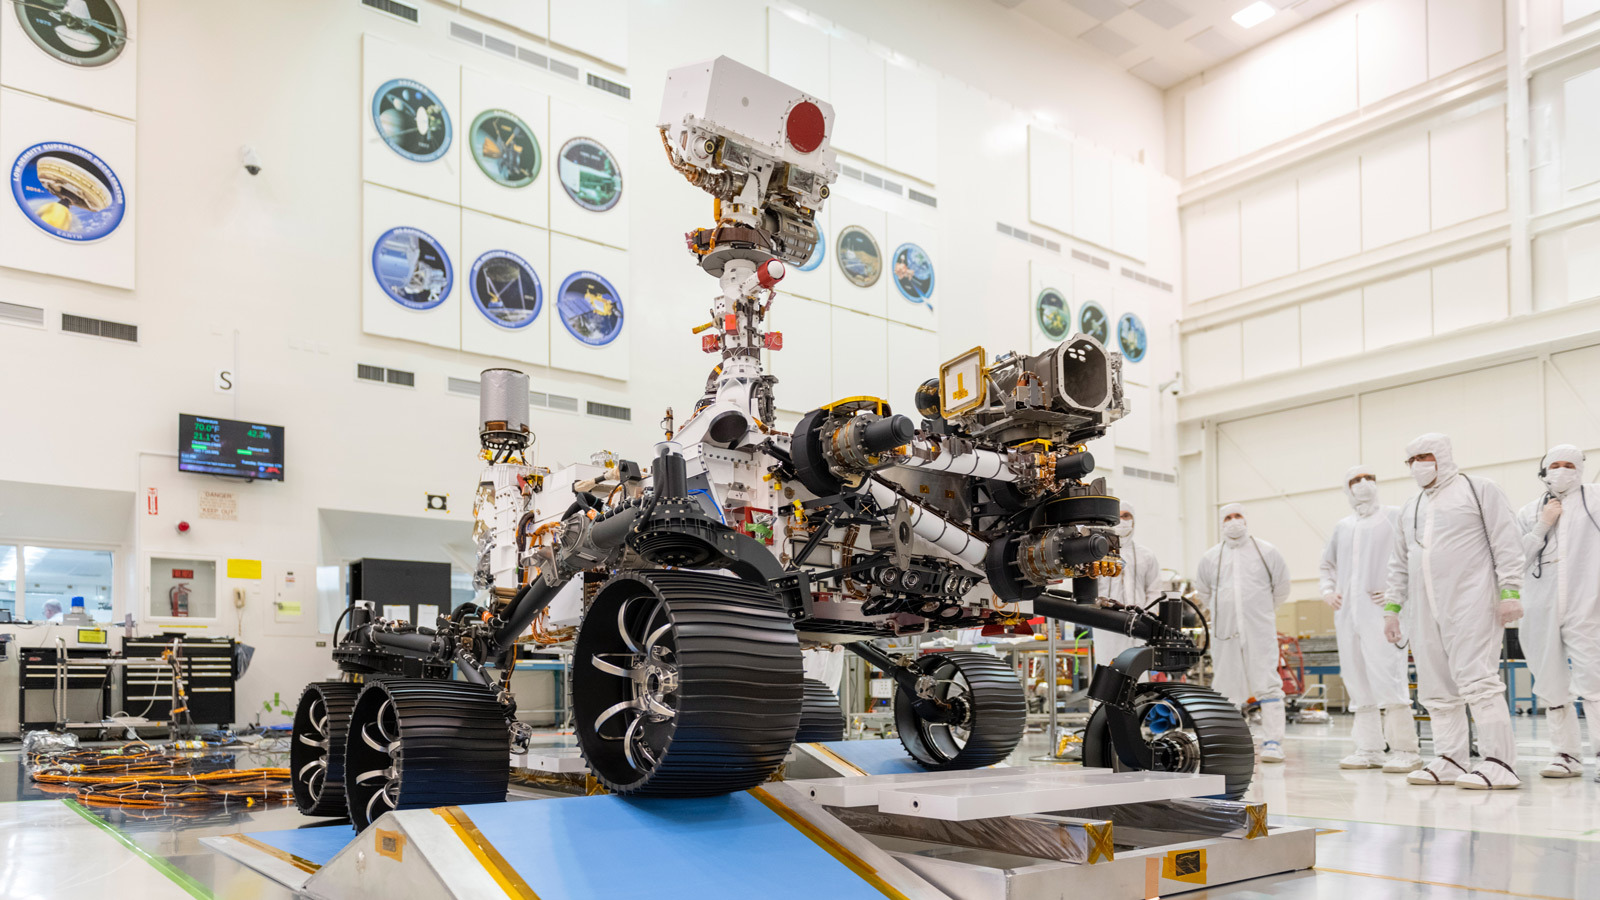
\includegraphics[height=9.5cm,keepaspectratio]{figures/perseverance.jpg}
  \end{figure}
\end{frame}

\begin{frame}[plain]
  % Instead, the rover uses an engineered navigation algorithm, or is even controlled directly by humans. (pause)
  % As an environment, Mars offers unique challenges.
  % For example, rocks can puncture the rover's wheels and sand can trap the rover.
  % The rover relies on a combination of on-board and satellite based sensor data, which is often imperfect.
  % Also, low-latency direct human control is impossible.
  \begin{figure}
  \centering
  \vspace*{-1em}
  \hspace*{-3em}
  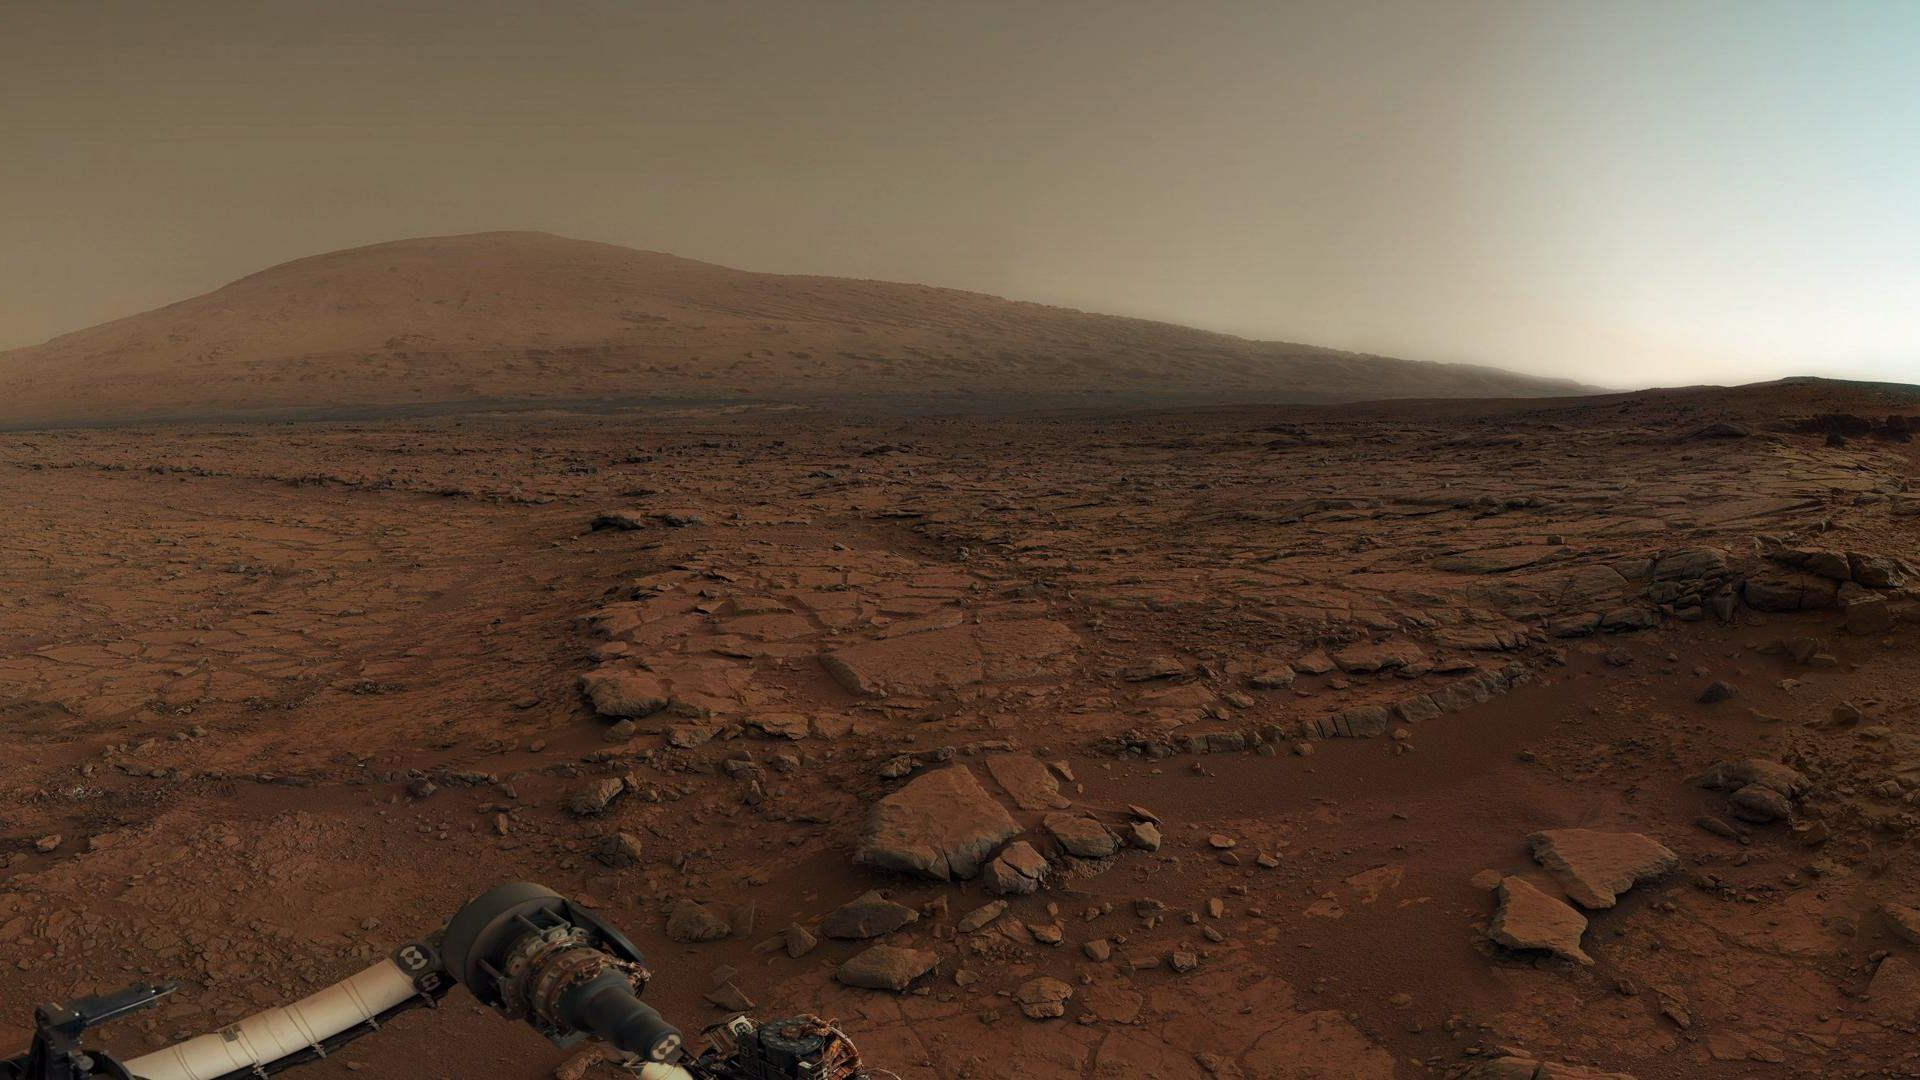
\includegraphics[height=9.5cm,keepaspectratio]{figures/mars_surface.jpg}
  \end{figure}
\end{frame}

\begin{frame}[plain]
  % Alternatively, consider an environment like an Amazon warehouse.
  % In contrast to mars, it is easy to navigate.
  % The floor is perfectly smooth, the environment is mapped almost perfectly.
  % Communication is fast, and it is easier integrate advanced machine learning algorithms with robots.
  % However, in an environment like this, there can be multiple robots, or even human-robot interaction.
  % Humans, unlike robots, don't broadcast their telemetry, and can be unpredictable.
  % So, robots must plan very carefully to avoid dangerous collisions.
  % (pause)
  % Considering these differences between Mars and an Amazon warehouse brings us to the main goal of this thesis.
  \begin{figure}
  \centering
  \vspace*{-1em}
  \hspace*{-3em}
  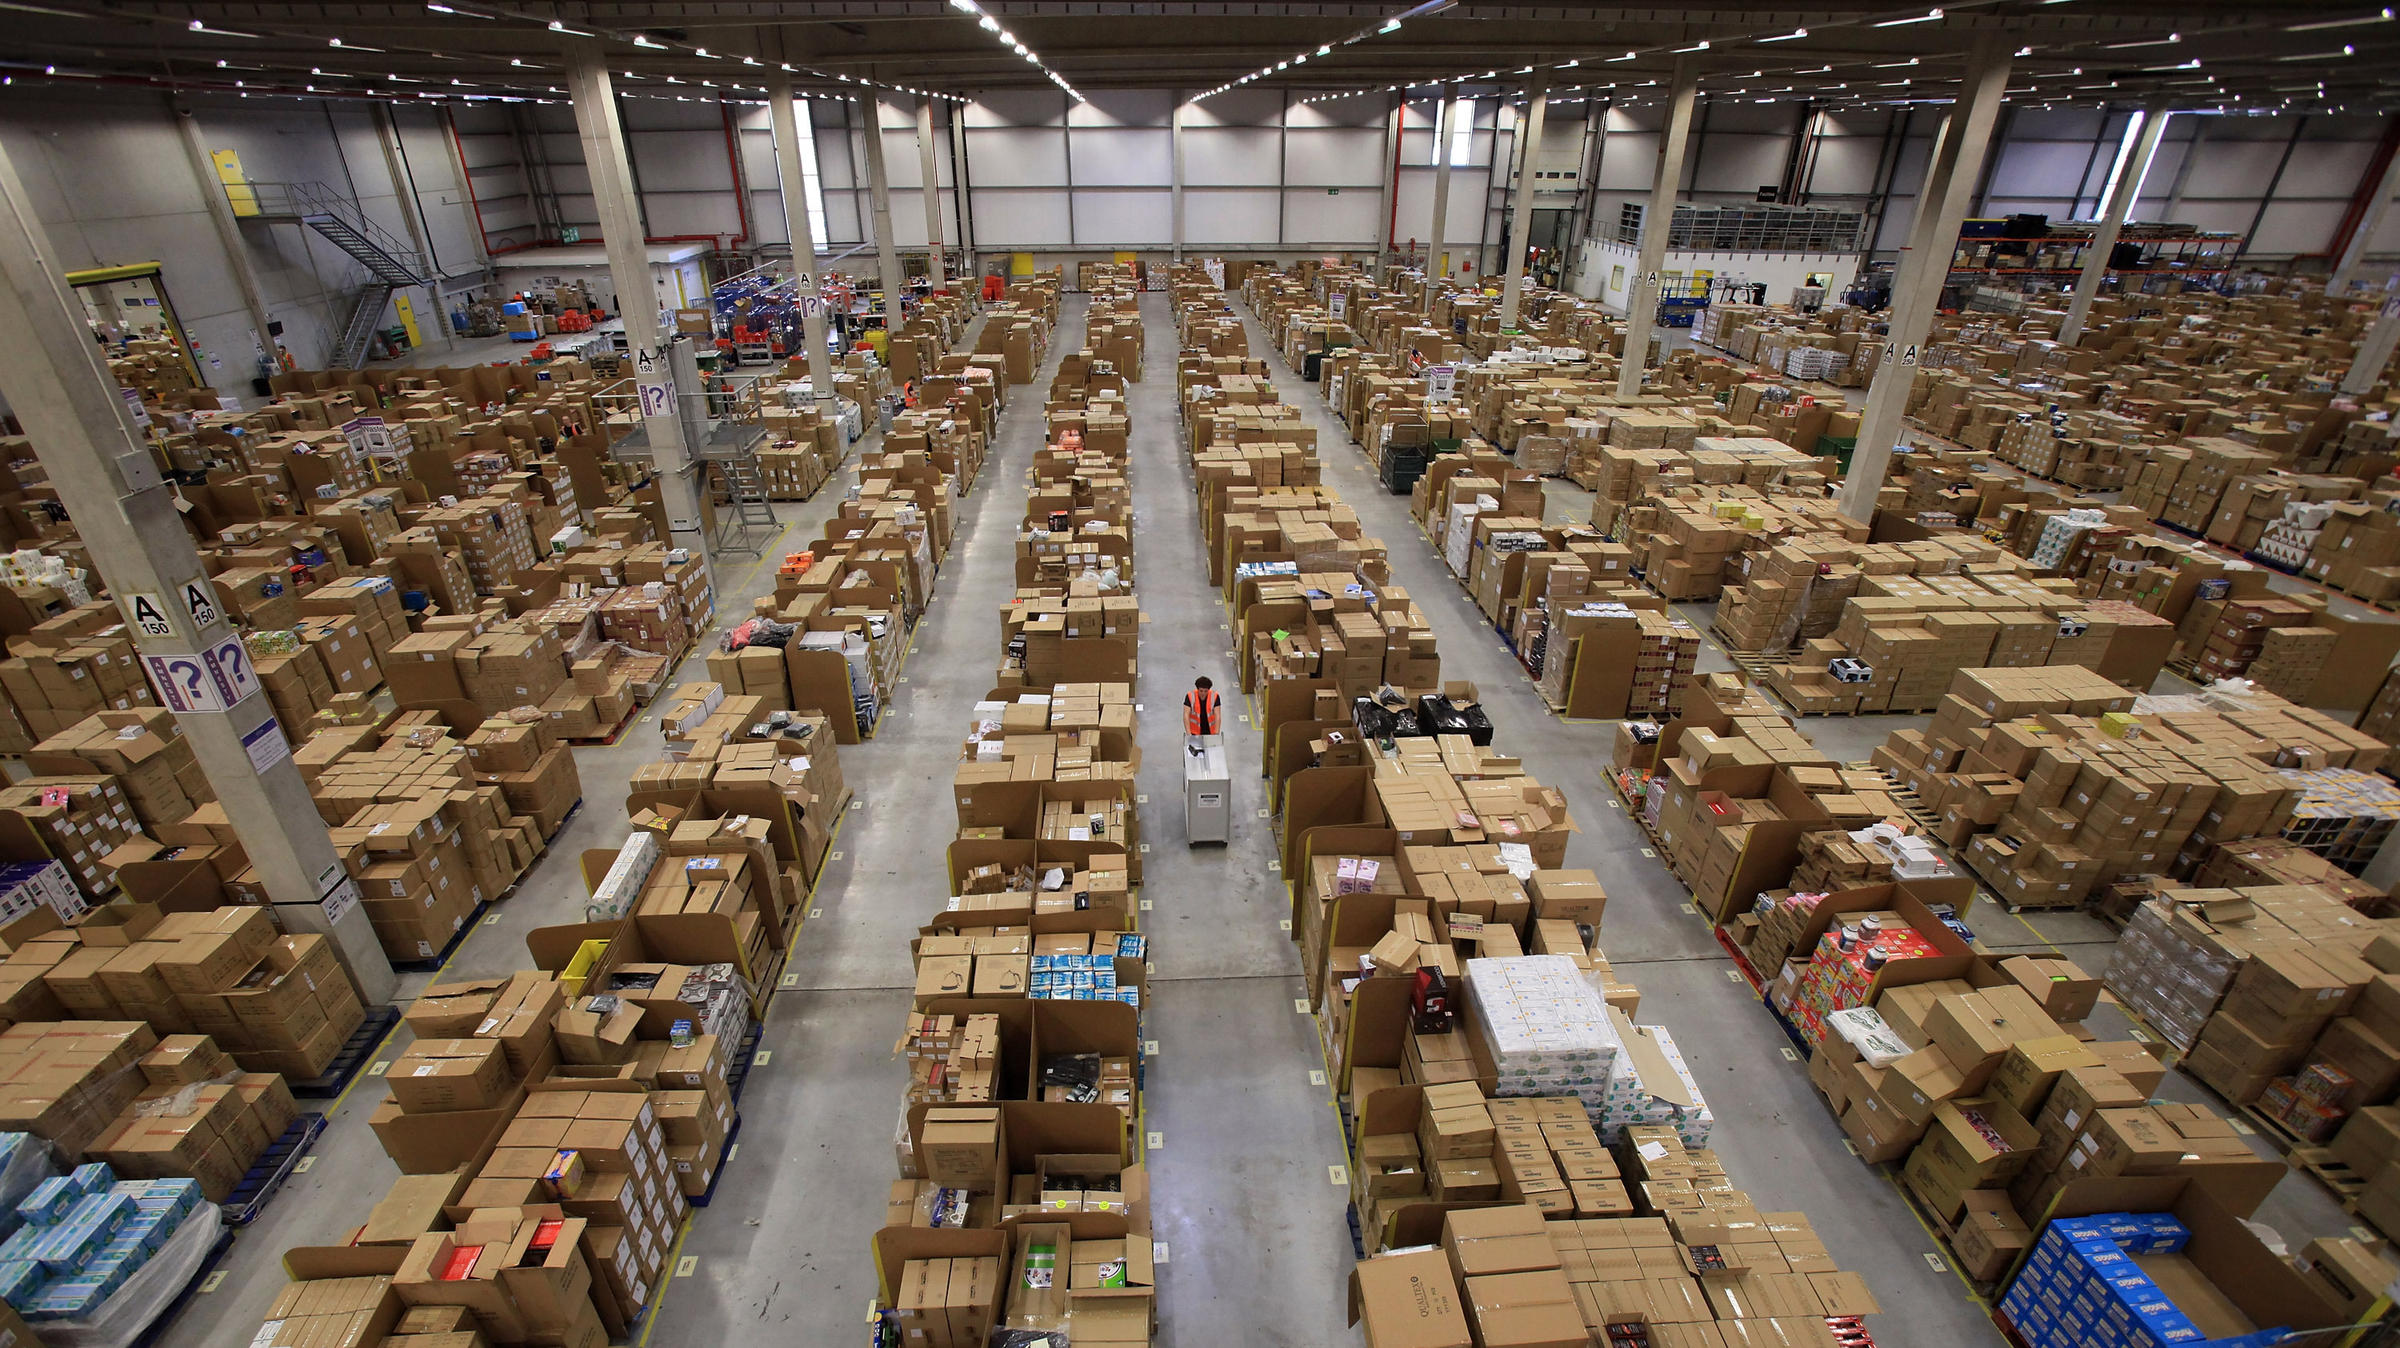
\includegraphics[height=9.5cm,keepaspectratio]{figures/warehouse.jpg}
  \end{figure}
\end{frame}

\begin{frame}{\white{Core Goals \& Concepts}}
  % Conceptually, the focus of this thesis is on life-long robot learning.
  %     Modern artificial intelligence is trying to move away from custom-engineering
  %     In the context of this paper, this means teaching robots to be generally proficient.
  %     But most importantly, this thesis focuses on the potential to specialize robots to particular environments.
  % (pause)
  % On the right, we have an image which I think is quite beautiful.
  % This is a sketch from Darwin's notebook, presumably from when he first thought of evolution.
  % It shows a tree depicting common ancestry and specialization.
  \begin{columns}[T]
      \begin{column}{.5\linewidth}
            \vspace{-0.7em}
            \emph{Learning}
            \begin{itemize}
              \item {\Medium Flexibility: adapt to new tasks}
            \end{itemize}
            \vspace{1em}
            \emph{Generalization}
            \begin{itemize}
              \item {\Medium Learn overall task proficiency?}
            \end{itemize}
            \vspace{1em}
            \emph{Specialization}
            \begin{itemize}
              \item {\Medium Learn environment details?}
            \end{itemize}
      \end{column}
      \begin{column}{.5\linewidth}
          \begin{figure}
              \centering
              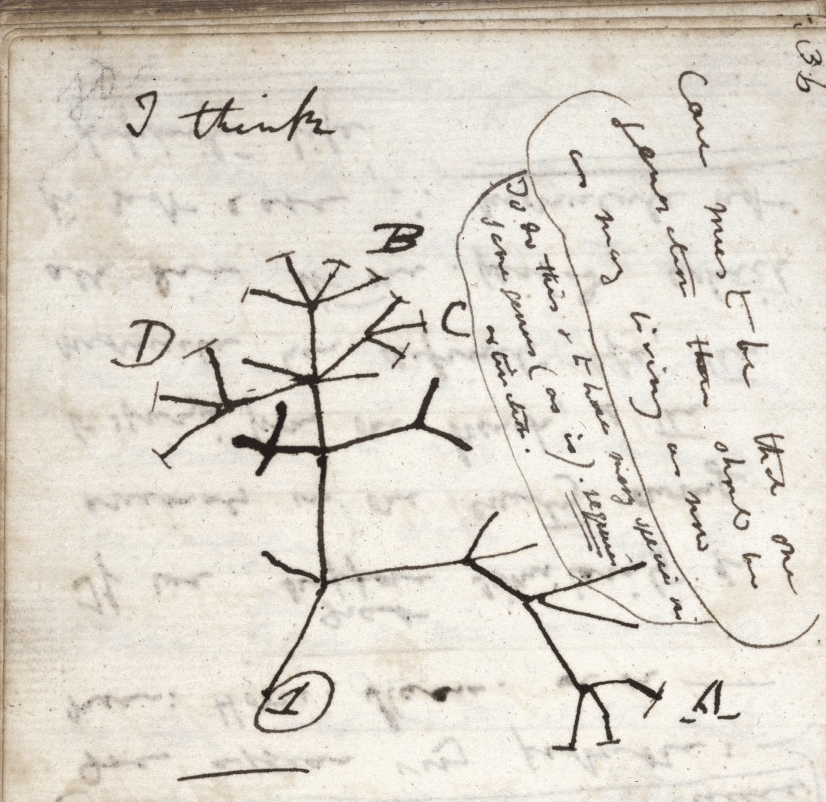
\includegraphics[height=5.5cm, keepaspectratio]{figures/i_think.png}
              \caption{Where is this image from?}
              \label{fig:i_think}
          \end{figure}
      \end{column}
  \end{columns}
\end{frame}

{
\setbeamercolor{background canvas}{bg=white}
\begin{frame}[plain]
  % This is an artist's depiction of the tree of life,
  % In particular, it shows how specialization occurred over time.
  % Bacteria have the oldest common ancestry.
  % Mammals, on the other hand, are the most recent, and fill a vastly different niche.
  % In between, there are incredibly diverse species of plants, fungi, fish, reptiles, and birds.
  % This has led to at least 8.7 million species on earth
  \begin{figure}
  \centering
  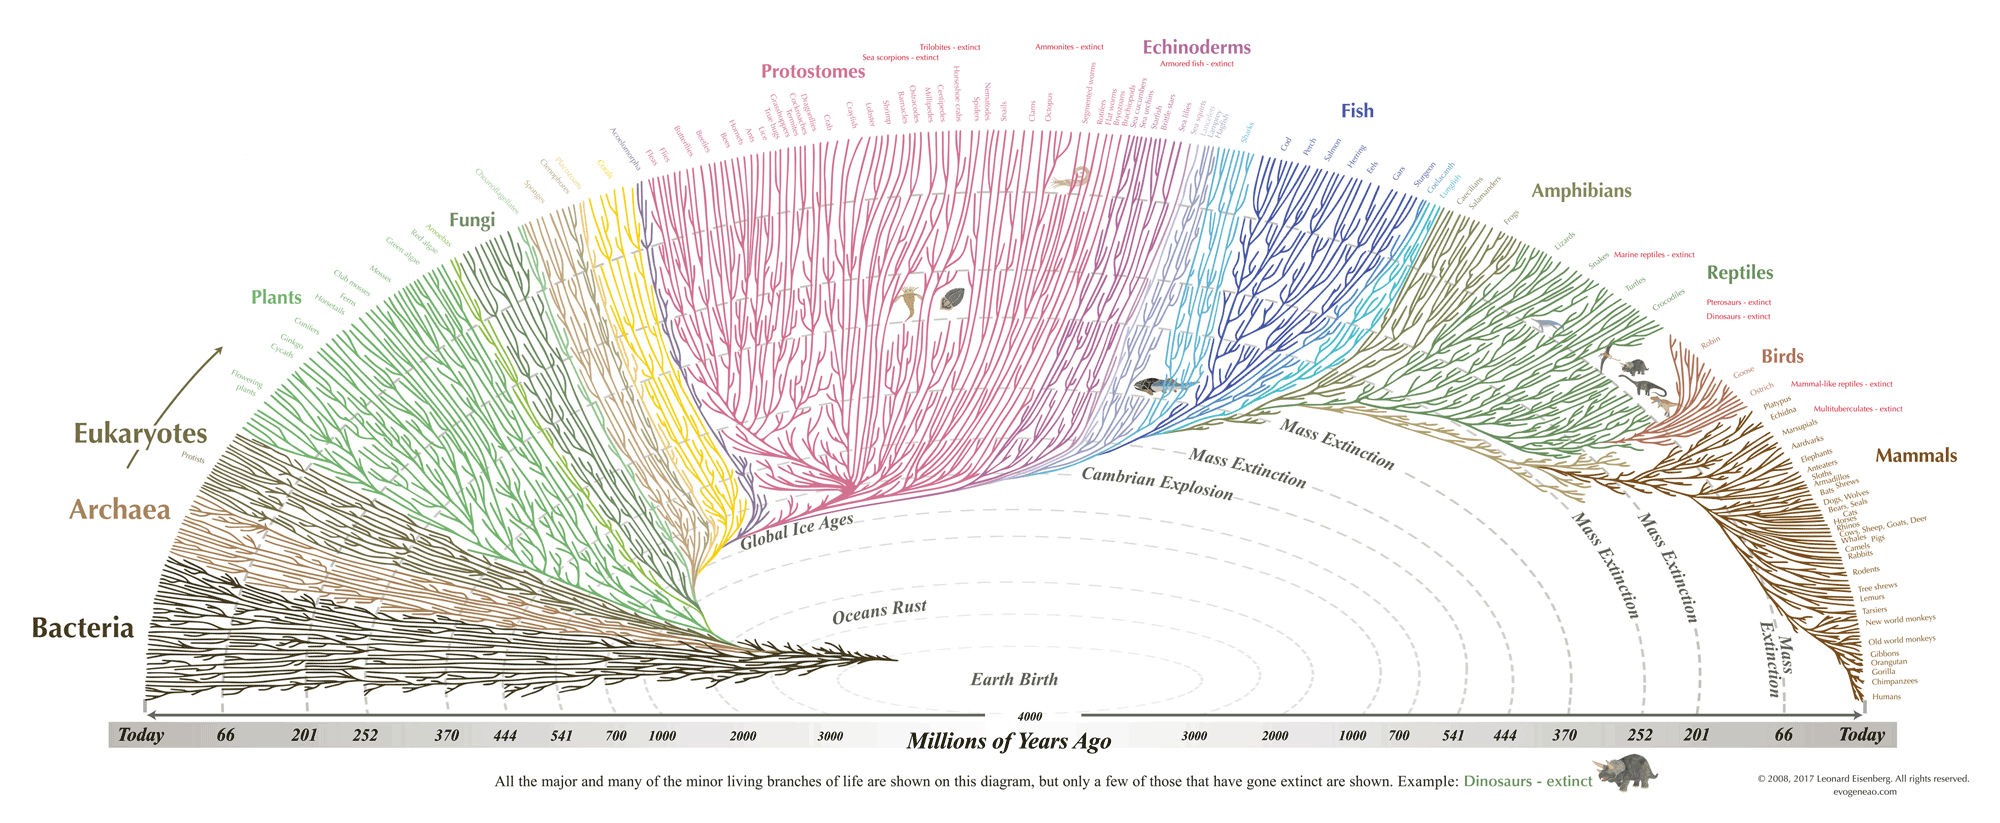
\includegraphics[width=1.0\linewidth,keepaspectratio]{figures/tree_of_life.png}
  \end{figure}
  \begin{center}
      \emph{Natural evolution}
  \end{center}
\end{frame}
}

\begin{frame}[plain]
  % Ideally, this thesis would achieve the same specialization, but with robots instead of biological species.
  % In this slide is a teaser figure showing an ancestry tree approximating that of natural species.
  \begin{figure}
  \centering
  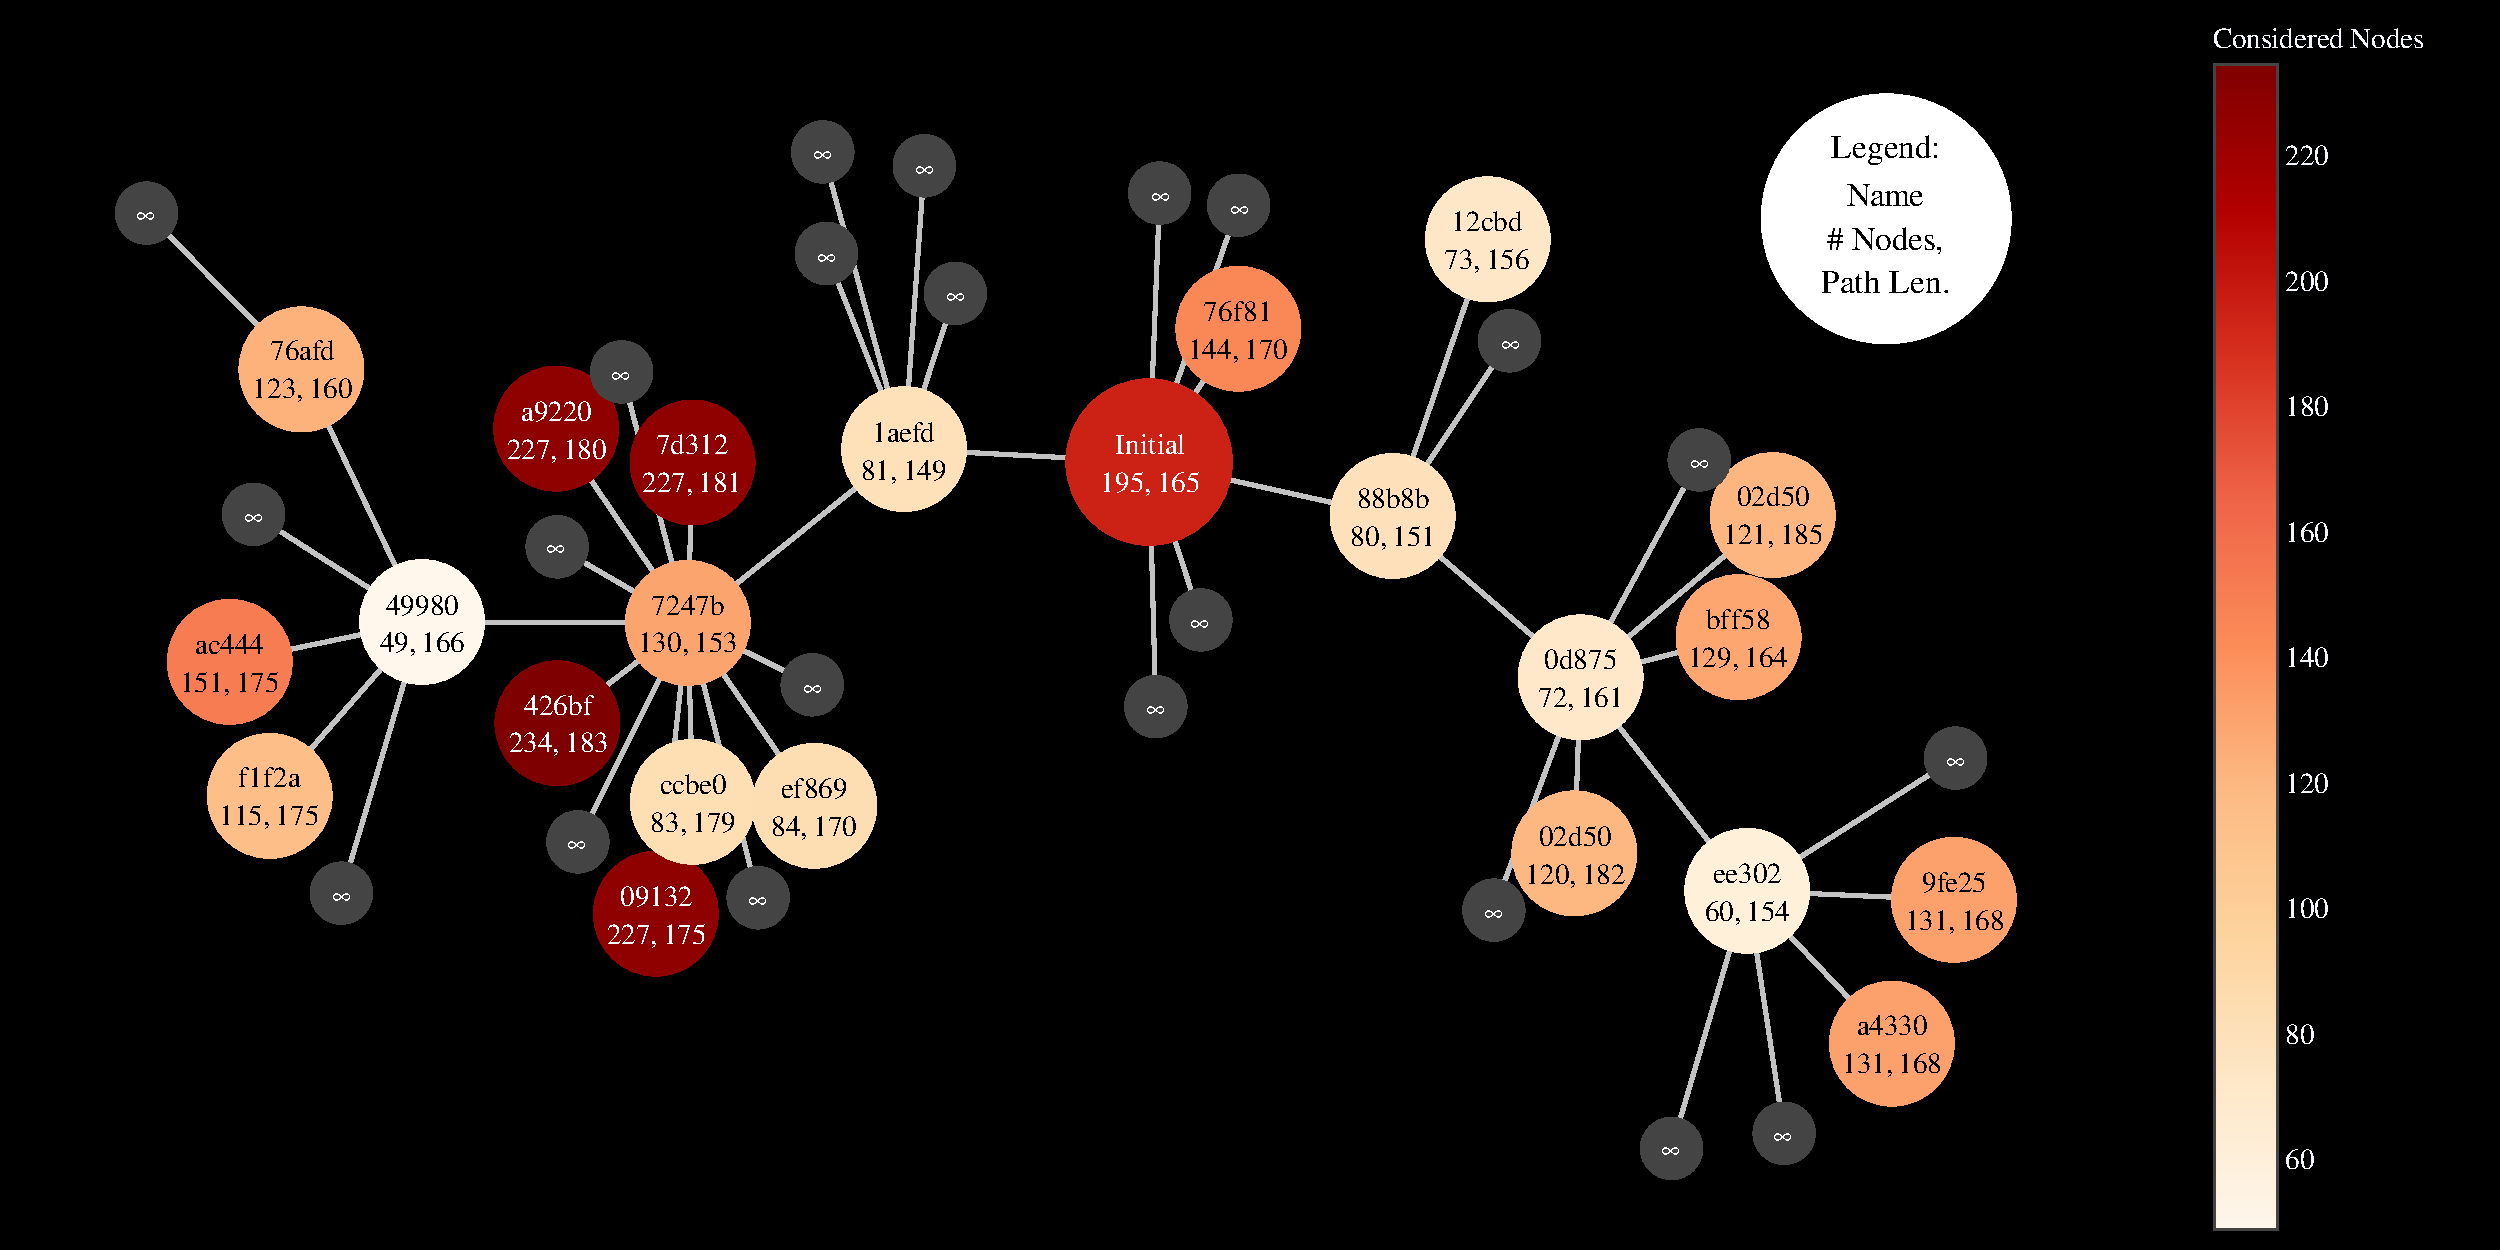
\includegraphics[width=1.0\linewidth,keepaspectratio]{figures/tree.pdf}
  \end{figure}
  \begin{center}
  \emph{Evolved Computer Programs}
  \end{center}
\end{frame}

\begin{frame}[plain]{}
  \centering
  \vfill
  \red{\fontsize{40}{50}\selectfont Computer Programs instead of species}
  \vfill
  \Huge Evolutionary Programming
\end{frame}

\begin{frame}[plain]{\white{Problems Considered}}
  % The types of computer programs that we consider are *Path Planners*
  % Path planning is the task of finding a sequence of moves between points in space.
  % For example, on the left is a 2 dimensional map of Milan, Italy, and a robot has been tasked with finding a path between the Orange dot and the Purple dot.
  % Originally, this thesis focused on graph-based planning, where possible moves are specified in advance.
  % However, it has moved towards sampling-based planning, where possible moves are gathered by probing the environment.
  % The methods describes in this thesis work just as well dynamic (Mars) or multi-agent planning (Amazon), but these are left for future work. 
  % They also have strong relations to symbolic regression or neural architecture search.
  \begin{columns}[T]
      \begin{column}{.5\linewidth}
          \vspace{0.5cm}
          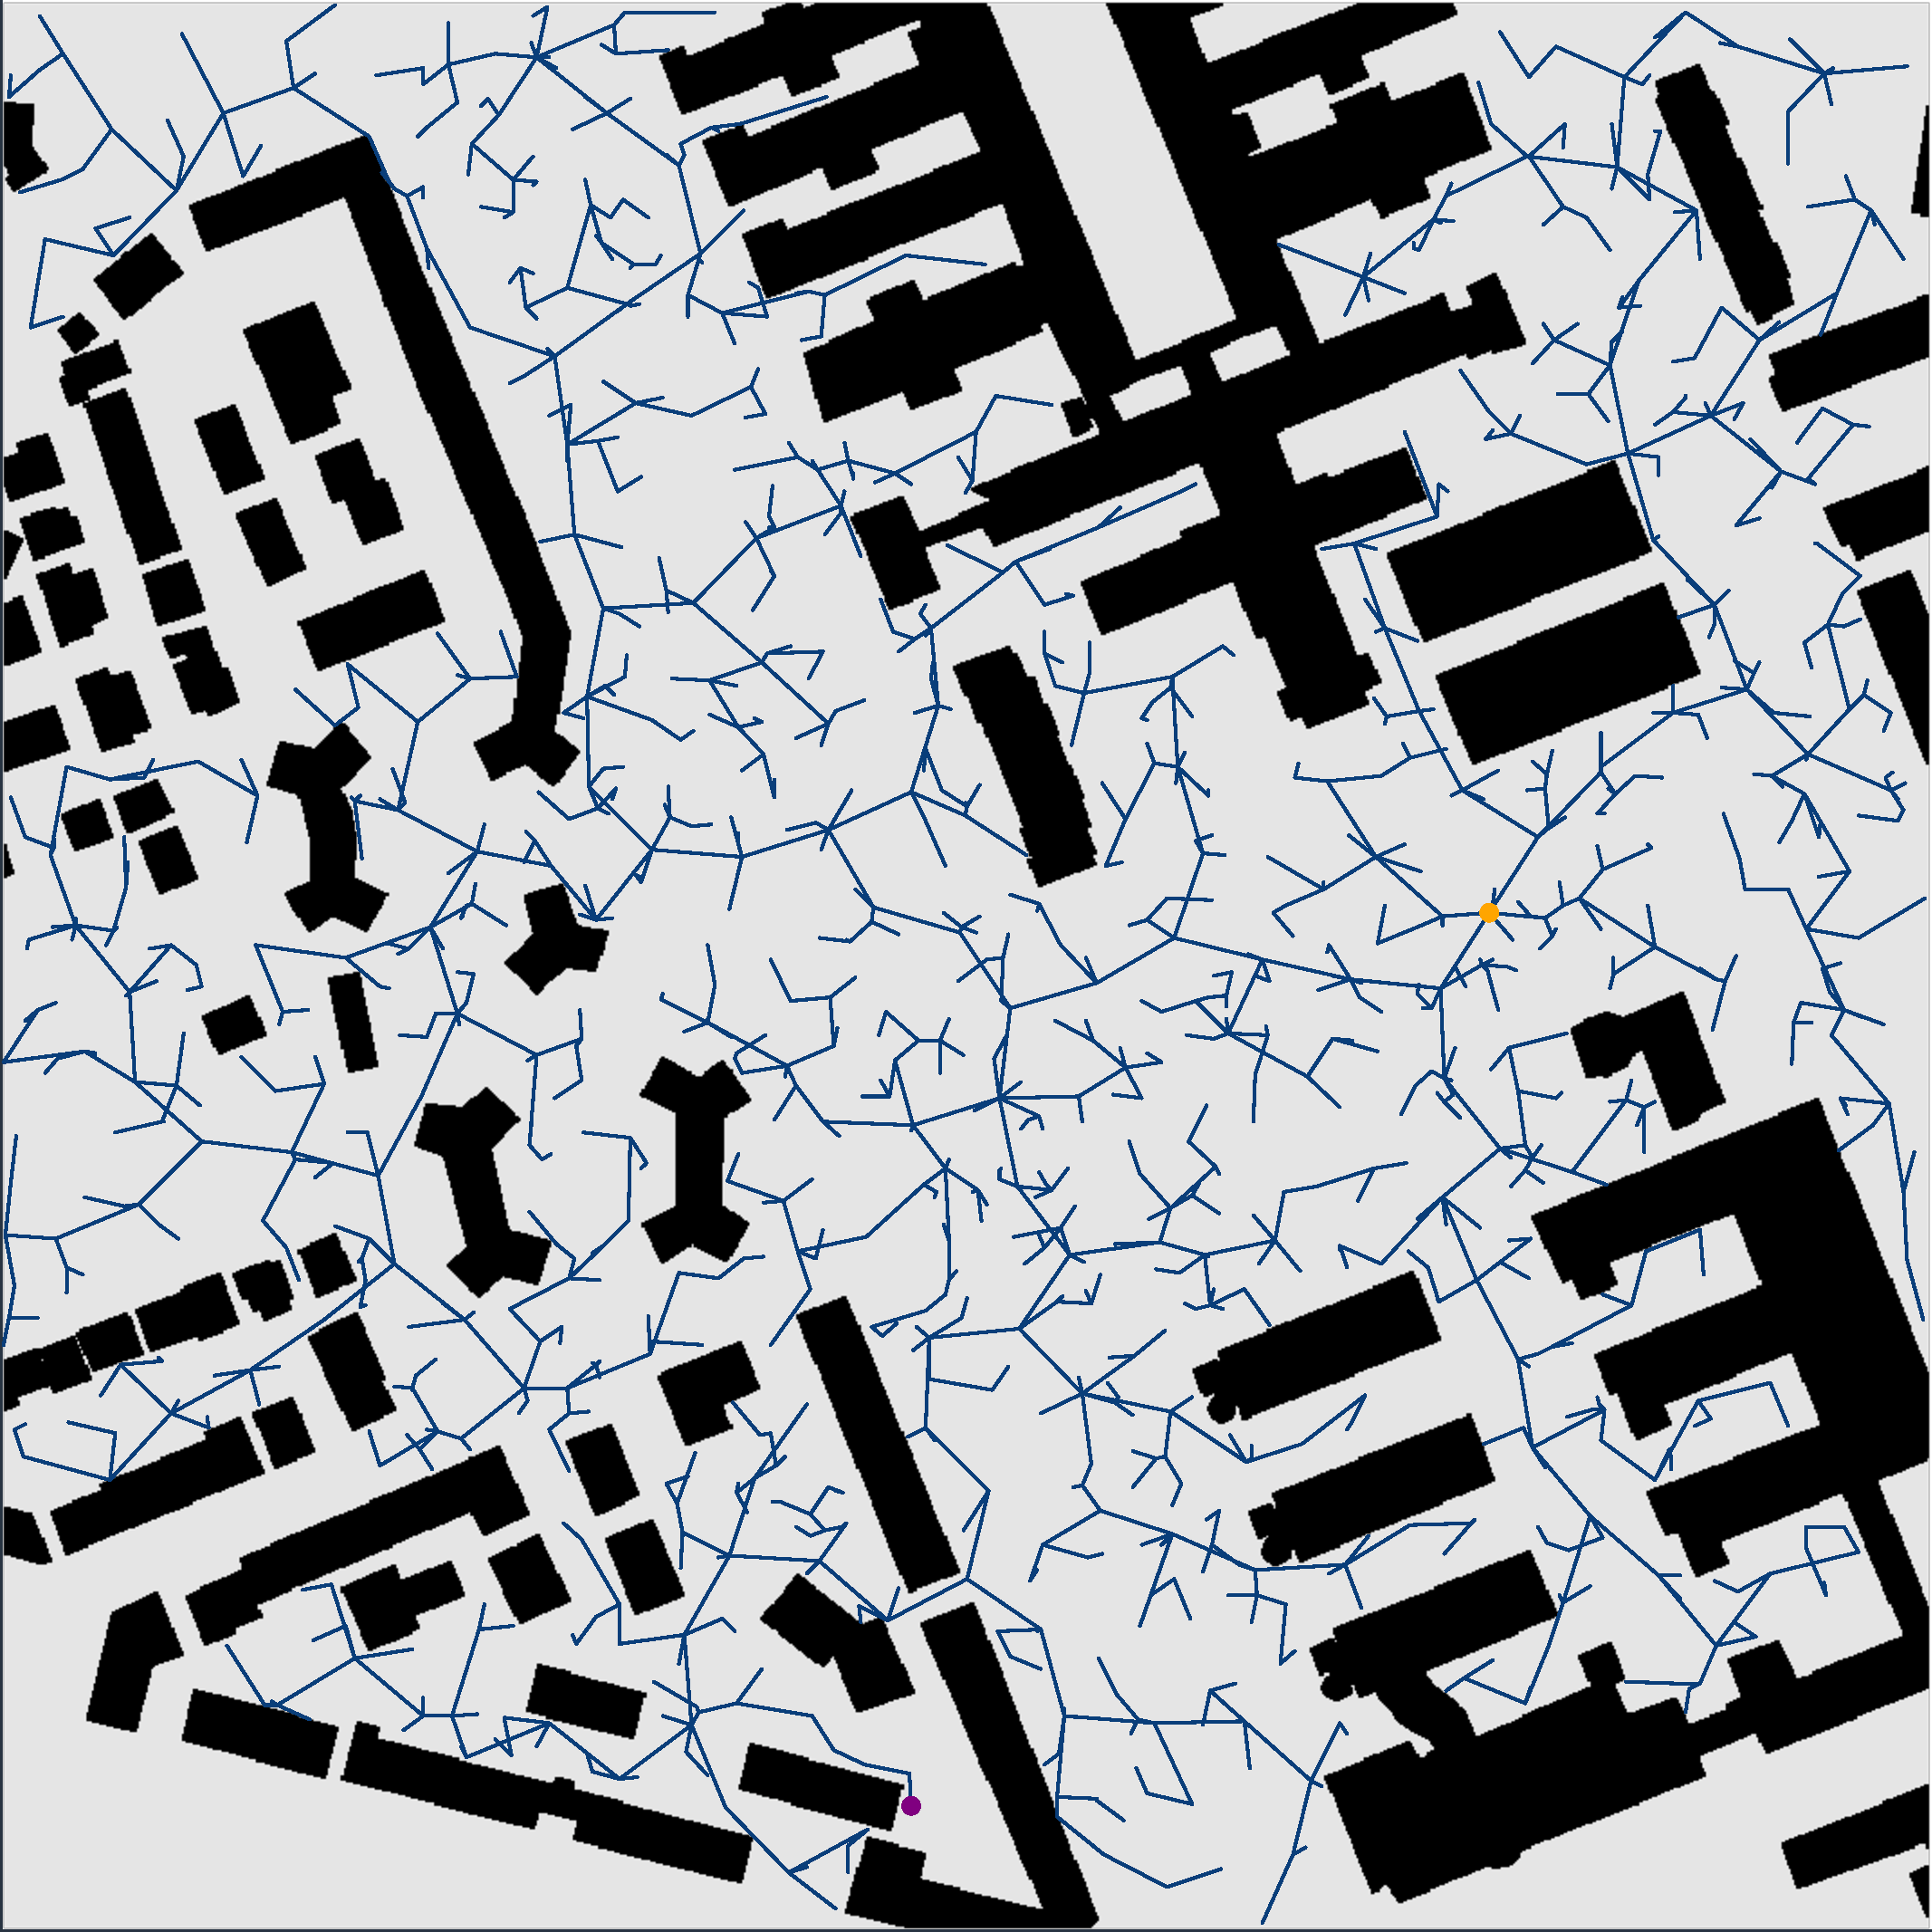
\includegraphics[width=1.0\linewidth, keepaspectratio]{figures/one_off.pdf}
          \vfill
      \end{column}
      \hspace{1.0em}
      \begin{column}{.5\linewidth}
          \emph{Path Planning}
          \begin{vfilleditems}
              \item {\Large Graph-based}
              \vspace{1em}
              \item {\Large Sample-based \Medium (left)}
              \vspace{1em}
              \item {\color{grey} {\Large Dynamic (i.e. Mars)}}
              \vspace{1em}
              \item {\color{grey} {\Large Multi-agent (i.e. Amazon)}}
          \end{vfilleditems}
          \vspace{1em}
          {\color{grey} {\Large Symbolic Regression}}
          \vspace{1em}
          {\color{grey} {\Large Neural Arch. Search}}
      \end{column}
  \end{columns}
\end{frame}

\begin{frame}[plain]{Graph search w/ Dijkstra \white{(New York)}}
    % This image shows the behavior of a graph-based path planner, specifically Dijkstra's algorithm, on a map of New York.
    % In this case, the streets are specified in advance, and a planning algorithm is asked to find a route from the bottom of New York to the top of New York
    % Pink indicates roads that were considered
    % Blank indicates unconsidered roads
    % Yellow indicates the optimal path
    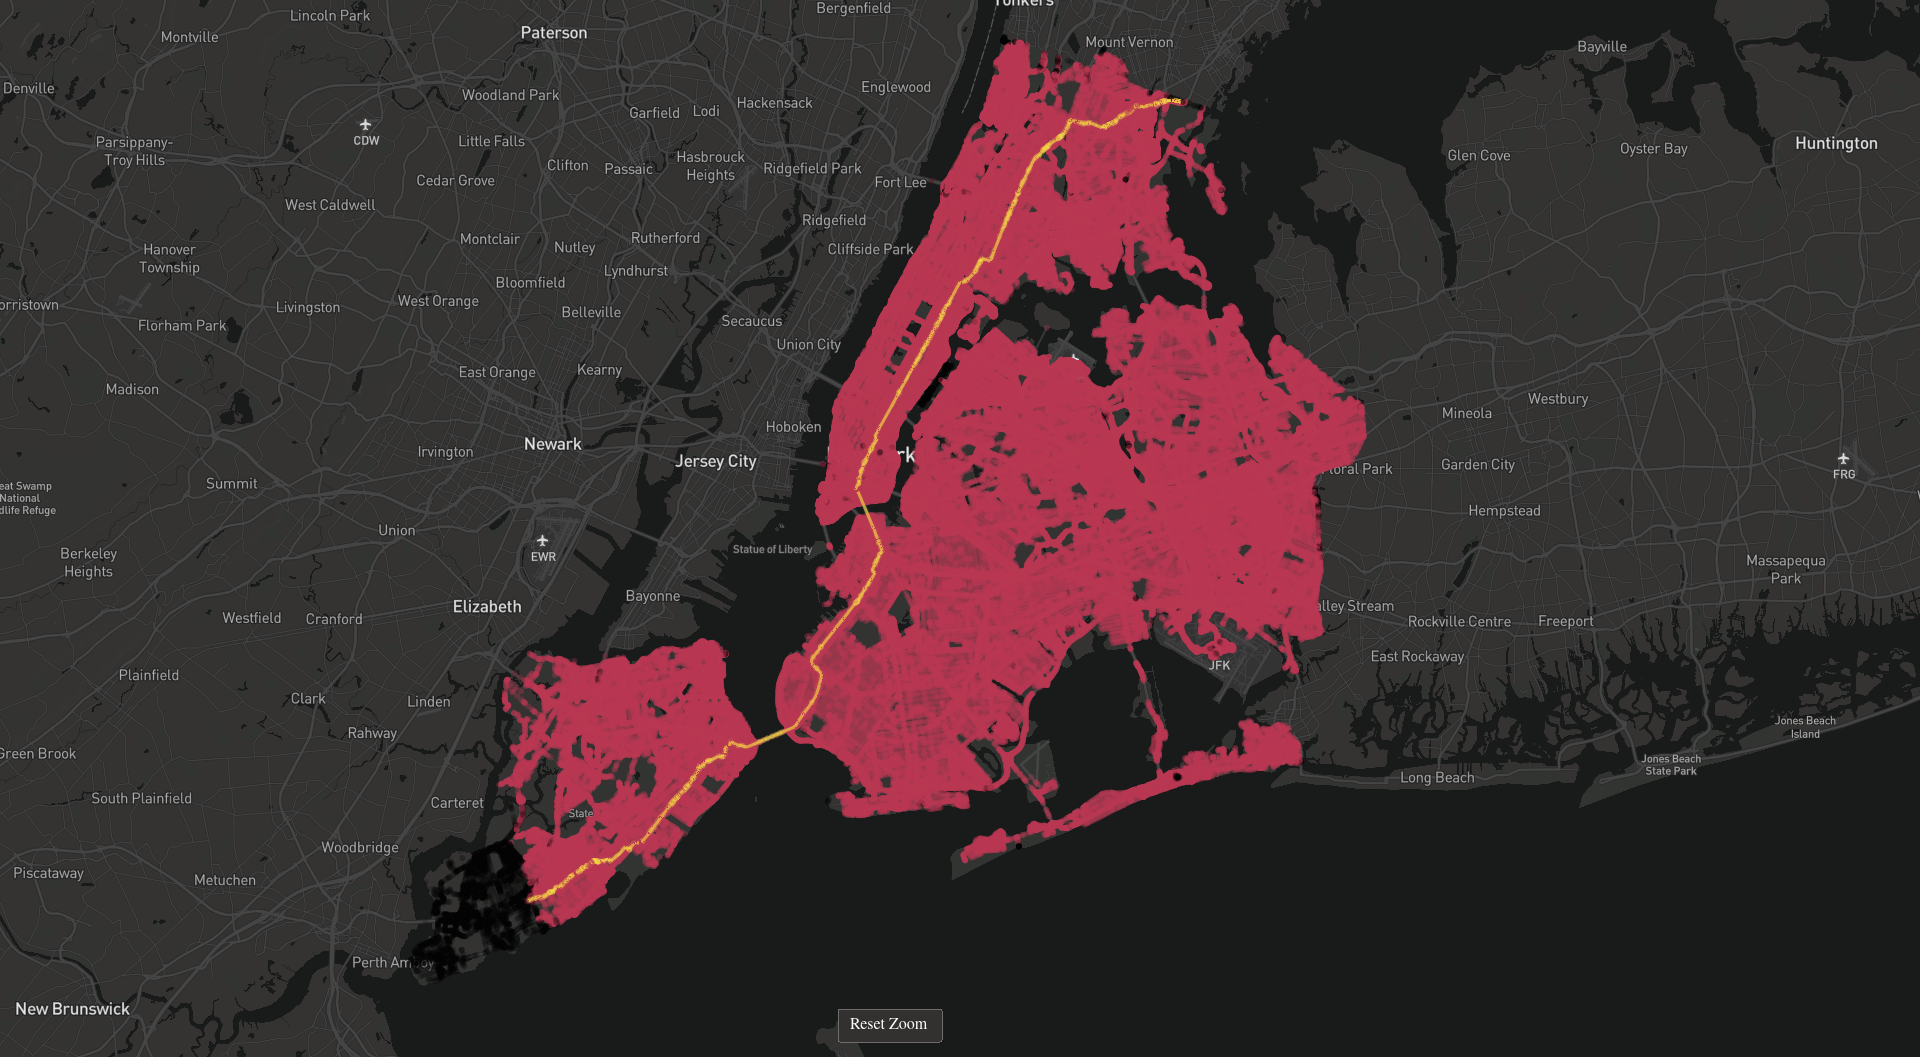
\includegraphics[width=1.0\linewidth, keepaspectratio, trim={0cm, 2cm, 1cm, 0.5cm}, clip]{figures/ny_graph_based.png}
\end{frame}

\begin{frame}[plain]{Graph search w/ A* \white{(New York)}}
    % However, the choice of algorithm can be a difference of millions of nodes
    % This algorithm is A* with a geodesic heuristic, i.e. with knowledge about how far from the goal each road is.
    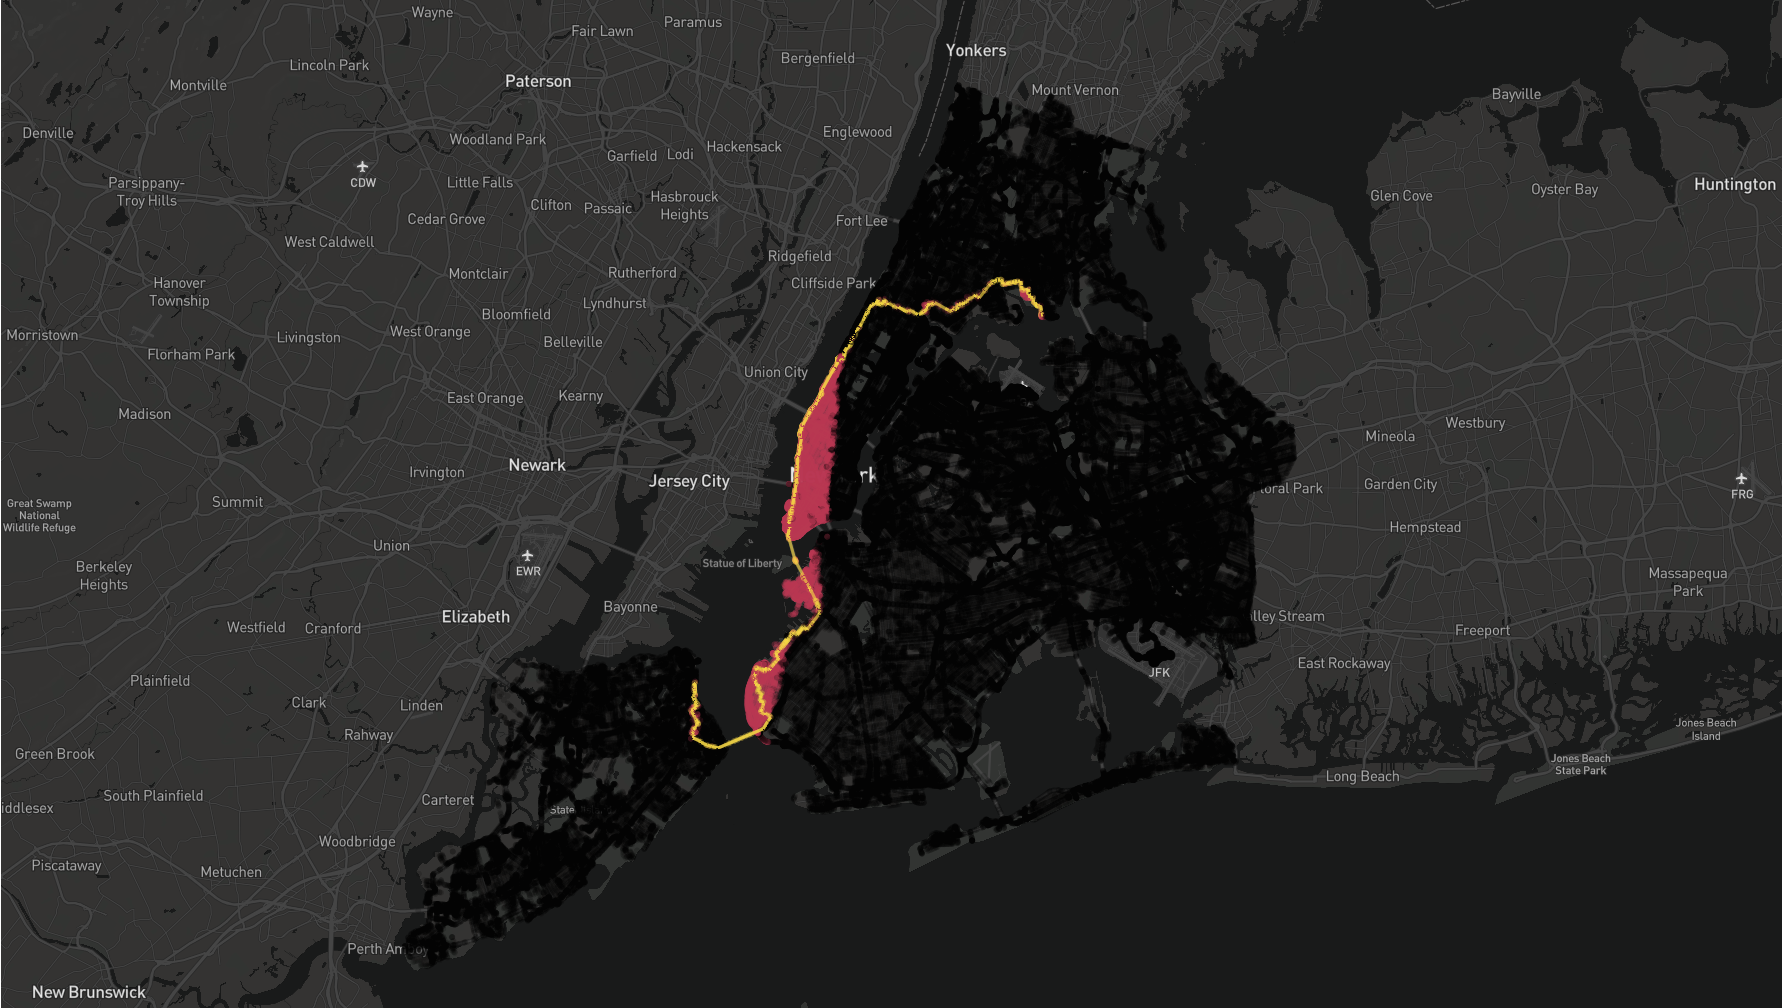
\includegraphics[width=1.0\linewidth, keepaspectratio, trim={0.5cm 1.5cm 0 2.5cm}, clip]{figures/ny_graph_based_geodesic.png}
\end{frame}

\begin{frame}[plain]{Graph-based Algorithms \white{(Kiev, Ukraine)}}
  % In this thesis, I focus on four relatively simple algorithms.
  % These are Breadth first search, depth first search, Dijkstra's algorithm, and A* and its variants.
  % If people are interested in more advanced algorithms, Hannah Bast of the University of Frieberg has an amazing paper on the subject.
  % When using a service like Google Maps, it is more likely that it uses one of these more advanced algorithms.
  \begin{columns}[T]
      \begin{column}{.4\linewidth}
          \begin{vfilleditems}
              \item {\Large Breadth-first (BFS)}
              \item {\Large Depth-first (DFS)}
              \item {\Large Dijkstra/A*}
              \vspace{1em}
              {\color{grey}
              \item {\Large Goal-directed}
              \item {\Large Separator-based}
              \item {\Large Hierarchical}
              \item {\Large Bounded Hop}
              \item {\Large Hybrid Techniques}
              \vspace{1em}
              }
              \item \red{\Large \cite{bast2016route}}
          \end{vfilleditems}
      \end{column}
      \begin{column}{.6\linewidth}
      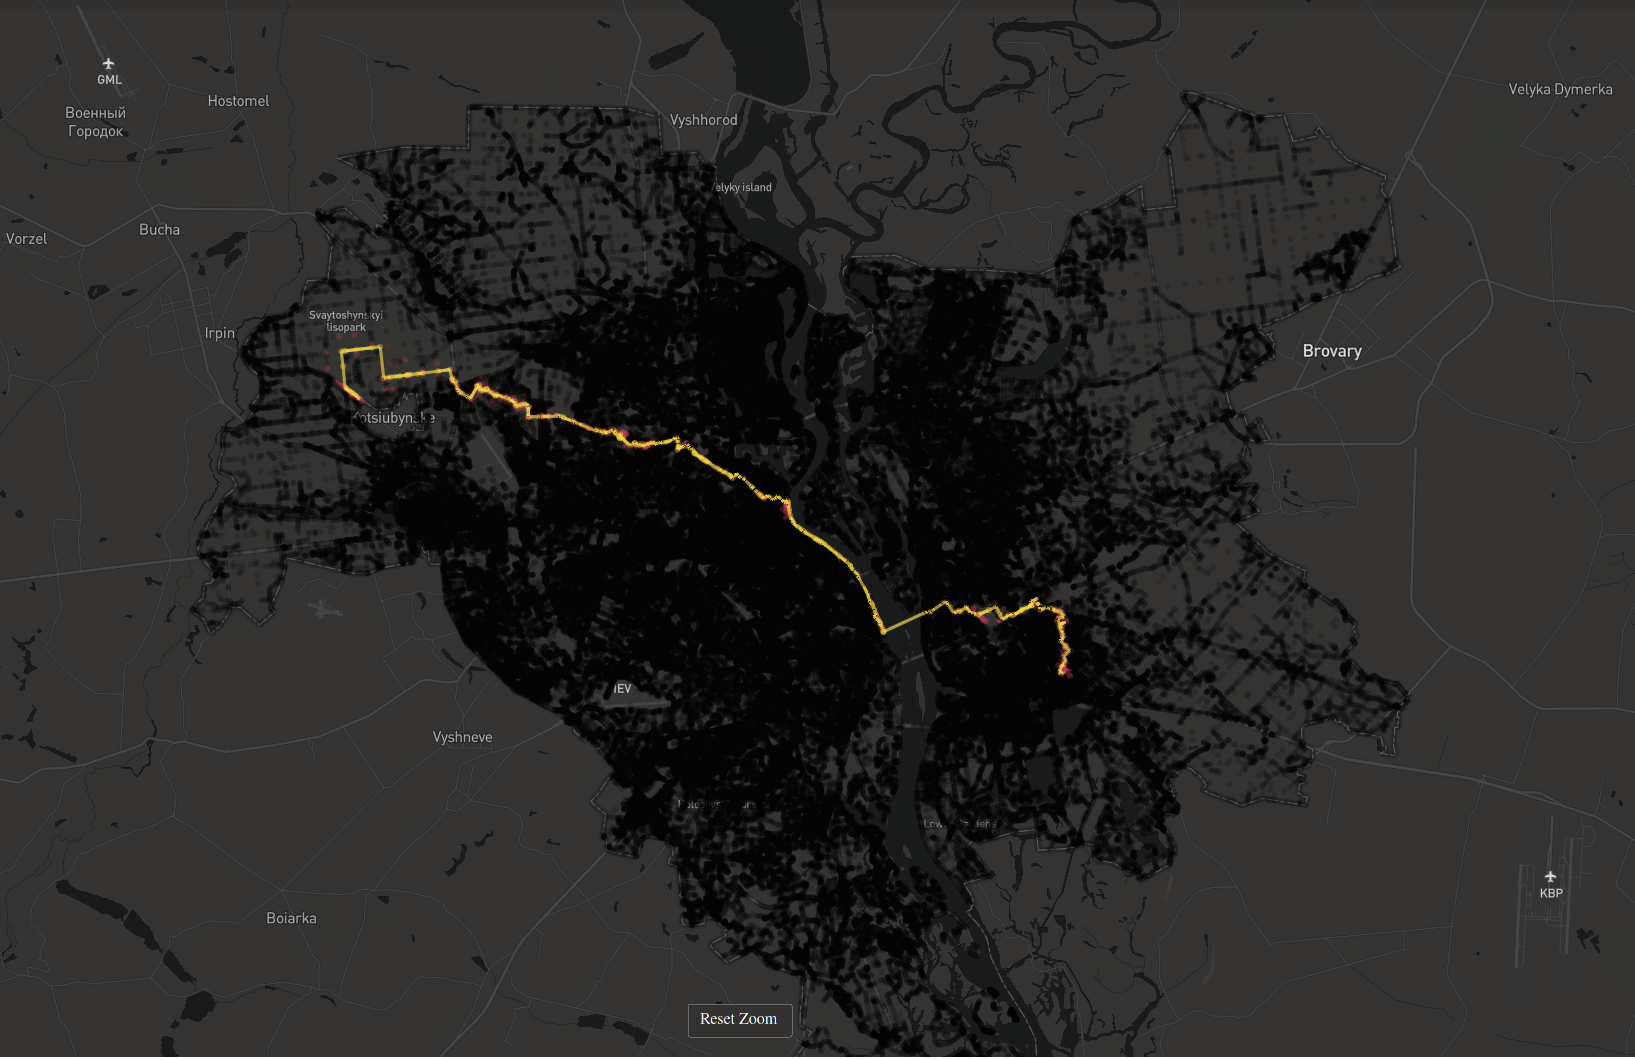
\includegraphics[height=0.9\textheight, keepaspectratio, trim={5cm 3cm 12cm 2cm}, clip]{figures/kiev.png}
      \end{column}
  \end{columns}
\end{frame}

\begin{frame}[plain]{Sampling-based search \white{(Baldur's Gate)}}
  % Next, there are sampling-based algorithms, which work by randomly selecting points in space.
  % 
  \begin{columns}[T]
      \begin{column}{.35\linewidth}
      \vspace{0.05\textheight}
      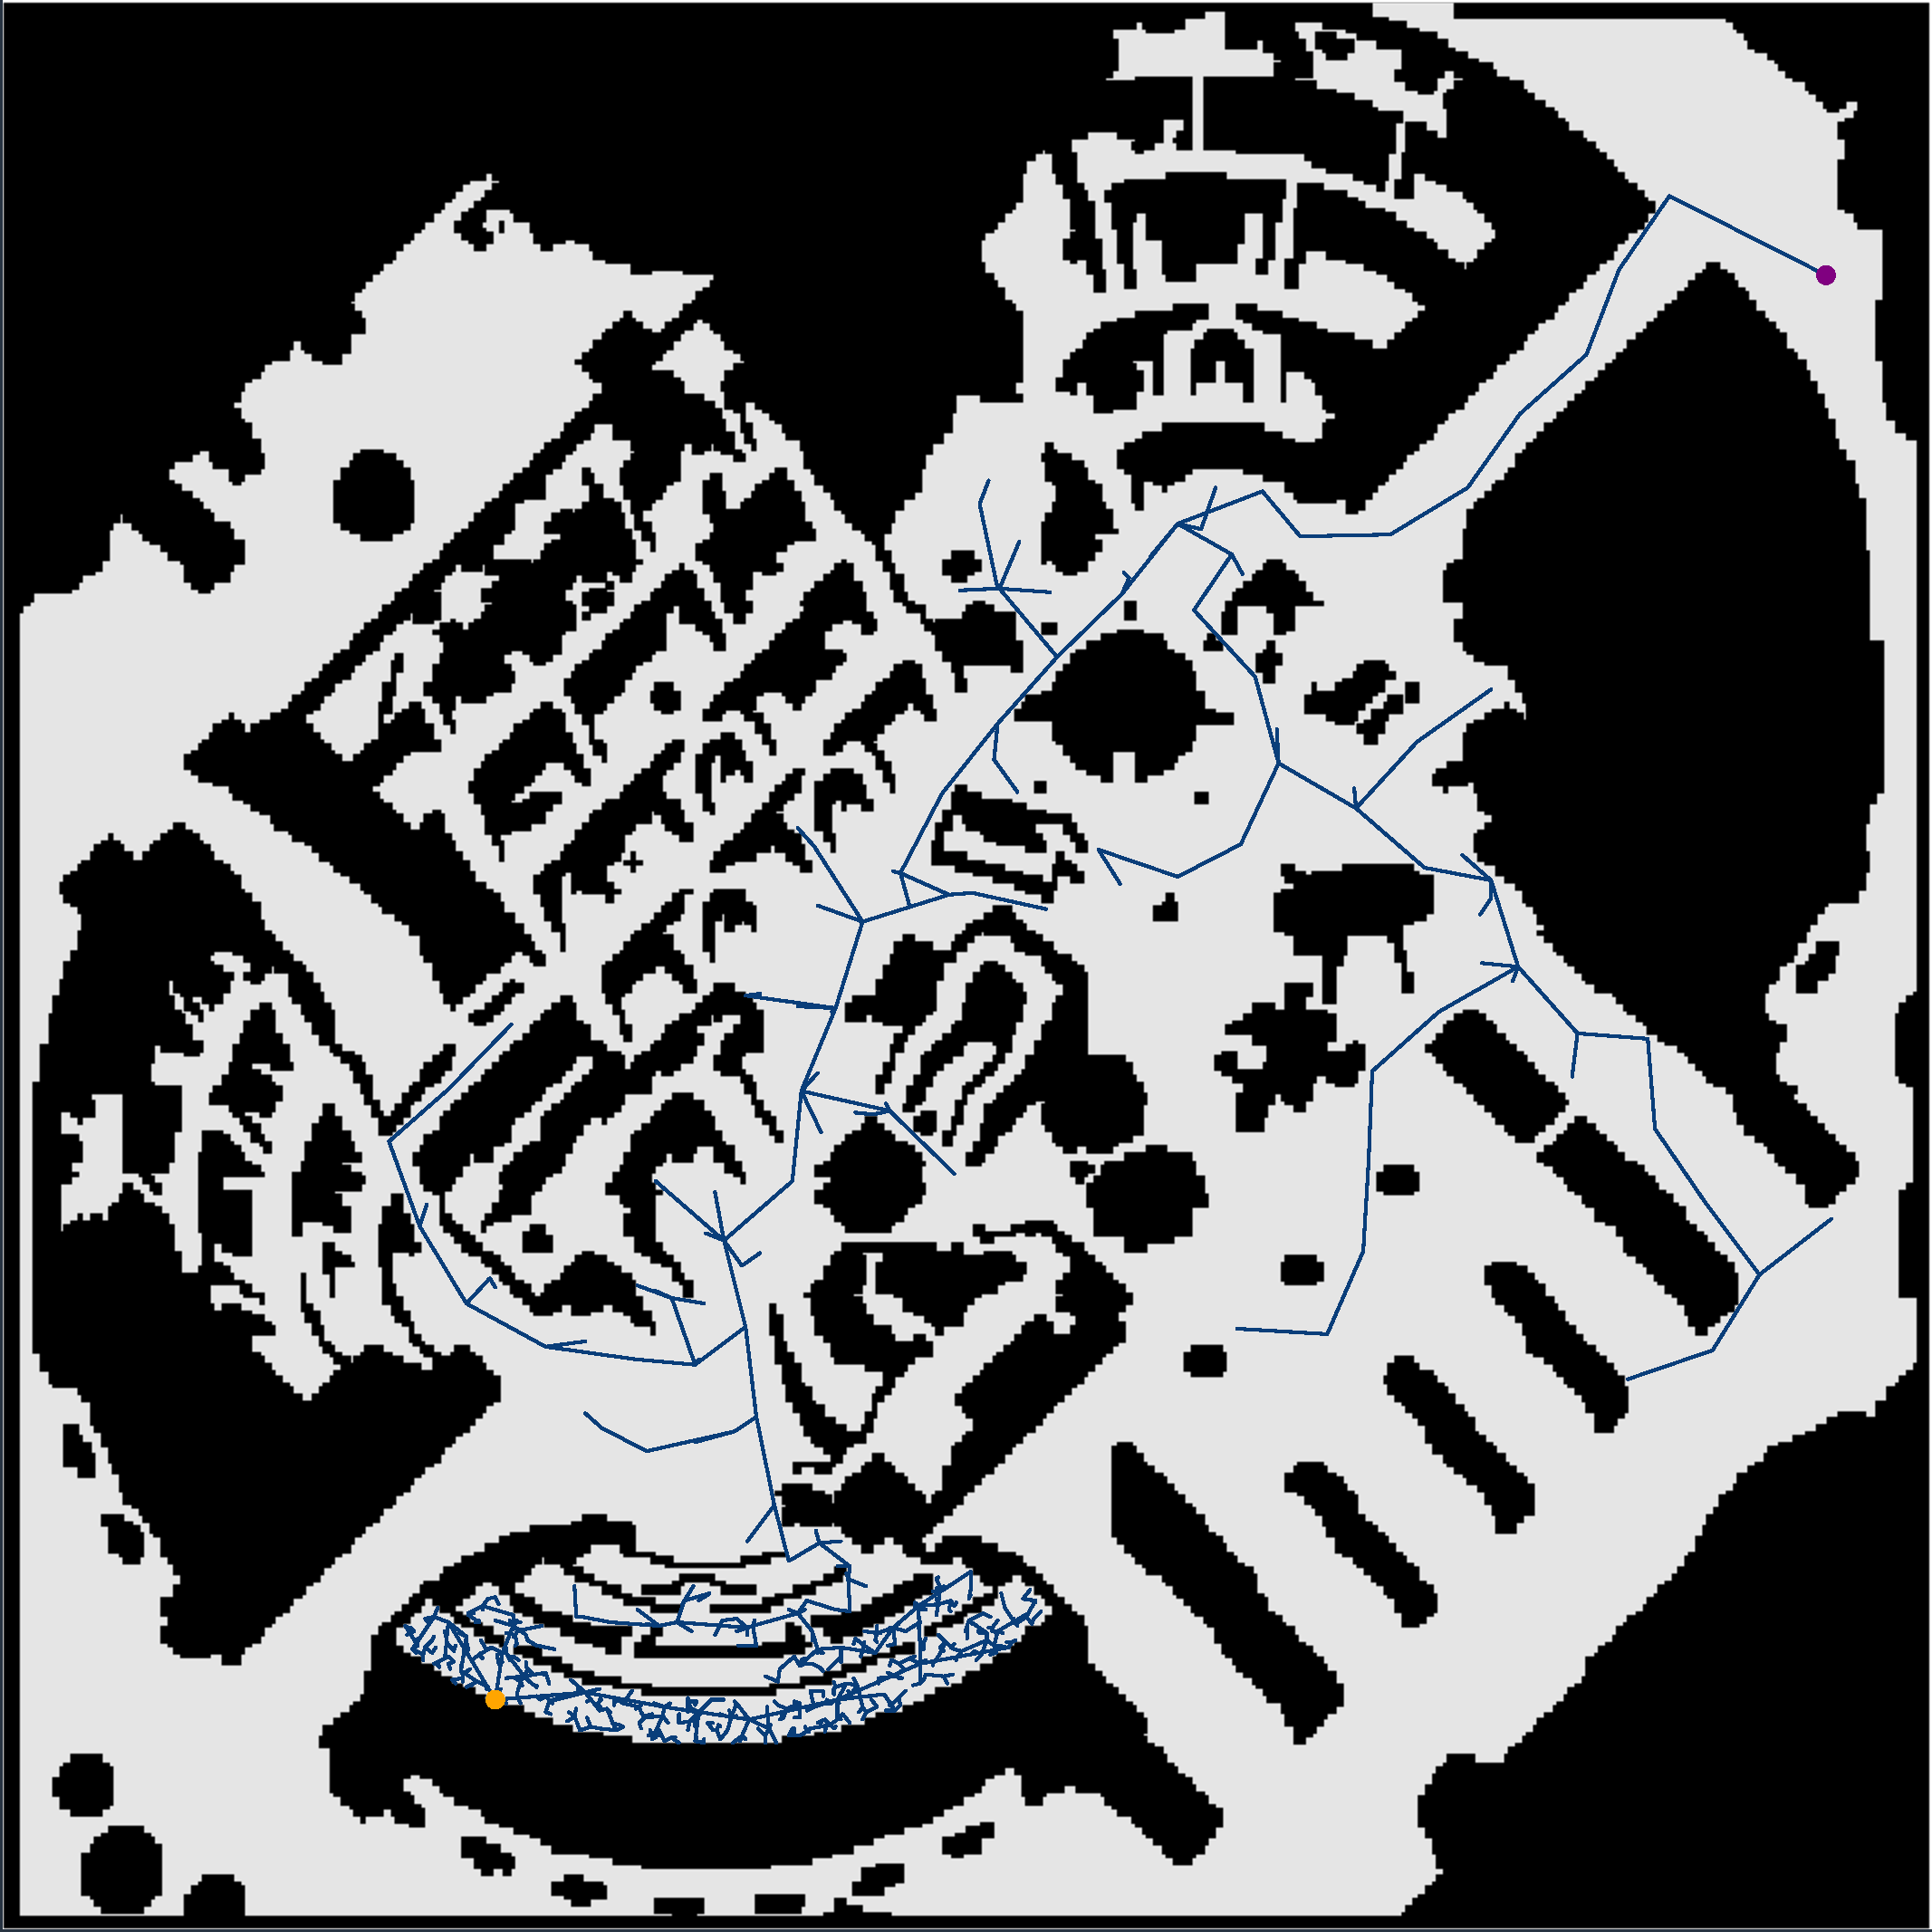
\includegraphics[height=0.7\textheight, keepaspectratio]{figures/baldurs_rrt_one_off.pdf}
      \end{column}
      \begin{column}{.65\linewidth}
          \begin{vfilleditems}
              \item {\Large Rapidly Exploring Random Trees \red{(RRTs)}}
              \begin{itemize}
                  \item RRT*
                  \item Informed RRT*
                  \item Constrained (Multi-phase, RRT-Blossom)
                  \item Dynamic RRT* (RT-RRT*, RRTX, RRT#)
              \end{itemize}
              \vspace{1em}
              \item {\Large Probabilistic Road Maps \red{(PRMs)}}
              \vspace{1em}
              \item {\Large \color{grey} Potential Fields}
          \end{vfilleditems}
      \end{column}
  \end{columns}
\end{frame}

\begin{frame}[plain]{RRT* \white{(Baldur's Gate)}}
    % This figure shows the voronoi regions (in orange)
    %   and convex hull (in pink) of an RRT* run
    % The voronoi regions are the basic operating principle for RRT*
    % Essentially, when a new point is sampled, it will be connected to
    %   its nearest neighbor. Voronoi regions represent which node
    %   is nearest to an *area* of the map.
    % The convex hull shows the total area explored
    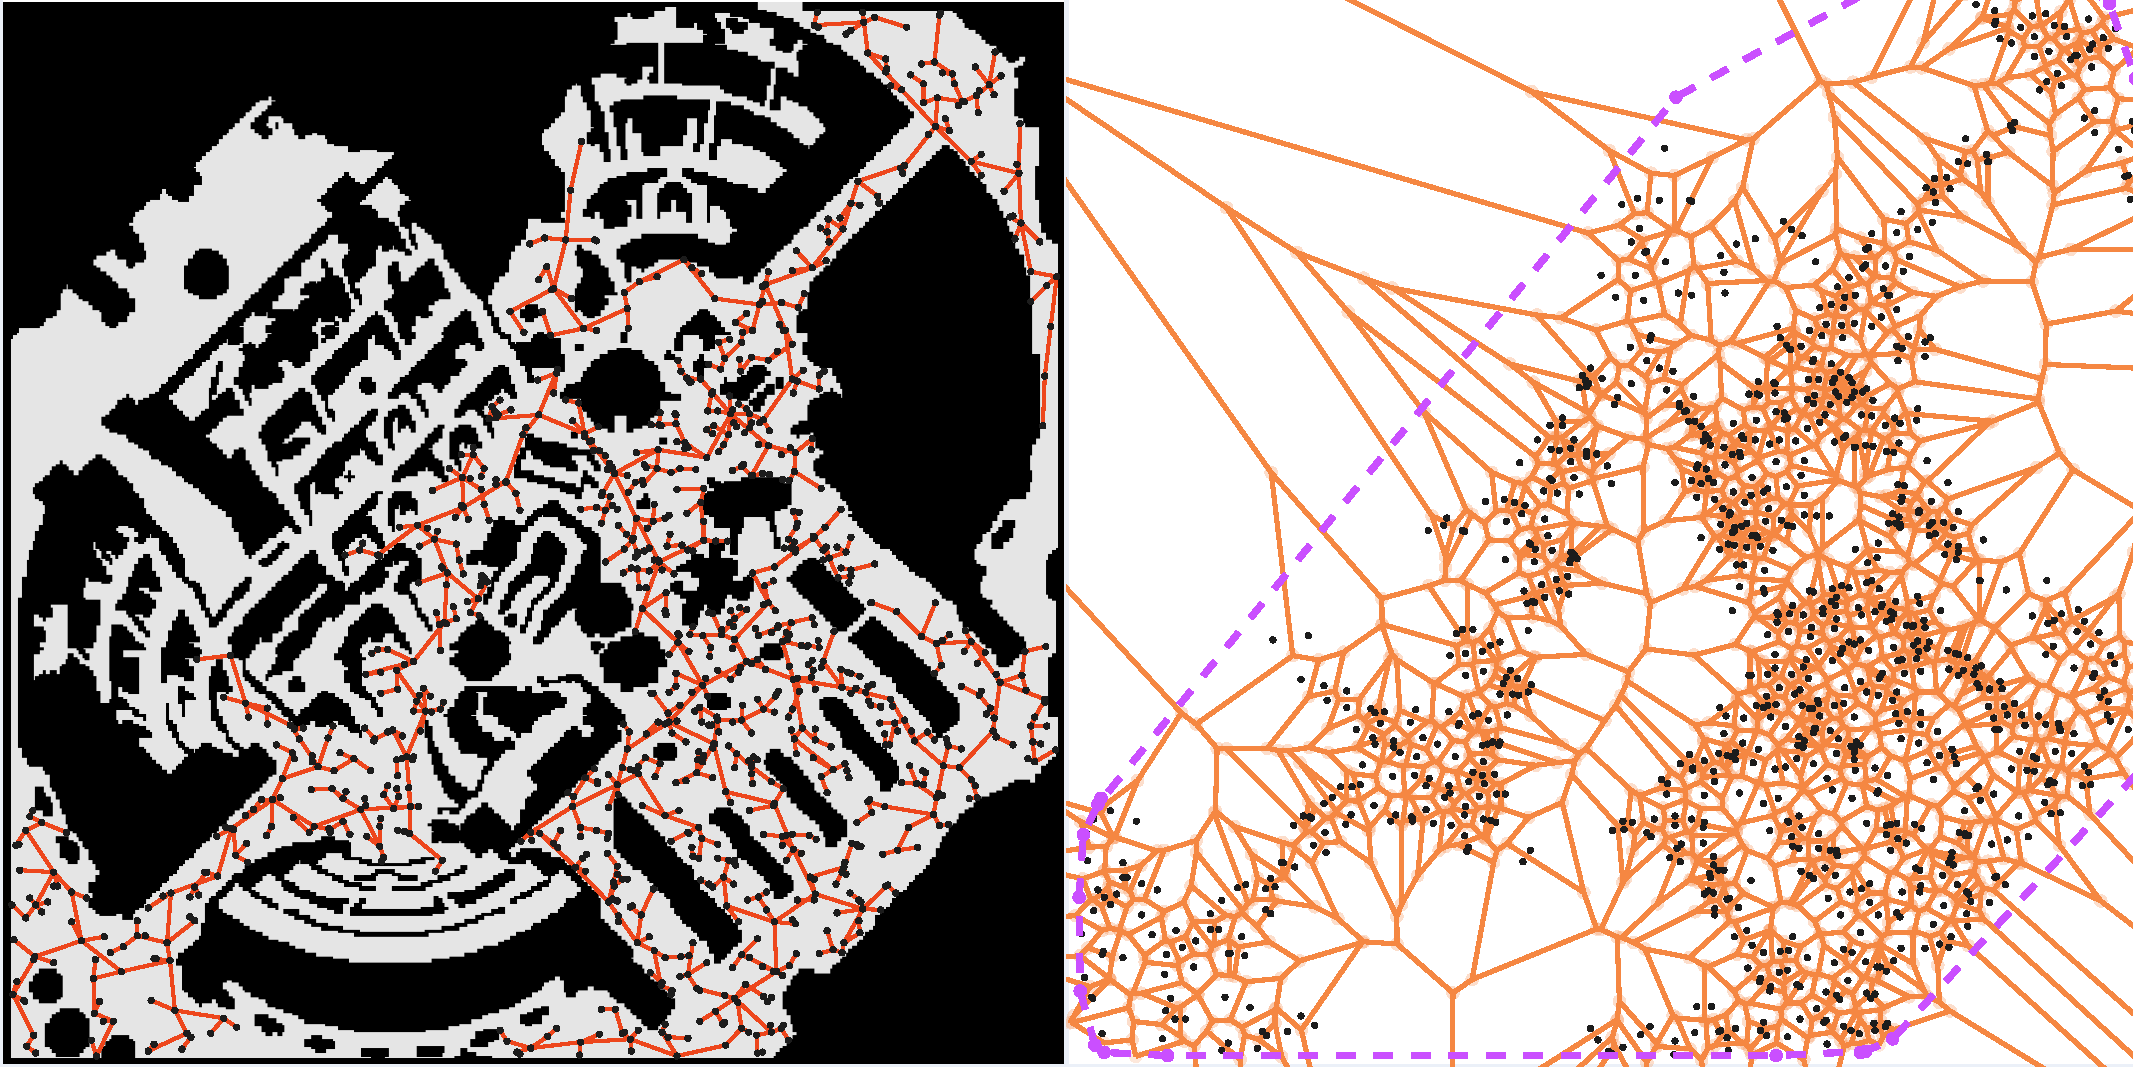
\includegraphics[width=1.0\linewidth, keepaspectratio]{figures/baldurs_1k_explorer.pdf}
\end{frame}

\begin{frame}{Maps Overview {\Medium \color{white}( \cite{sturtevant2012benchmarks})}}
    % Here is an overview of the various 2D maps considered in this thesis
    % This includes maps from video games, such as:
    %   - Baldur's Gate
    %   - Dragon Age
    %   - Starcraft
    %   - World of Warcraft
    % However, it also includes obstacle maps of large cities, such as:
    %   - Boston, Shanghai, Milan
    % Finally, it includes several mazes, and even some Amazon warehouses
    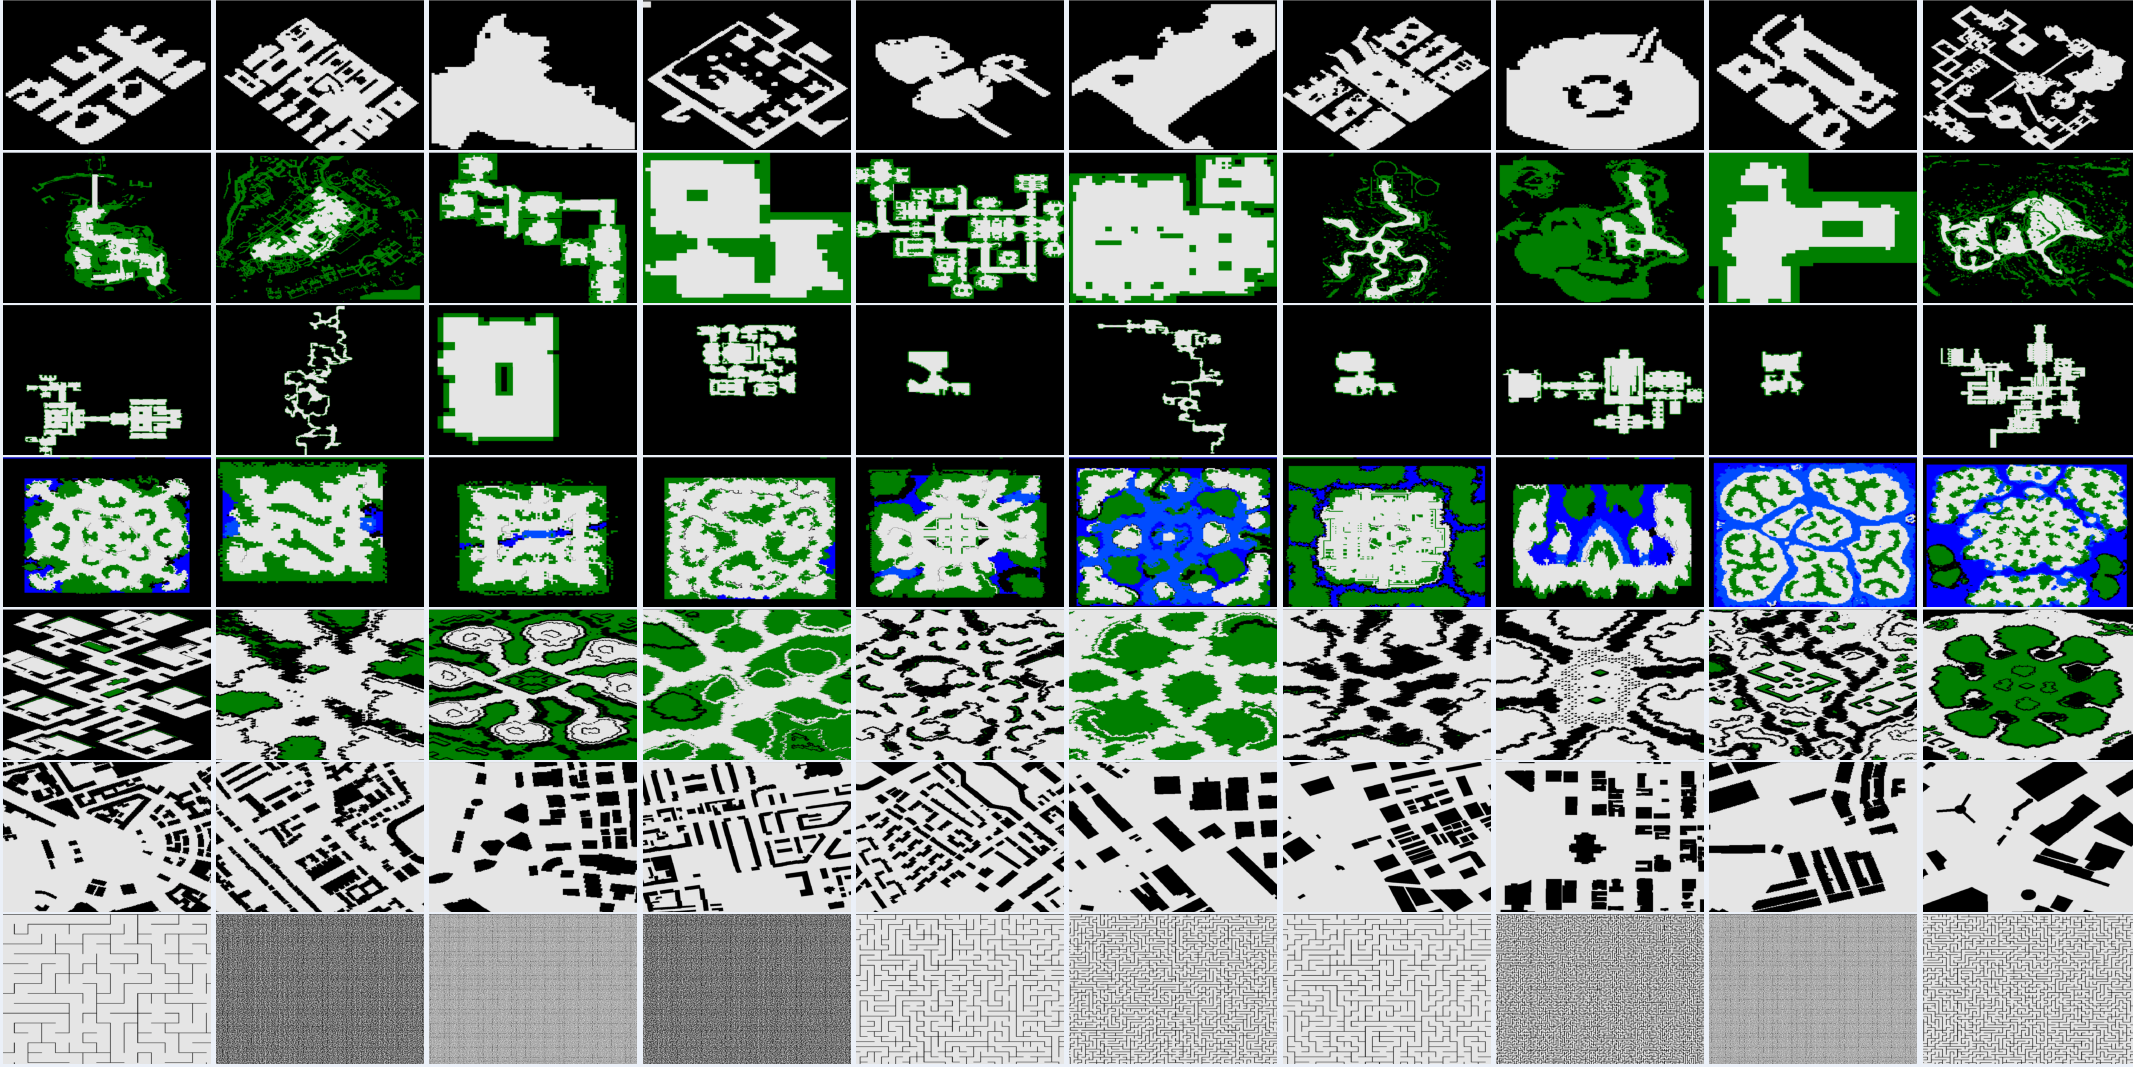
\includegraphics[width=0.95\linewidth, keepaspectratio]{figures/show_maps_overview.pdf}
\end{frame}

\begin{frame}{Maps Detail {\Medium \color{white}( \cite{sturtevant2012benchmarks})}}
    % Here, we see various maps in closer detail.
    % Many maps in this dataset have unique characteristics.
    % For example, this Shanghai map, or the bottom-left Dragon Age map are both relatively open.
    % In contrast, the Boston map and Starcraft: Frozen Sea map are cluttered.
    % The Baldur's gate map, the maze, and the Dragon Age mansion map all have narrow corridors.
    % Because each map has it's own characteristics, the goal of this thesis is to specialize algorithms to each of them.
    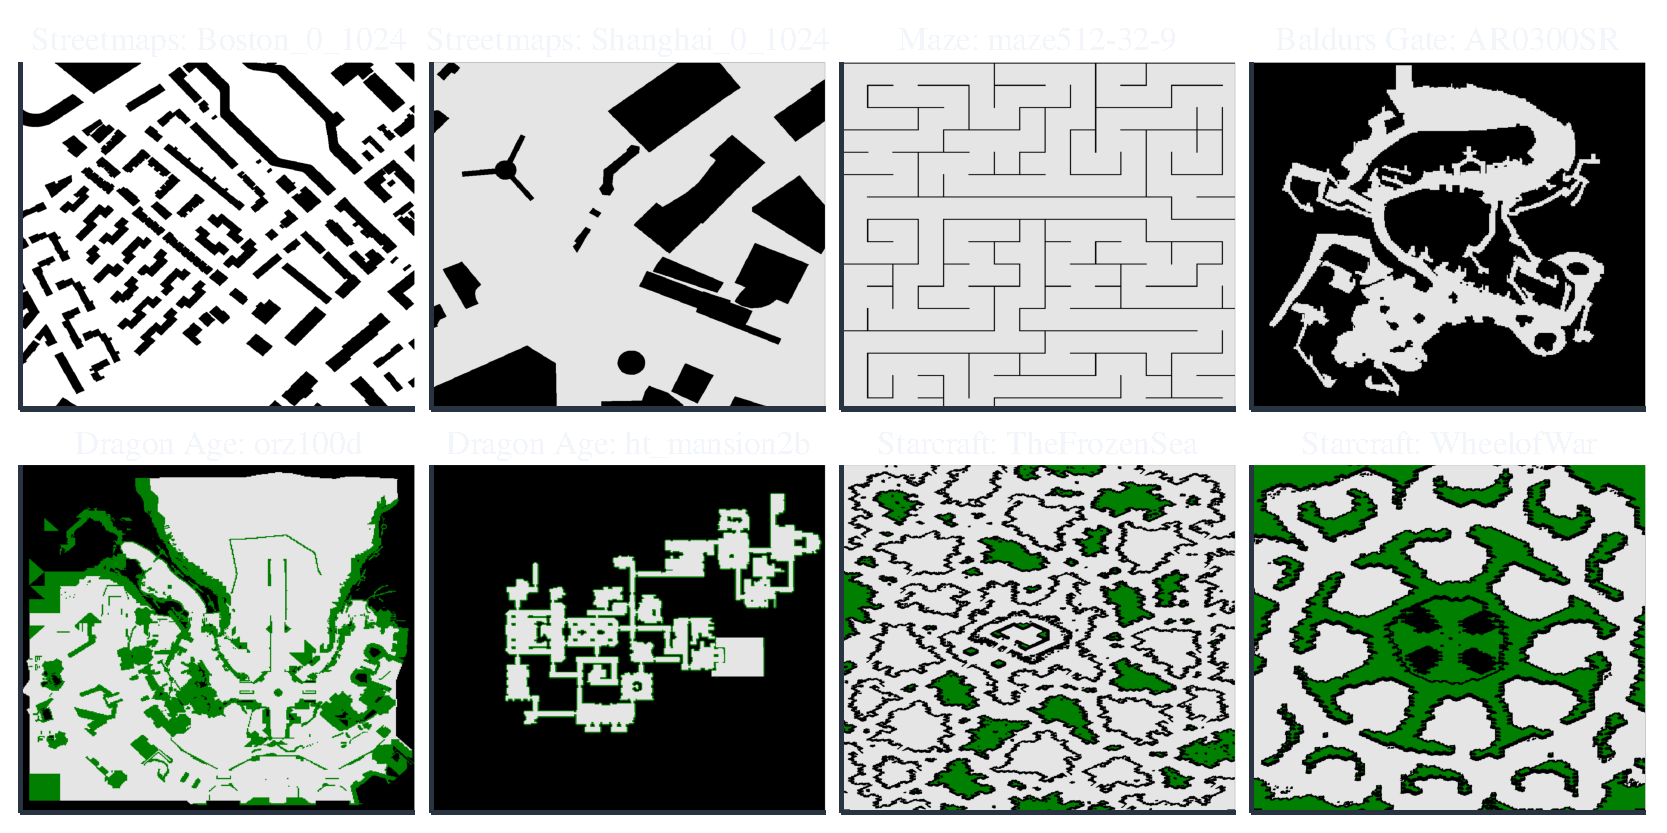
\includegraphics[width=1.0\linewidth, keepaspectratio]{figures/show_maps.pdf}
\end{frame}

\begin{frame}{Specialization Results}
  \begin{columns}[T]
      \begin{column}{.6\linewidth}
      \centering
      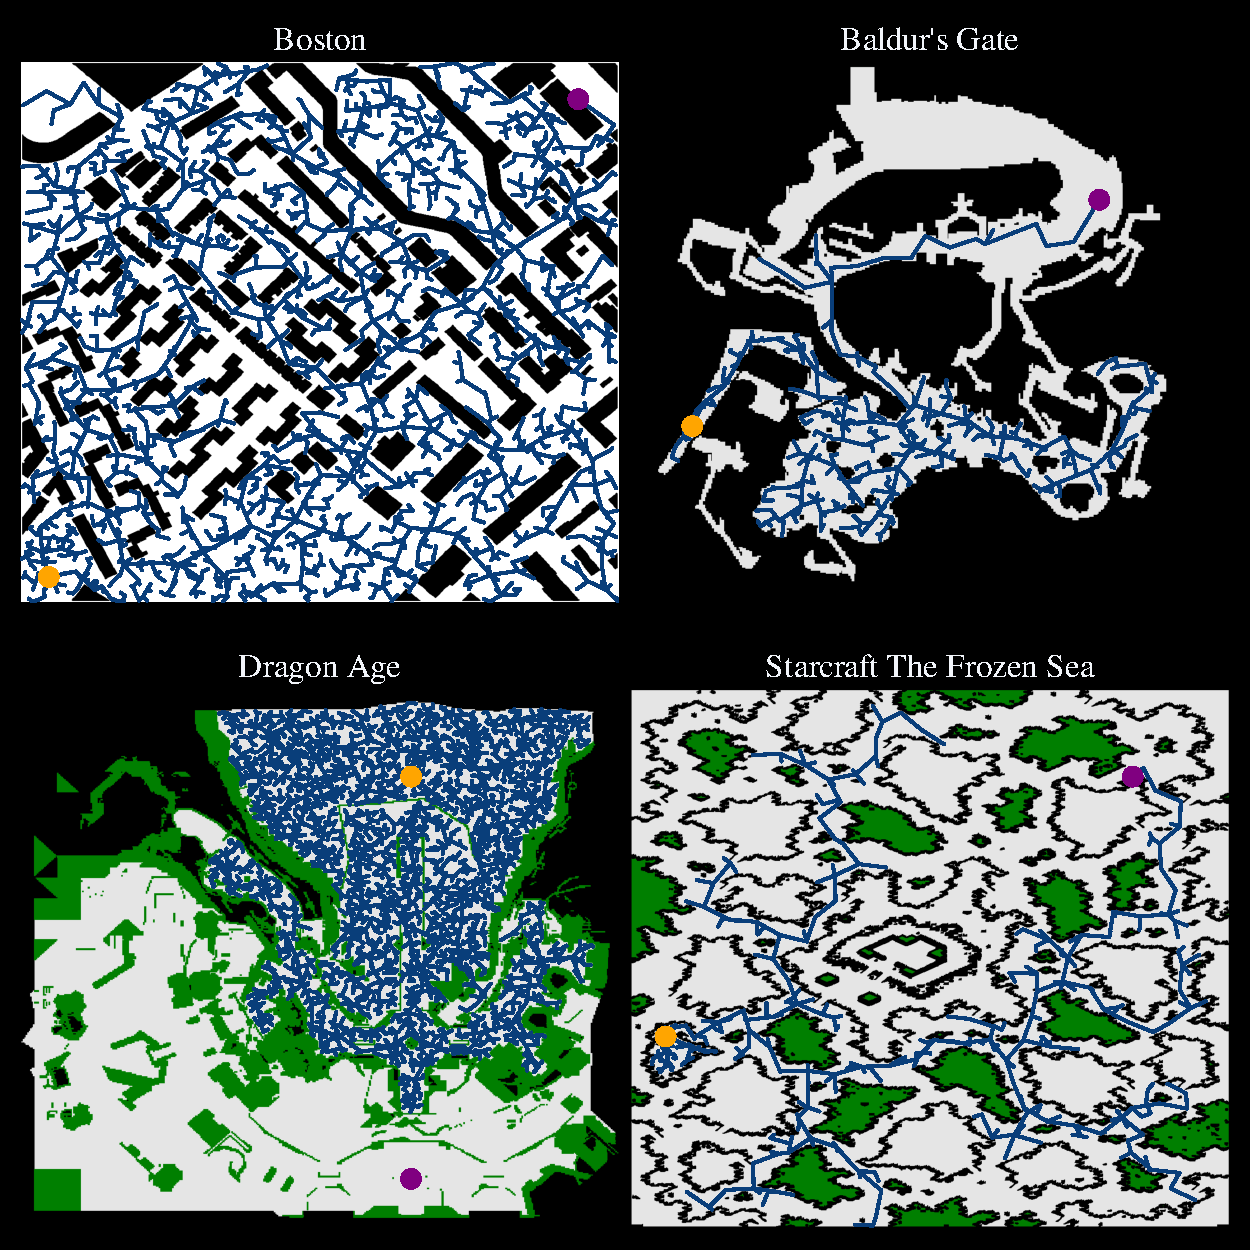
\includegraphics[height=0.83\textheight]{figures/learned2.pdf}
      \end{column}
      \begin{column}{.4\linewidth}
      \epigraph{
      There is no “silver bullet” algorithm for solving all path planning problems. Heuristics that lead to massive speed-up in one scenario might be detrimental in others. Also, algorithmic parameters are mostly ad-hoc and correctly tuning them to a specific environment might drastically increase performance.
      }{\textit{
      Nikolaus Correll
      }}
      \end{column}
  \end{columns}
\end{frame}

\begin{frame}{Specialization Results}
    % Here are the results of specializing algorithms to particular maps.
    % This experiment looked at five different scenarios:
    %   Milan, Italy, (in the top left) which is a relatively cluttered map
    %   A blank map   (in the bottom right) which is intentionally open and easy to specialize to.
    %   Three starcraft maps: Enigma, Turbo, and Entanglement.
    %   Milan and the blank map are meant to be controls,
    %     while the starcraft maps are the main experiment.
    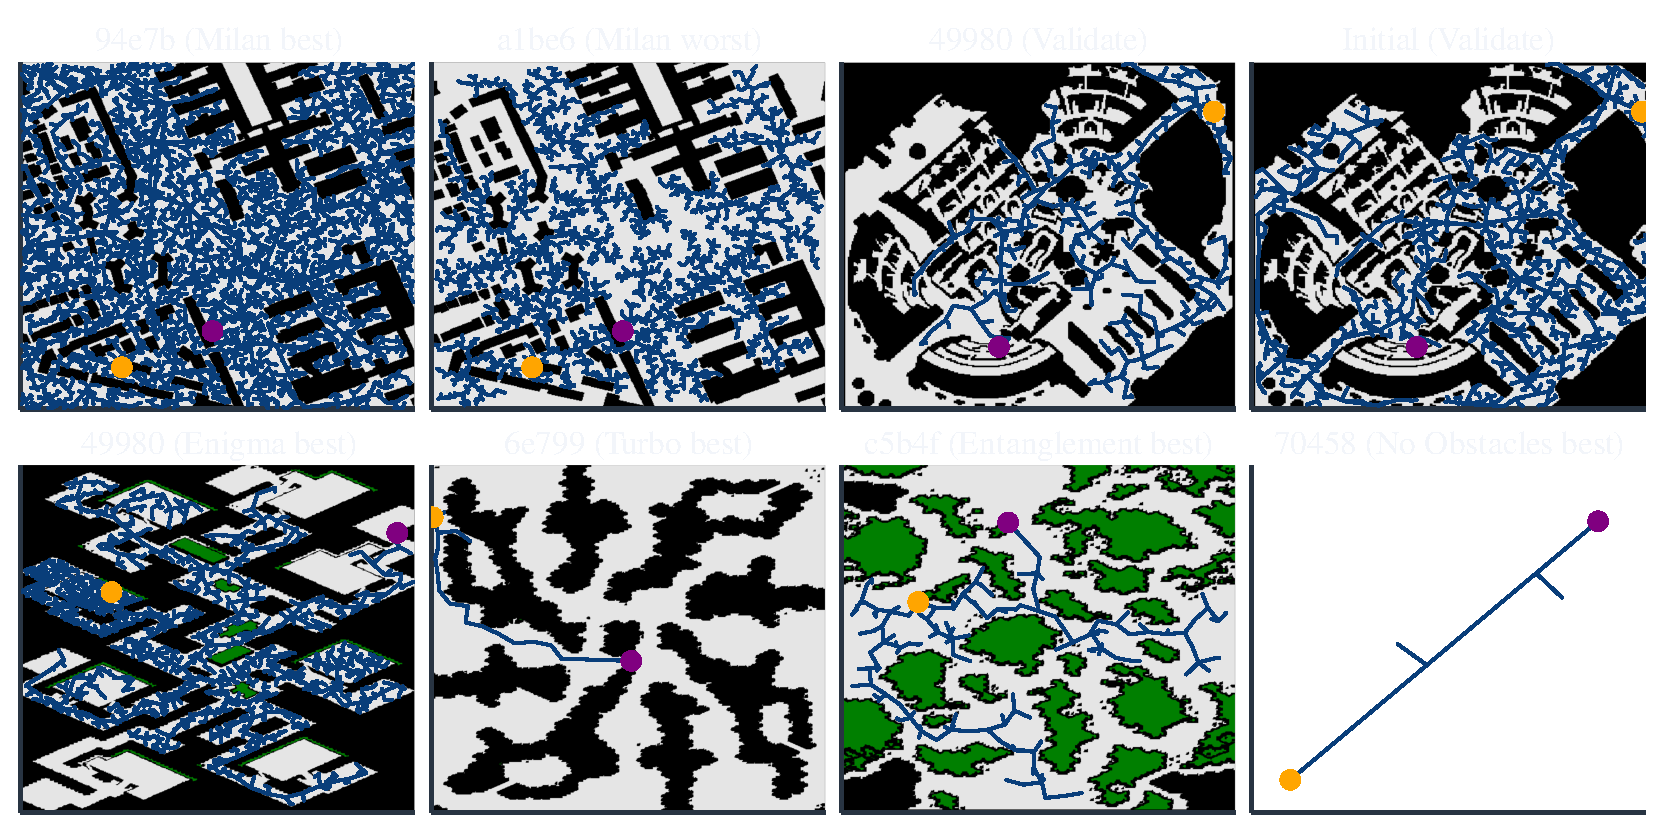
\includegraphics[width=1.0\linewidth, keepaspectratio]{figures/learned.pdf}
\end{frame}

\begin{frame}[plain, noframenumbering]
  \centering
  \vfill
  {\fontsize{40}{50}\selectfont \red{Methods}}
  \vfill
\end{frame}

\begin{frame}{AutoML-Zero: Evolving Machine Learning Algorithms From Scratch \white{\cite{real2020automl}}}
    \begin{vfilleditems}
        \item \Huge Learns ML practices on CIFAR-10 
        \vspace{0.7em}
        \item \Huge Tensor register machine
        \vspace{0.7em}
        \item \emph{Regularized Evolution} 
    \end{vfilleditems}
\end{frame}

\begin{frame}[plain]{AutoML-Zero \white{\cite{real2020automl}}}
\begin{figure}
\centering
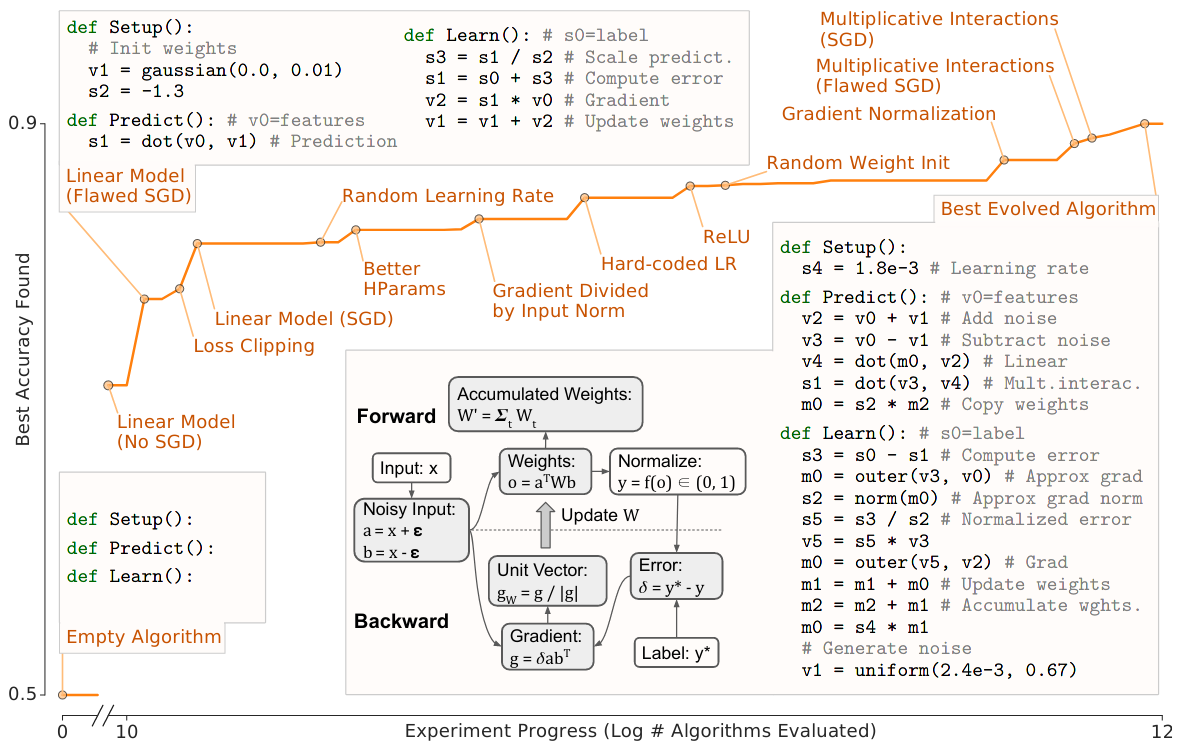
\includegraphics[scale=0.37]{figures/automl_zero_main_fig.png}
\end{figure}
\end{frame}

\begin{frame}{\white{Algorithm Choice:}}

  \begin{columns}[T]
      \begin{column}{.6\linewidth}
        \begin{vfilleditems}
            \item \emph{Pareto Evolution}
            \begin{itemize}
                \item Multi-objective
            \end{itemize}
            \vspace{1em}
            $O(g * m * n^2)$
        \end{vfilleditems}
      \end{column}
      \begin{column}{.7\linewidth}
        \begin{vfilleditems}
            \item \emph{Regularized Evolution}
            \begin{itemize}
                \item Single-objective
            \end{itemize}
            \vspace{1em}
            $O(g * p)$
        \end{vfilleditems}
      \end{column}
  \end{columns}
  \begin{center}
  {\Large Where \color{m1} $g = $ generations}
  \newline
  {\Large \hspace{6em} \color{m1} $m = $ objectives}
  \newline
  {\Large \hspace{6em} $n = $ total population size}
  \newline
  {\Large \hspace{6em} $p = $ sample size}
  \end{center}
\end{frame}

\begin{frame}{{\color{pureminimalistic@text@white} Multiple Objectives}}
  \begin{columns}[T]
      \begin{column}{.4\linewidth}
          \begin{vfilleditems}
              \item \emph{Nodes}
              \vspace{1em}
              \item \emph{Path Length}
              \vspace{1em}
              \item {\Large Often, these objectives compete}
          \end{vfilleditems}
      \end{column}
      \begin{column}{.6\linewidth}
      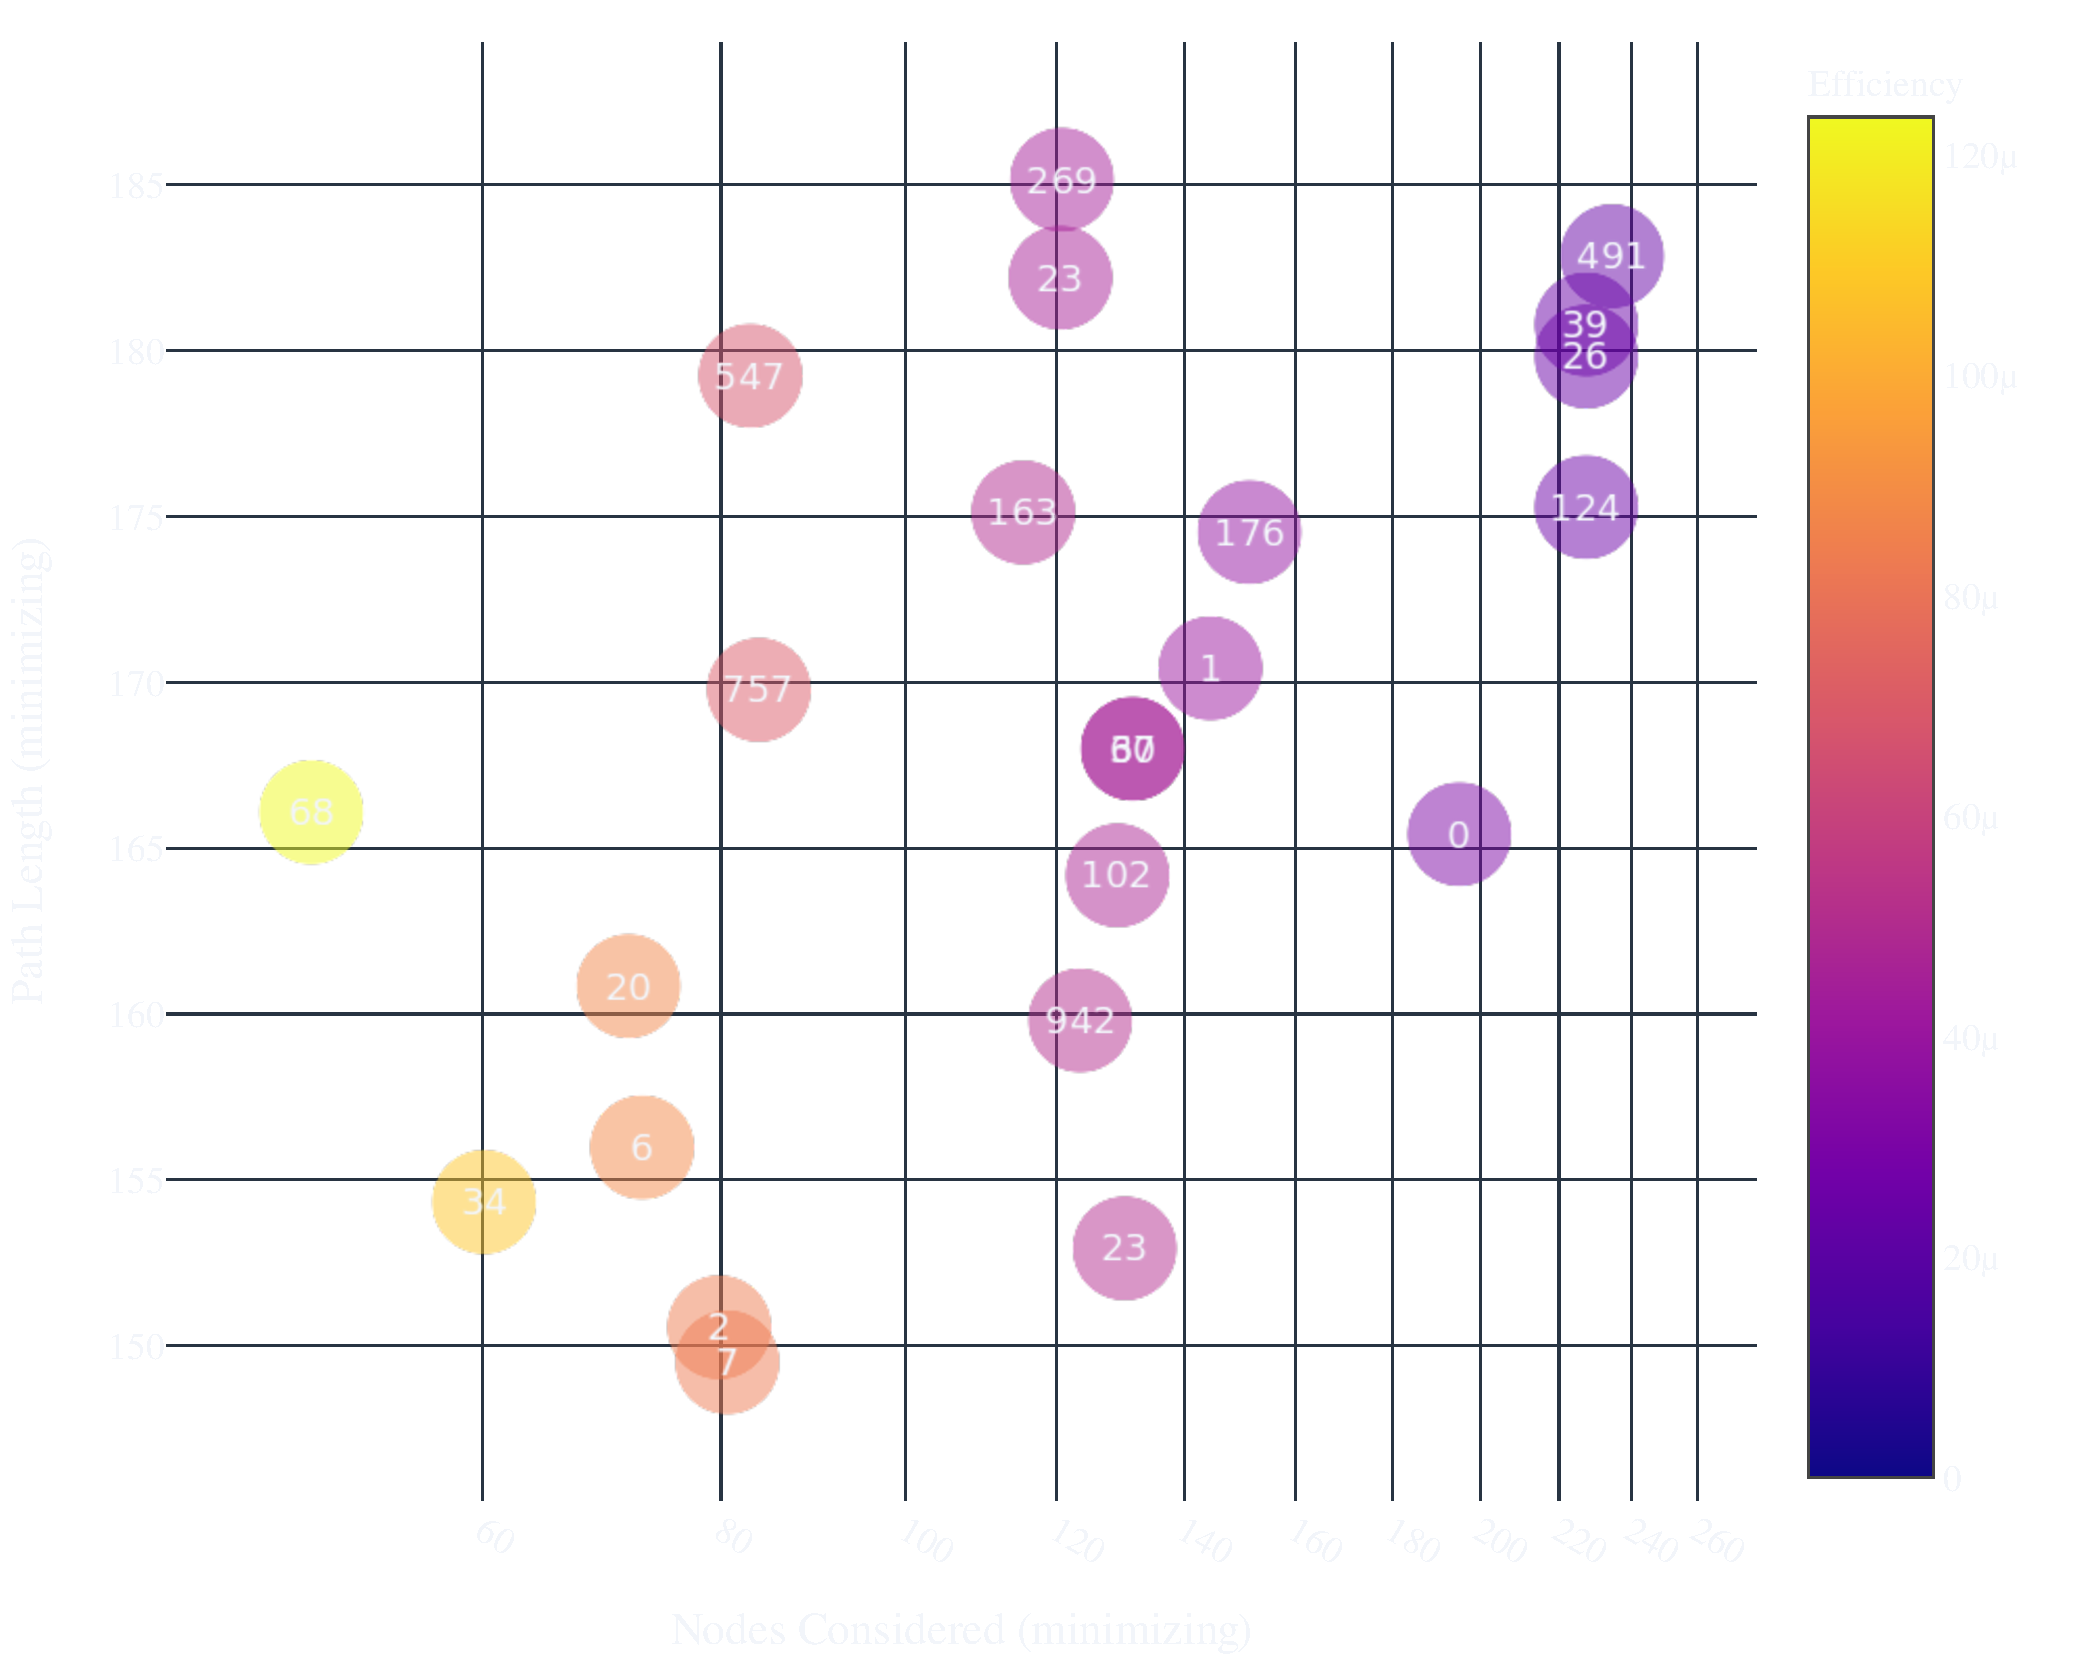
\includegraphics[width=0.9\linewidth, keepaspectratio]{figures/total_overview.pdf}
      \end{column}
  \end{columns}
\end{frame}

\begin{frame}{{Pareto Fronts}}
  \begin{columns}[T]
      \begin{column}{.4\linewidth}
          \begin{vfilleditems}
              \item {\Large Vectorized Fitness}
              \vspace{1em}
              \newline {\Large $v$ = $\{60, 155\}$}
          \end{vfilleditems}
      \end{column}
      \begin{column}{.6\linewidth}
      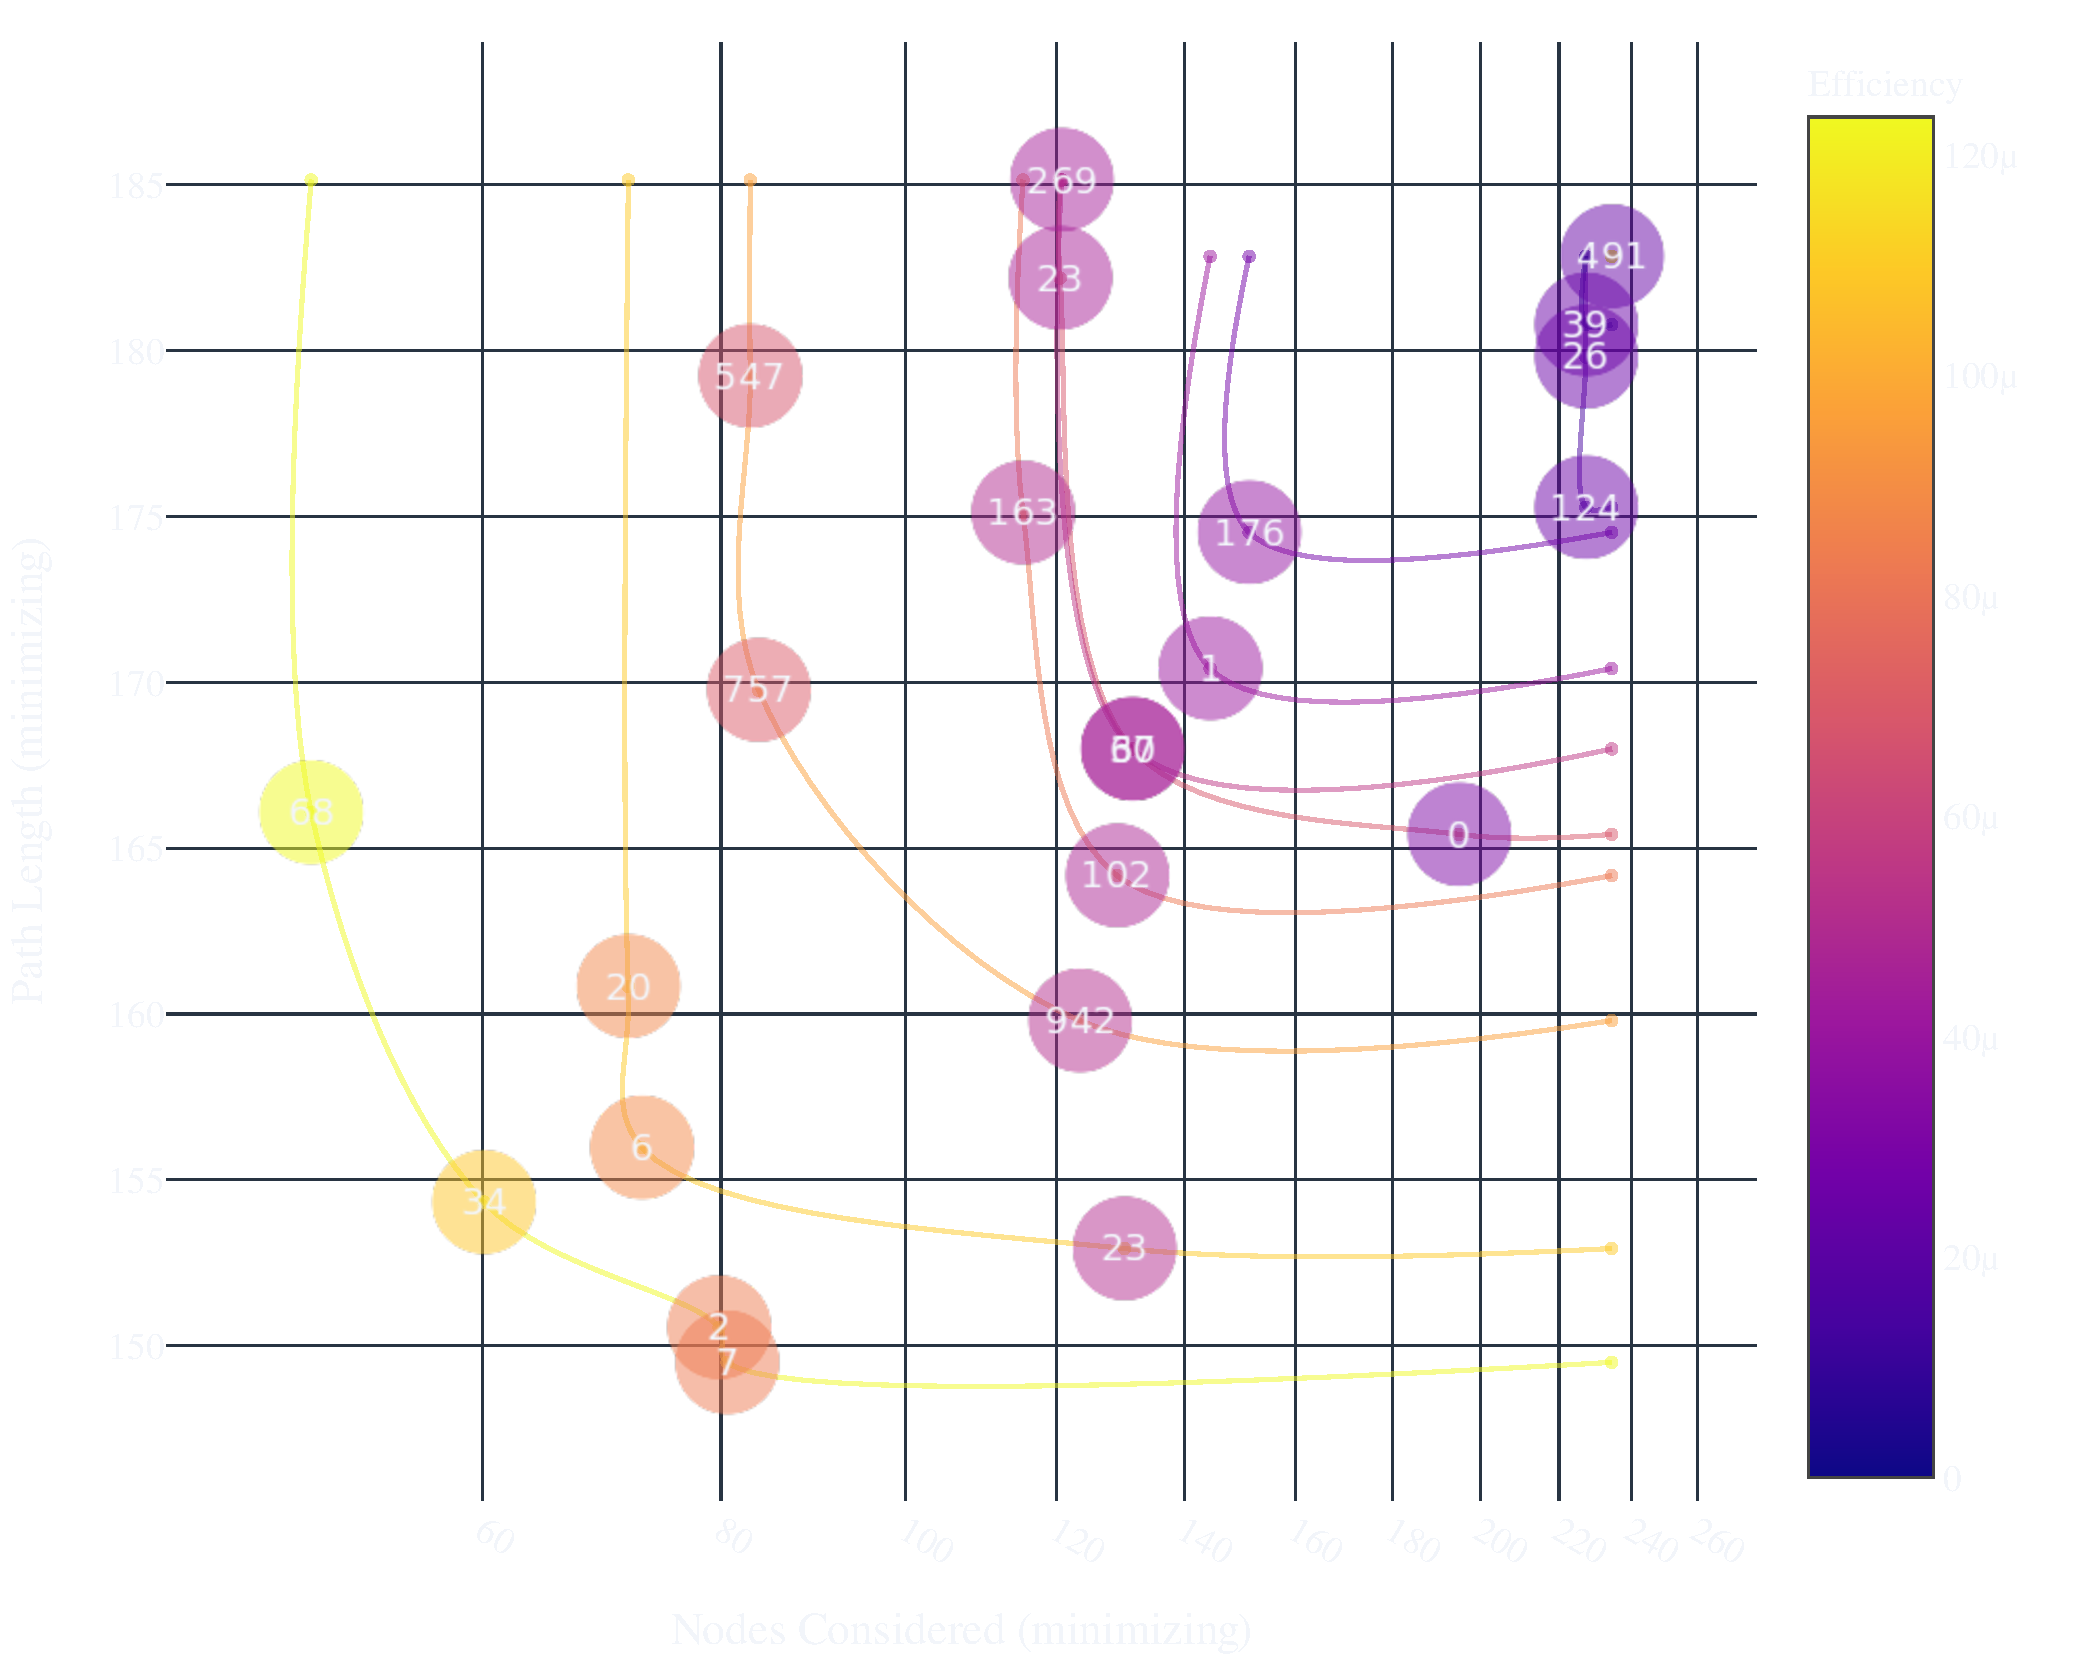
\includegraphics[width=0.9\linewidth, keepaspectratio]{figures/total_pareto_overview.pdf}
      \end{column}
  \end{columns}
\end{frame}


\begin{frame}{Pareto Evolution}
    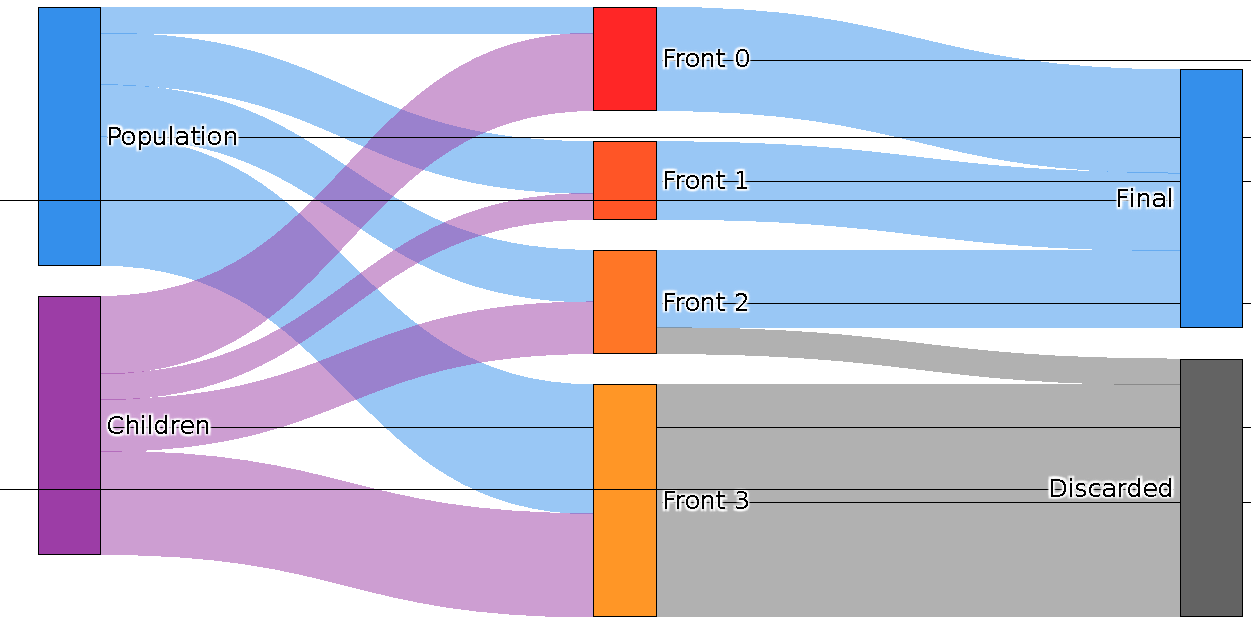
\includegraphics[width=1.0\linewidth, keepaspectratio]{figures/paretoev.pdf}
\end{frame}

\begin{frame}{Population Dynamics: Starcraft Engima}
    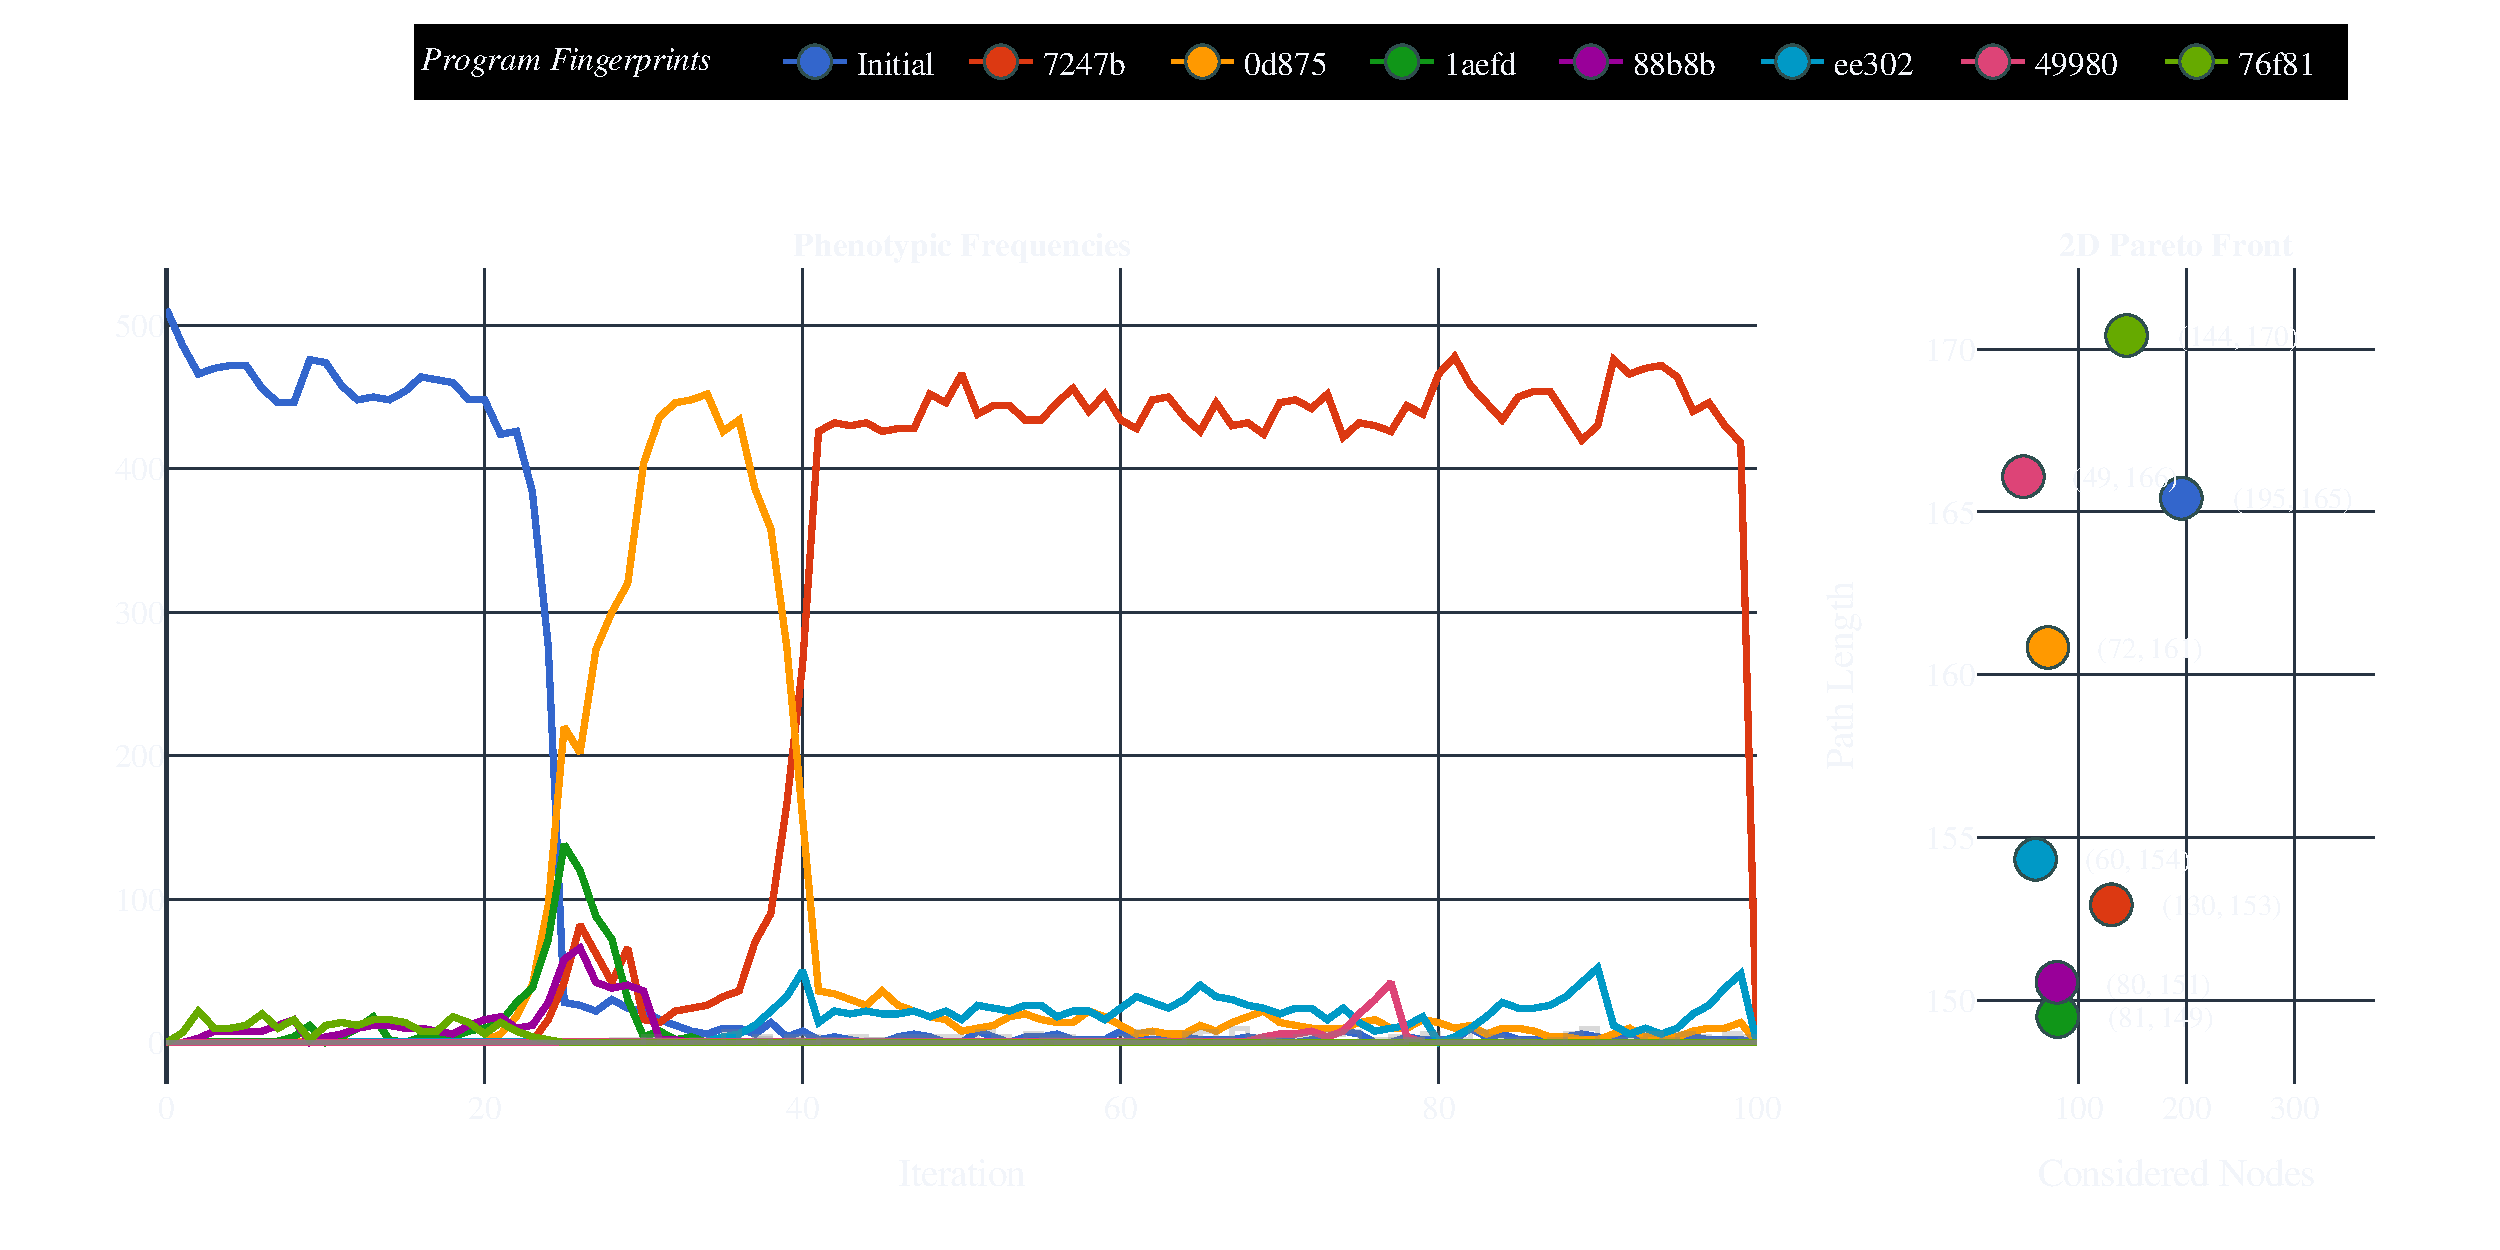
\includegraphics[width=1.0\linewidth, keepaspectratio]{figures/early_pheno.pdf}
\end{frame}

\begin{frame}{Population Dynamics: Starcraft Engima}
    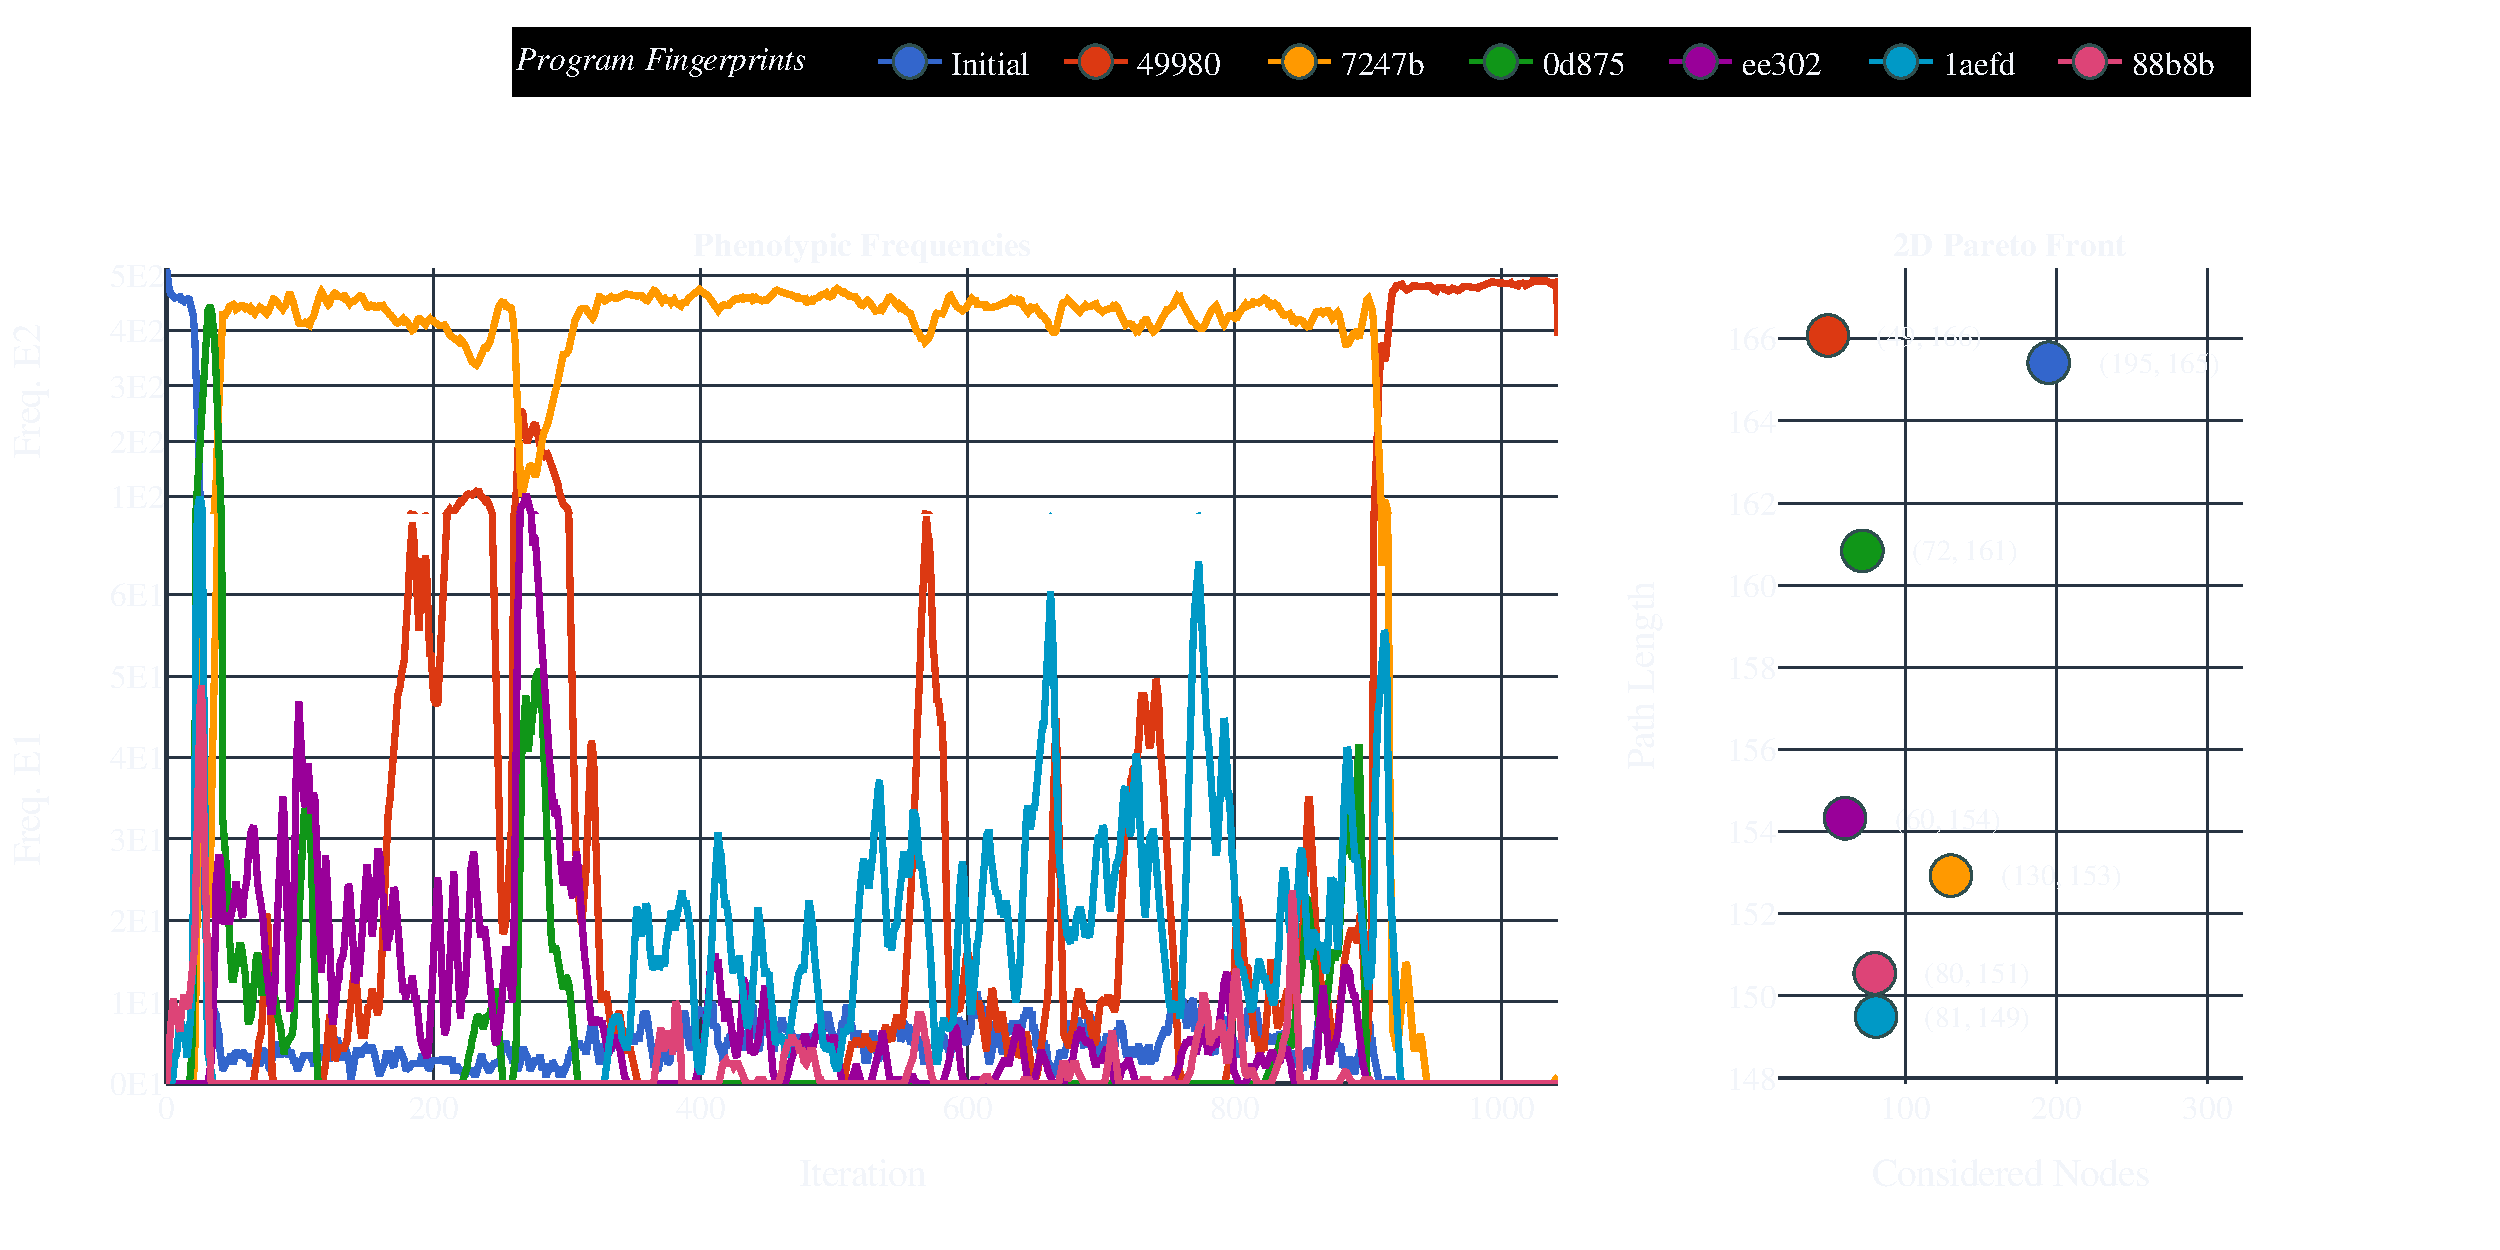
\includegraphics[width=1.0\linewidth, keepaspectratio]{figures/pheno.pdf}
\end{frame}

\begin{frame}{Population Dynamics: Baldur's Gate}
    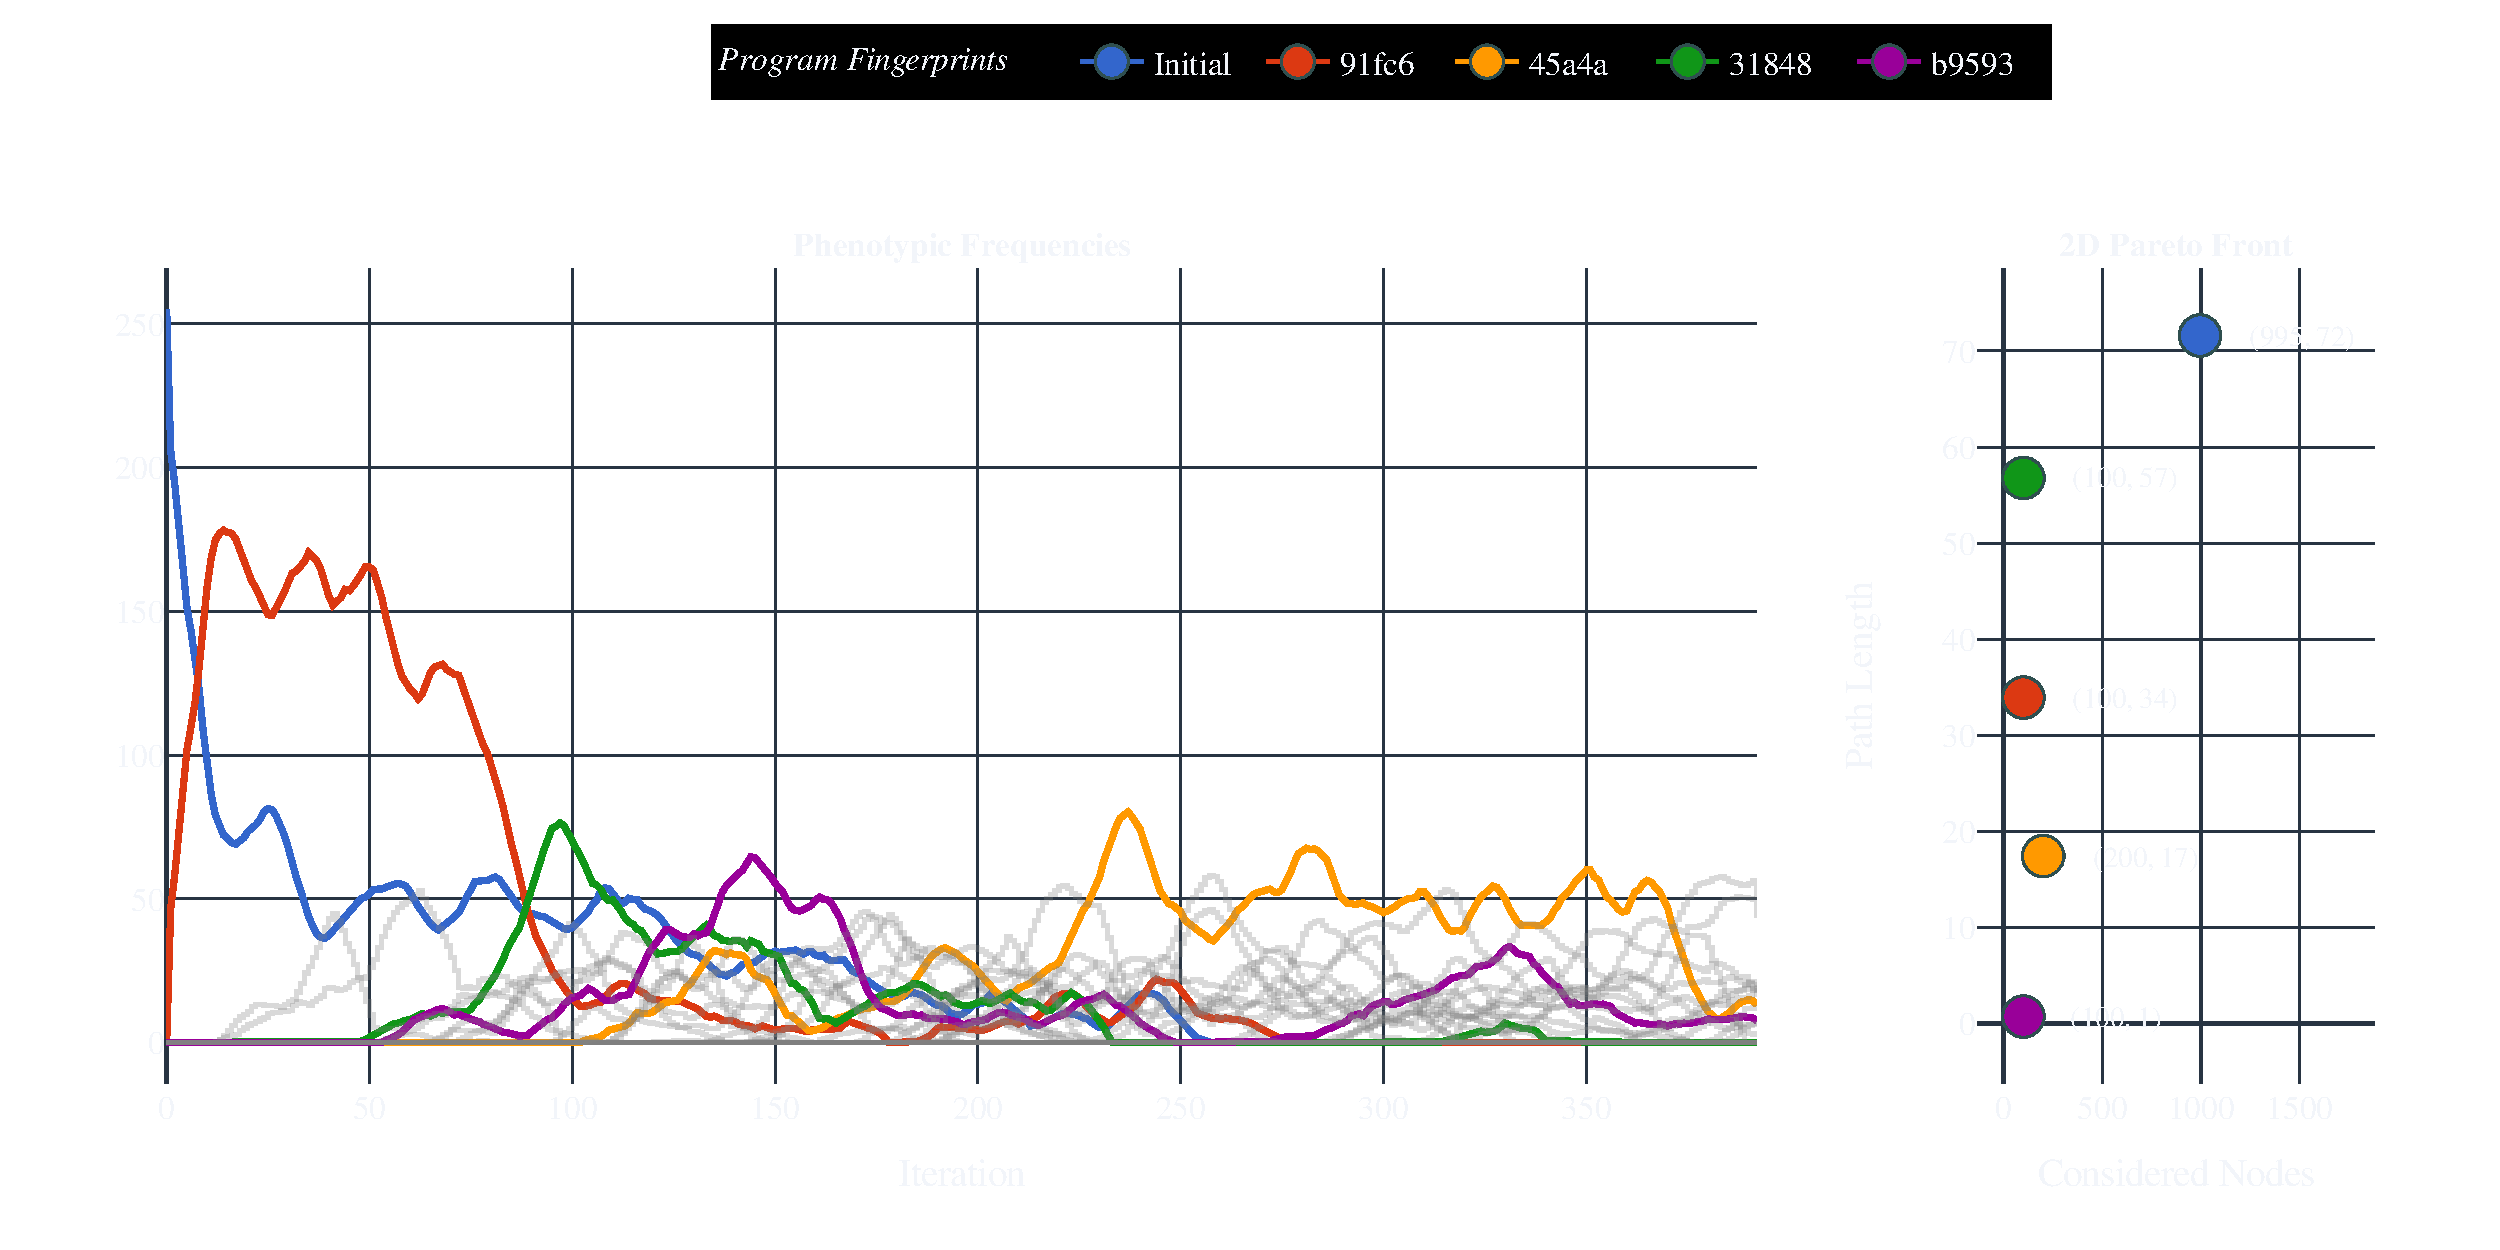
\includegraphics[width=1.0\linewidth, keepaspectratio]{figures/baldurs_pheno_60.pdf}
\end{frame}

\begin{frame}{Efficient Exploration}
    \centering
    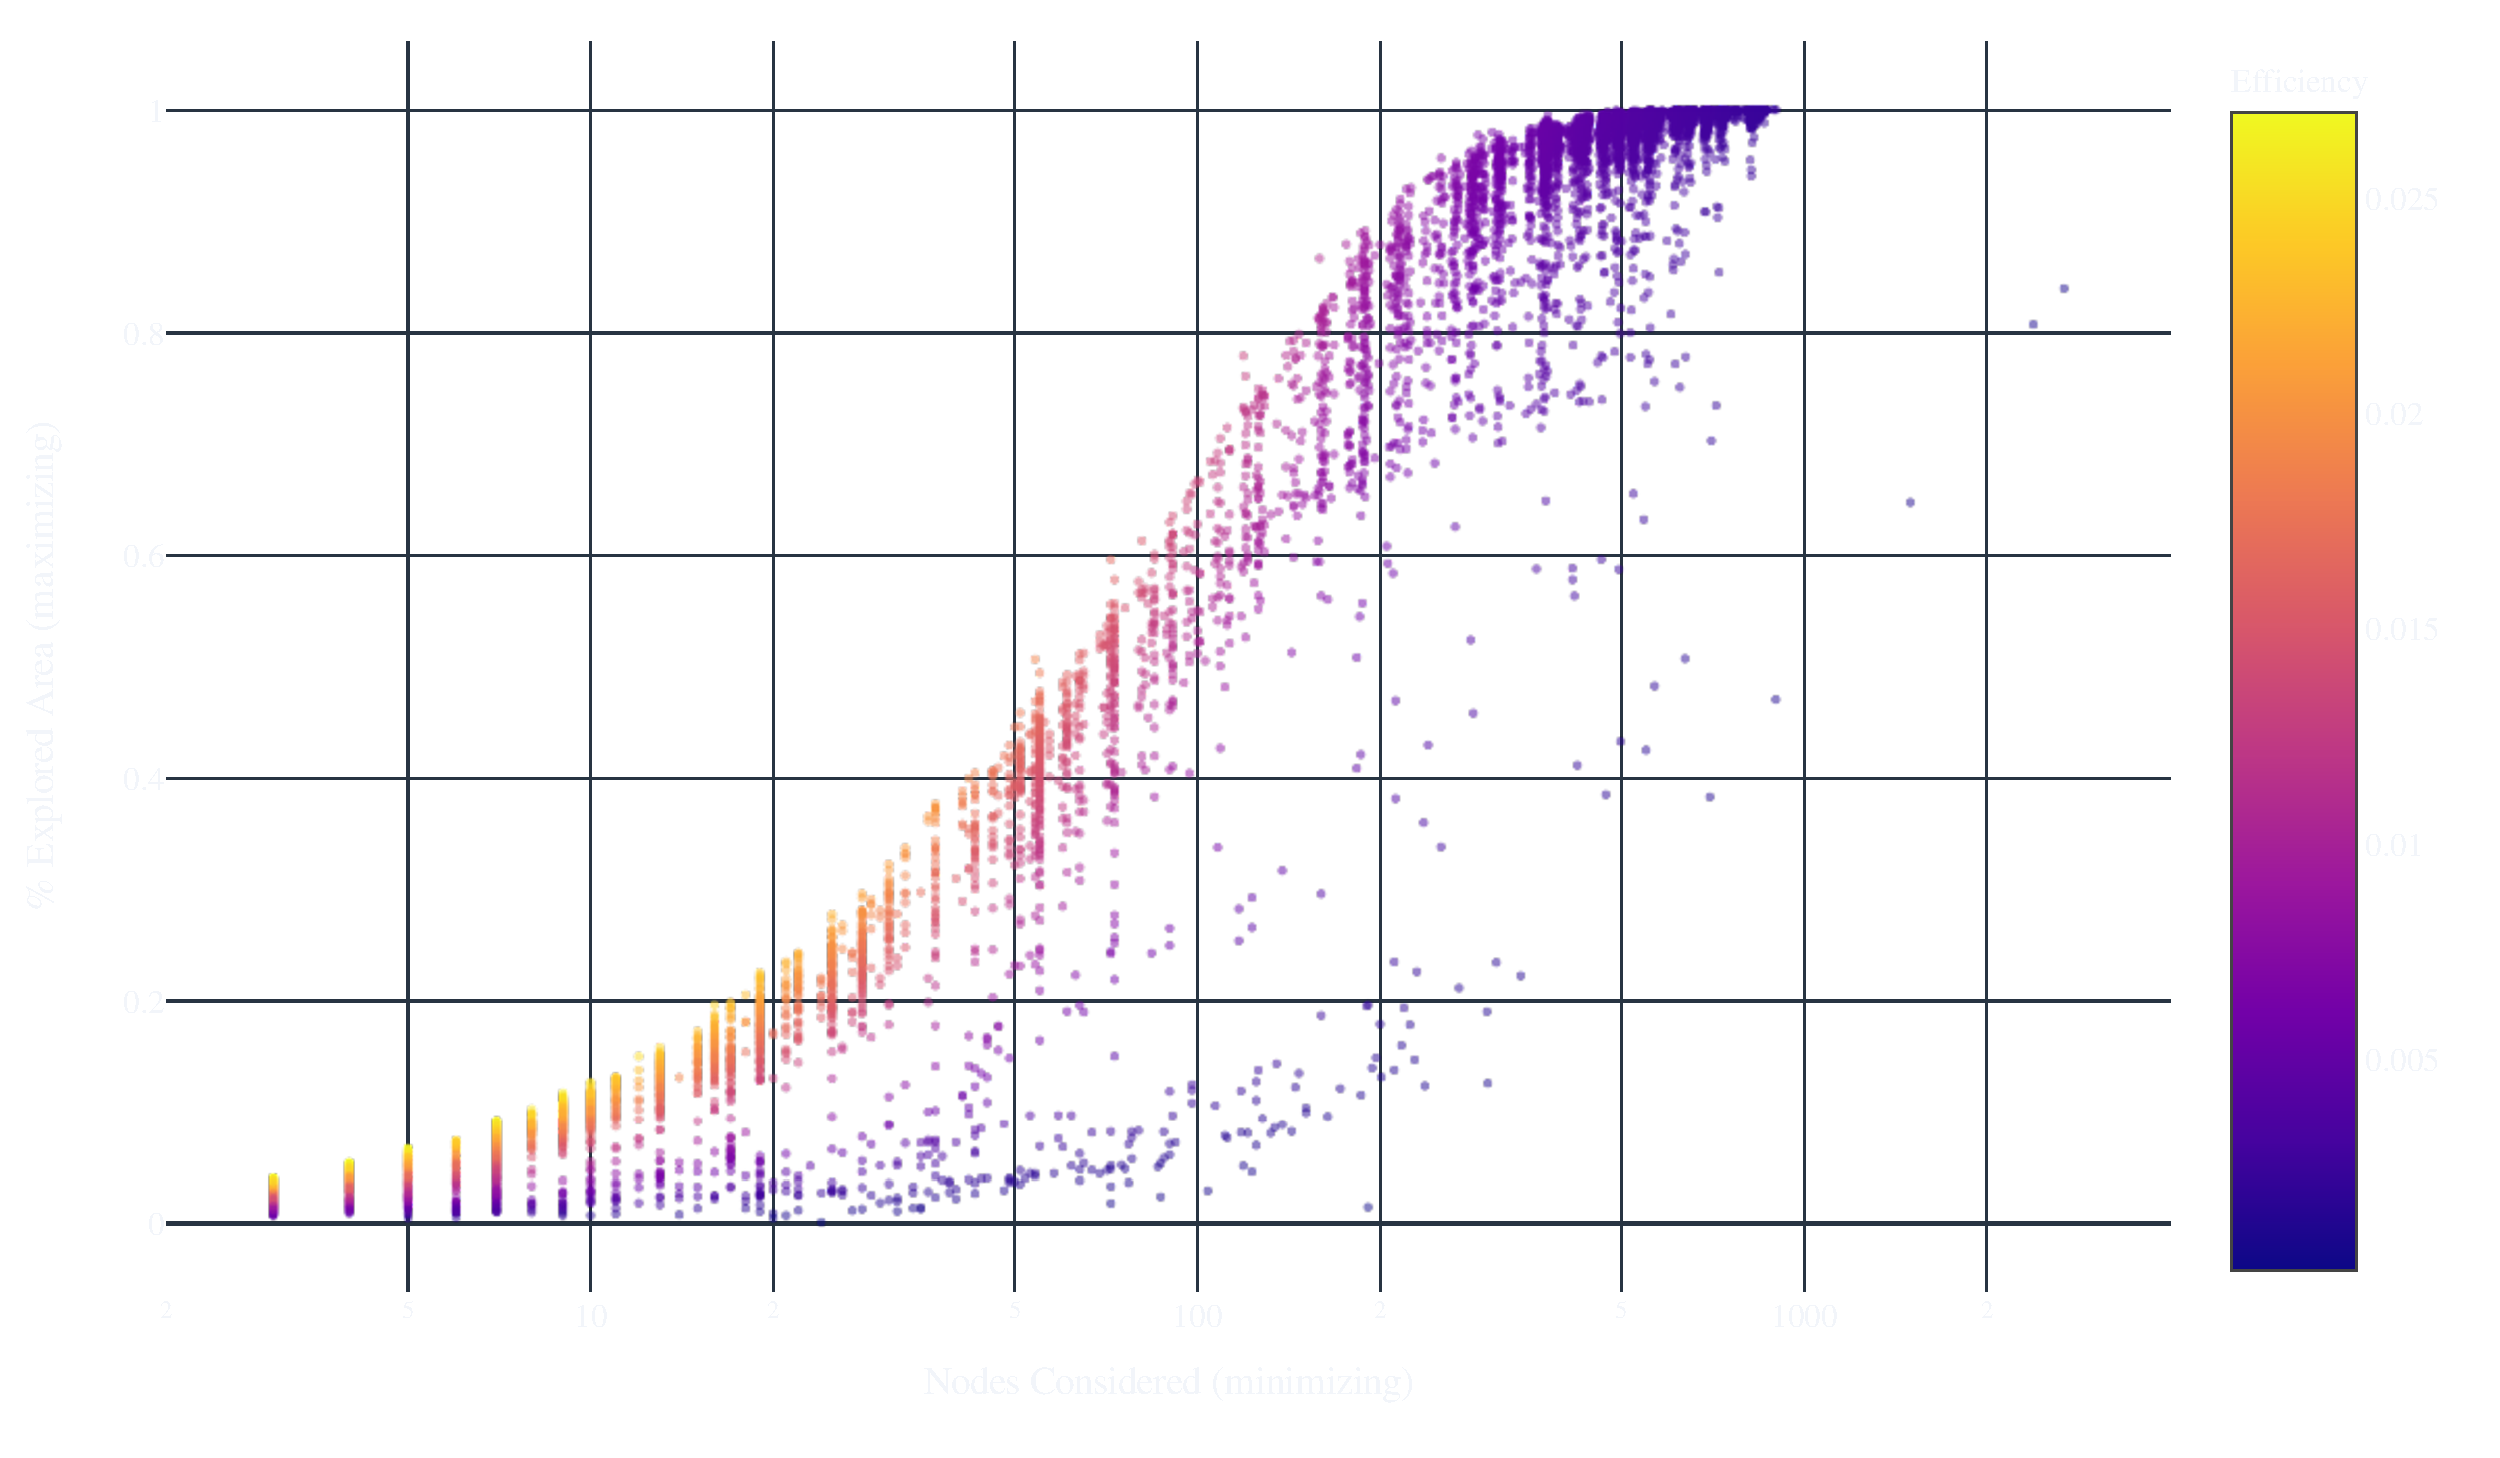
\includegraphics[width=0.85\linewidth, keepaspectratio]{figures/efficient_overview.pdf}
\end{frame}

\begin{frame}{Challenges Faced}
    \begin{vfilleditems}
    \item \Huge Test
    \end{vfilleditems}
\end{frame}

\begin{frame}{\white{Experiment Types}}
    \begin{vfilleditems}
    \item \emph{Improve}
    \item \emph{Select}
    \item \emph{Fix}
    \end{vfilleditems}
\end{frame}

\begin{frame}{Gritty Engineering Work}
    \begin{vfilleditems}
    \item \Huge Test
    \end{vfilleditems}
\end{frame}

\begin{frame}{Future Work}
    \begin{vfilleditems}
    \item \Huge Test
    \end{vfilleditems}
\end{frame}

\begin{frame}{Strong Ending}
    \centering
    \vfill
    {\fontsize{40}{50}\selectfont Final Figure and Remarks}
    \vfill
\end{frame}

\begin{frame}[plain]{}
  \begin{figure}
  \centering
  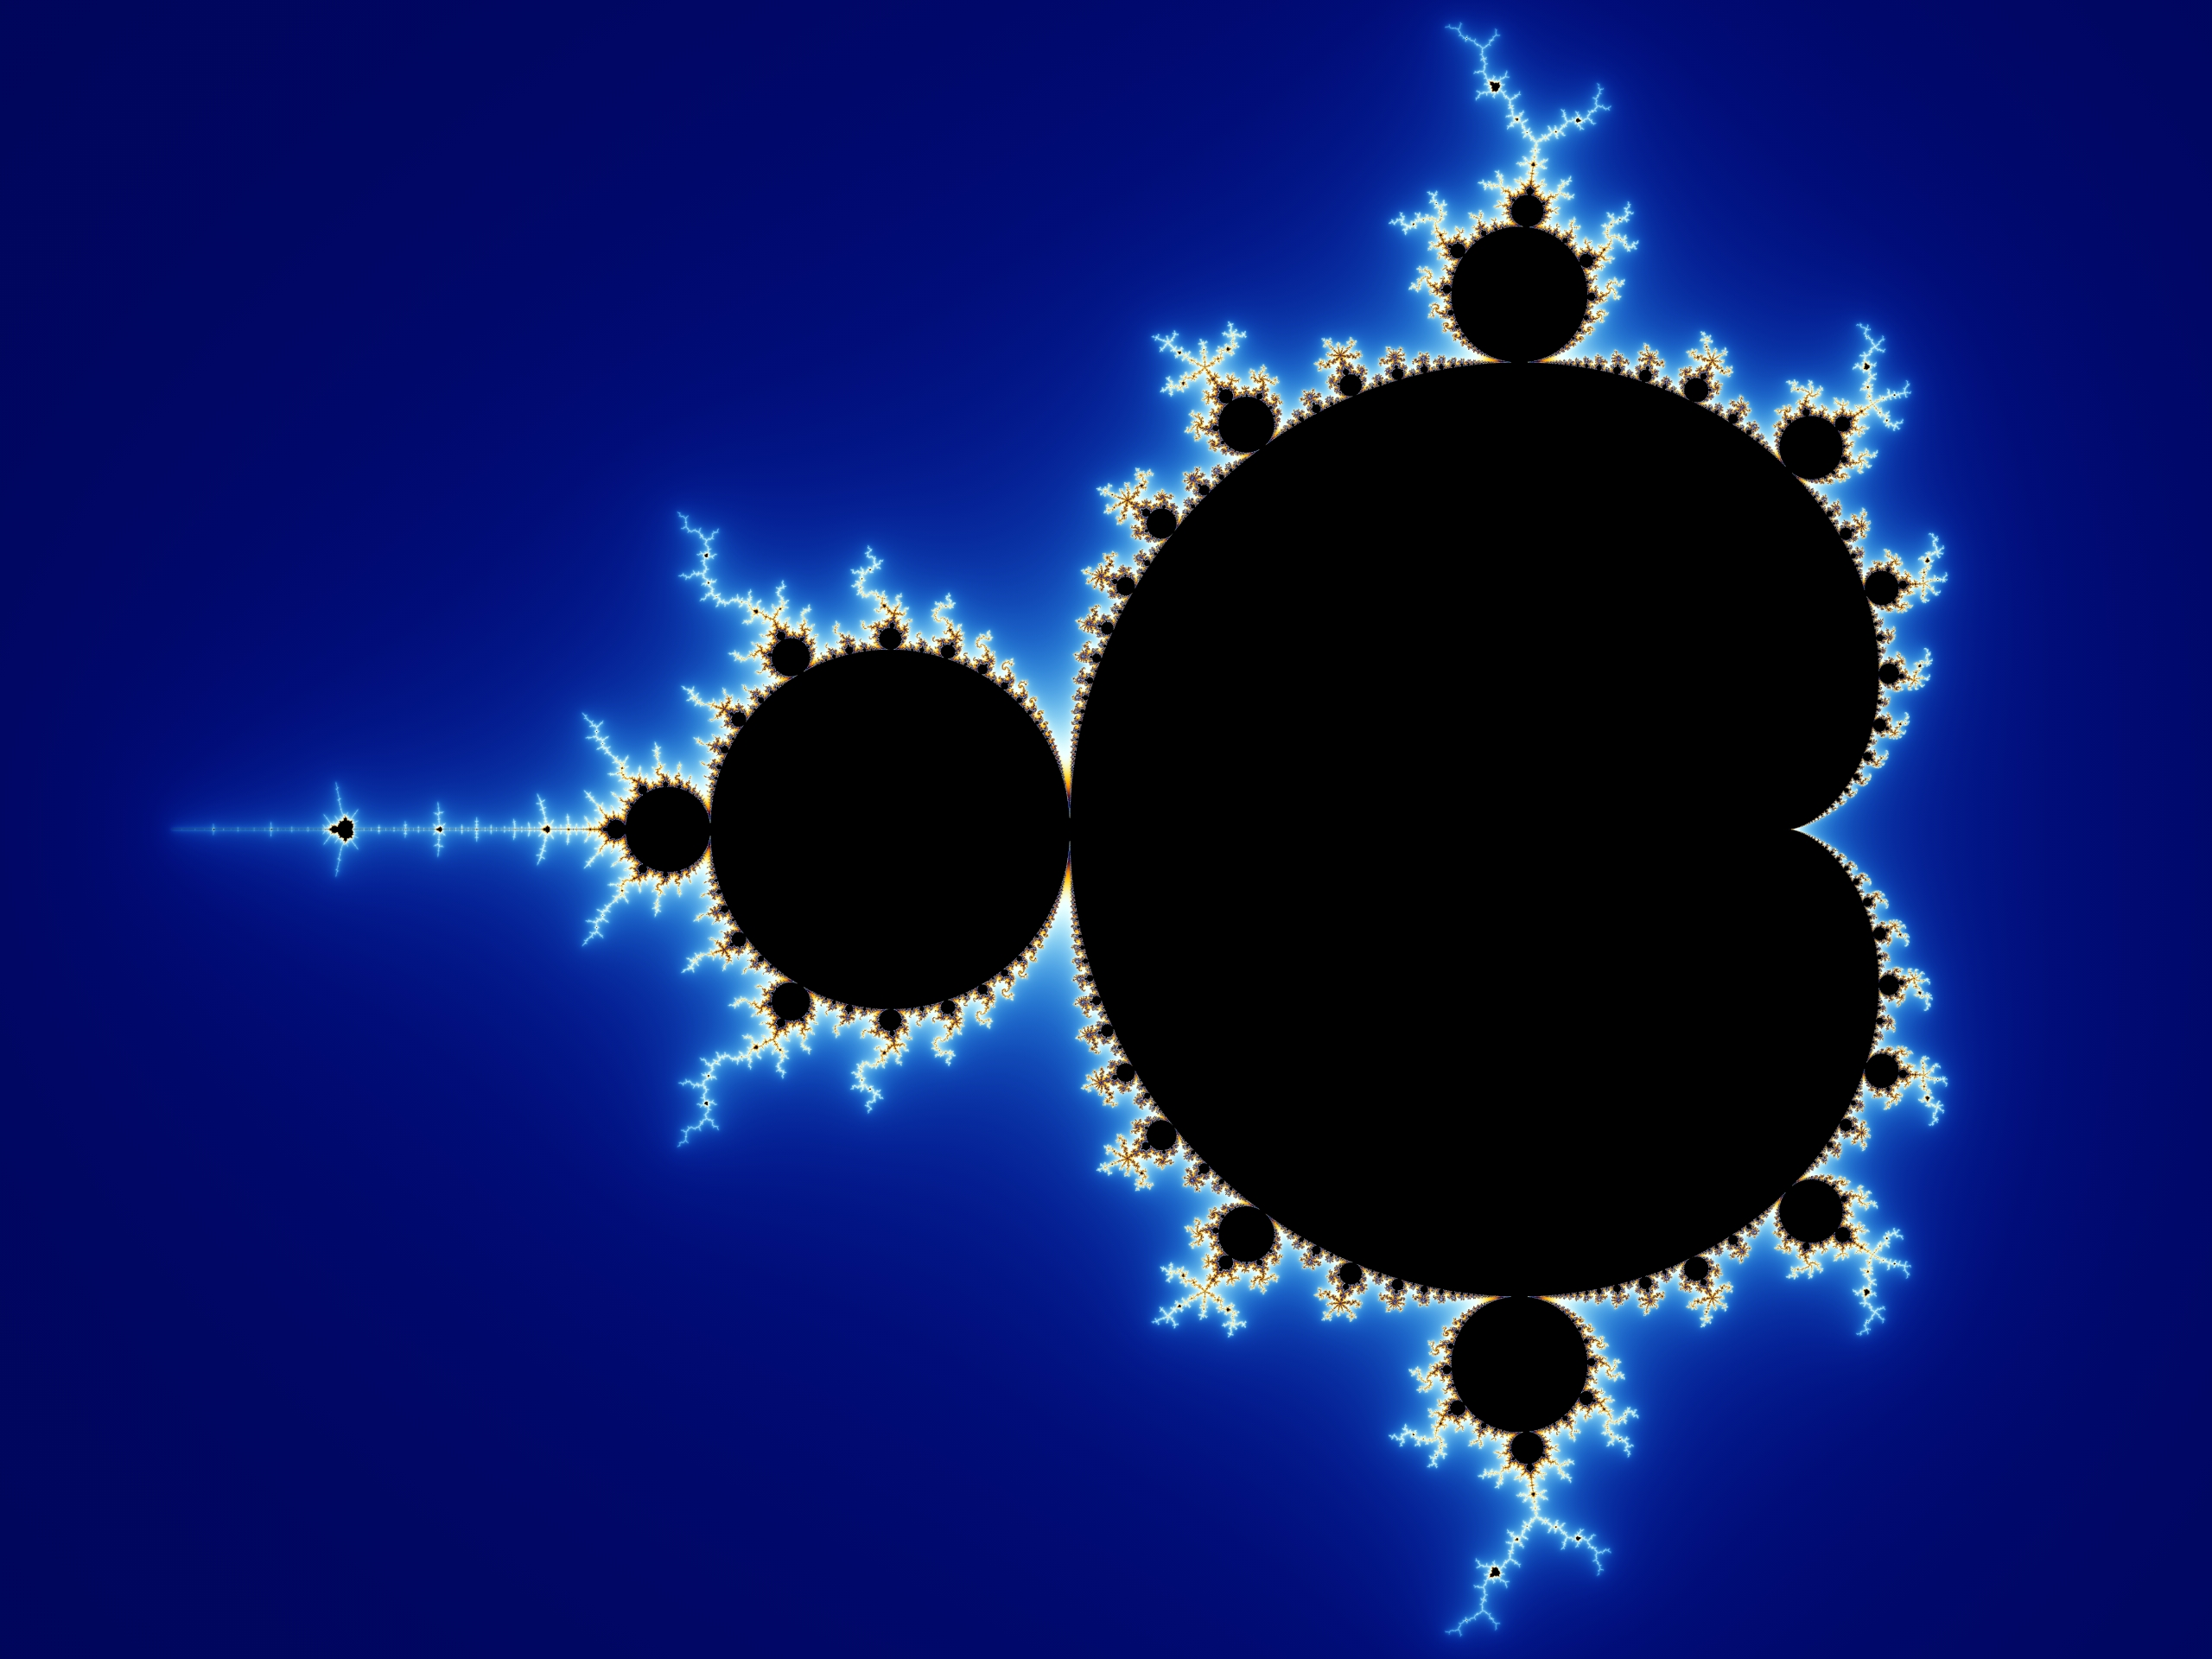
\includegraphics[height=1.0\textheight,keepaspectratio]{figures/mandelbrot.jpg}
  \end{figure}
\end{frame}

\begin{frame}[plain]{}
  \begin{figure}
  \centering
  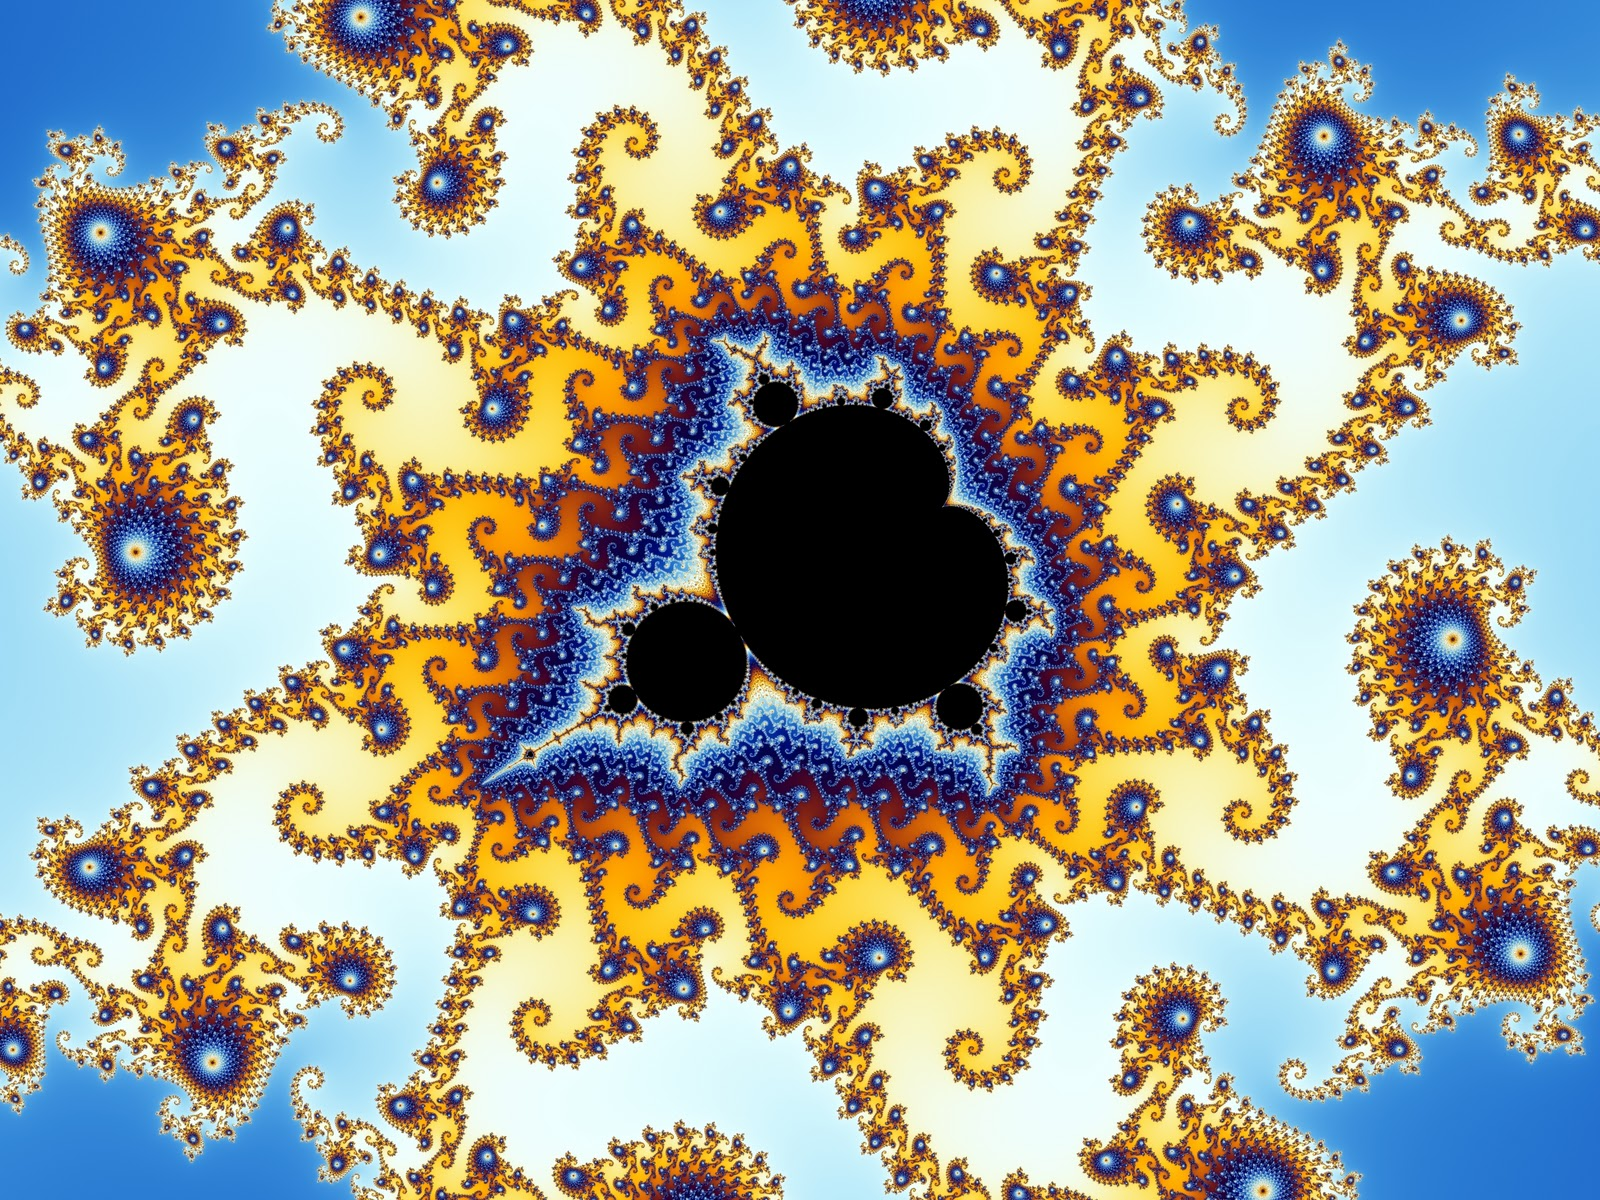
\includegraphics[width=1.0\linewidth,keepaspectratio]{figures/mandelbrot_2.jpg}
  \end{figure}
\end{frame}

\begin{frame}{Program Synthesis}
\begin{vfilleditems}
    \item \Huge Kolmogorov
    \item \Huge Schmidhuber
    \item \Huge Lenat
    \item \emph{Lenat}
\end{vfilleditems}
\end{frame}

\appendix % do not count the following slides for the total number
\section*{Backup Slides}

\begin{frame}[plain, noframenumbering]
  \centering
  \vfill
  {\fontsize{40}{50}\selectfont Questions?}
  \vfill
\end{frame}


\begin{frame}[plain, noframenumbering]
  \centering
  \printbibliography
\end{frame}

\begin{frame}{Population Dynamics: Baldur's Gate}
    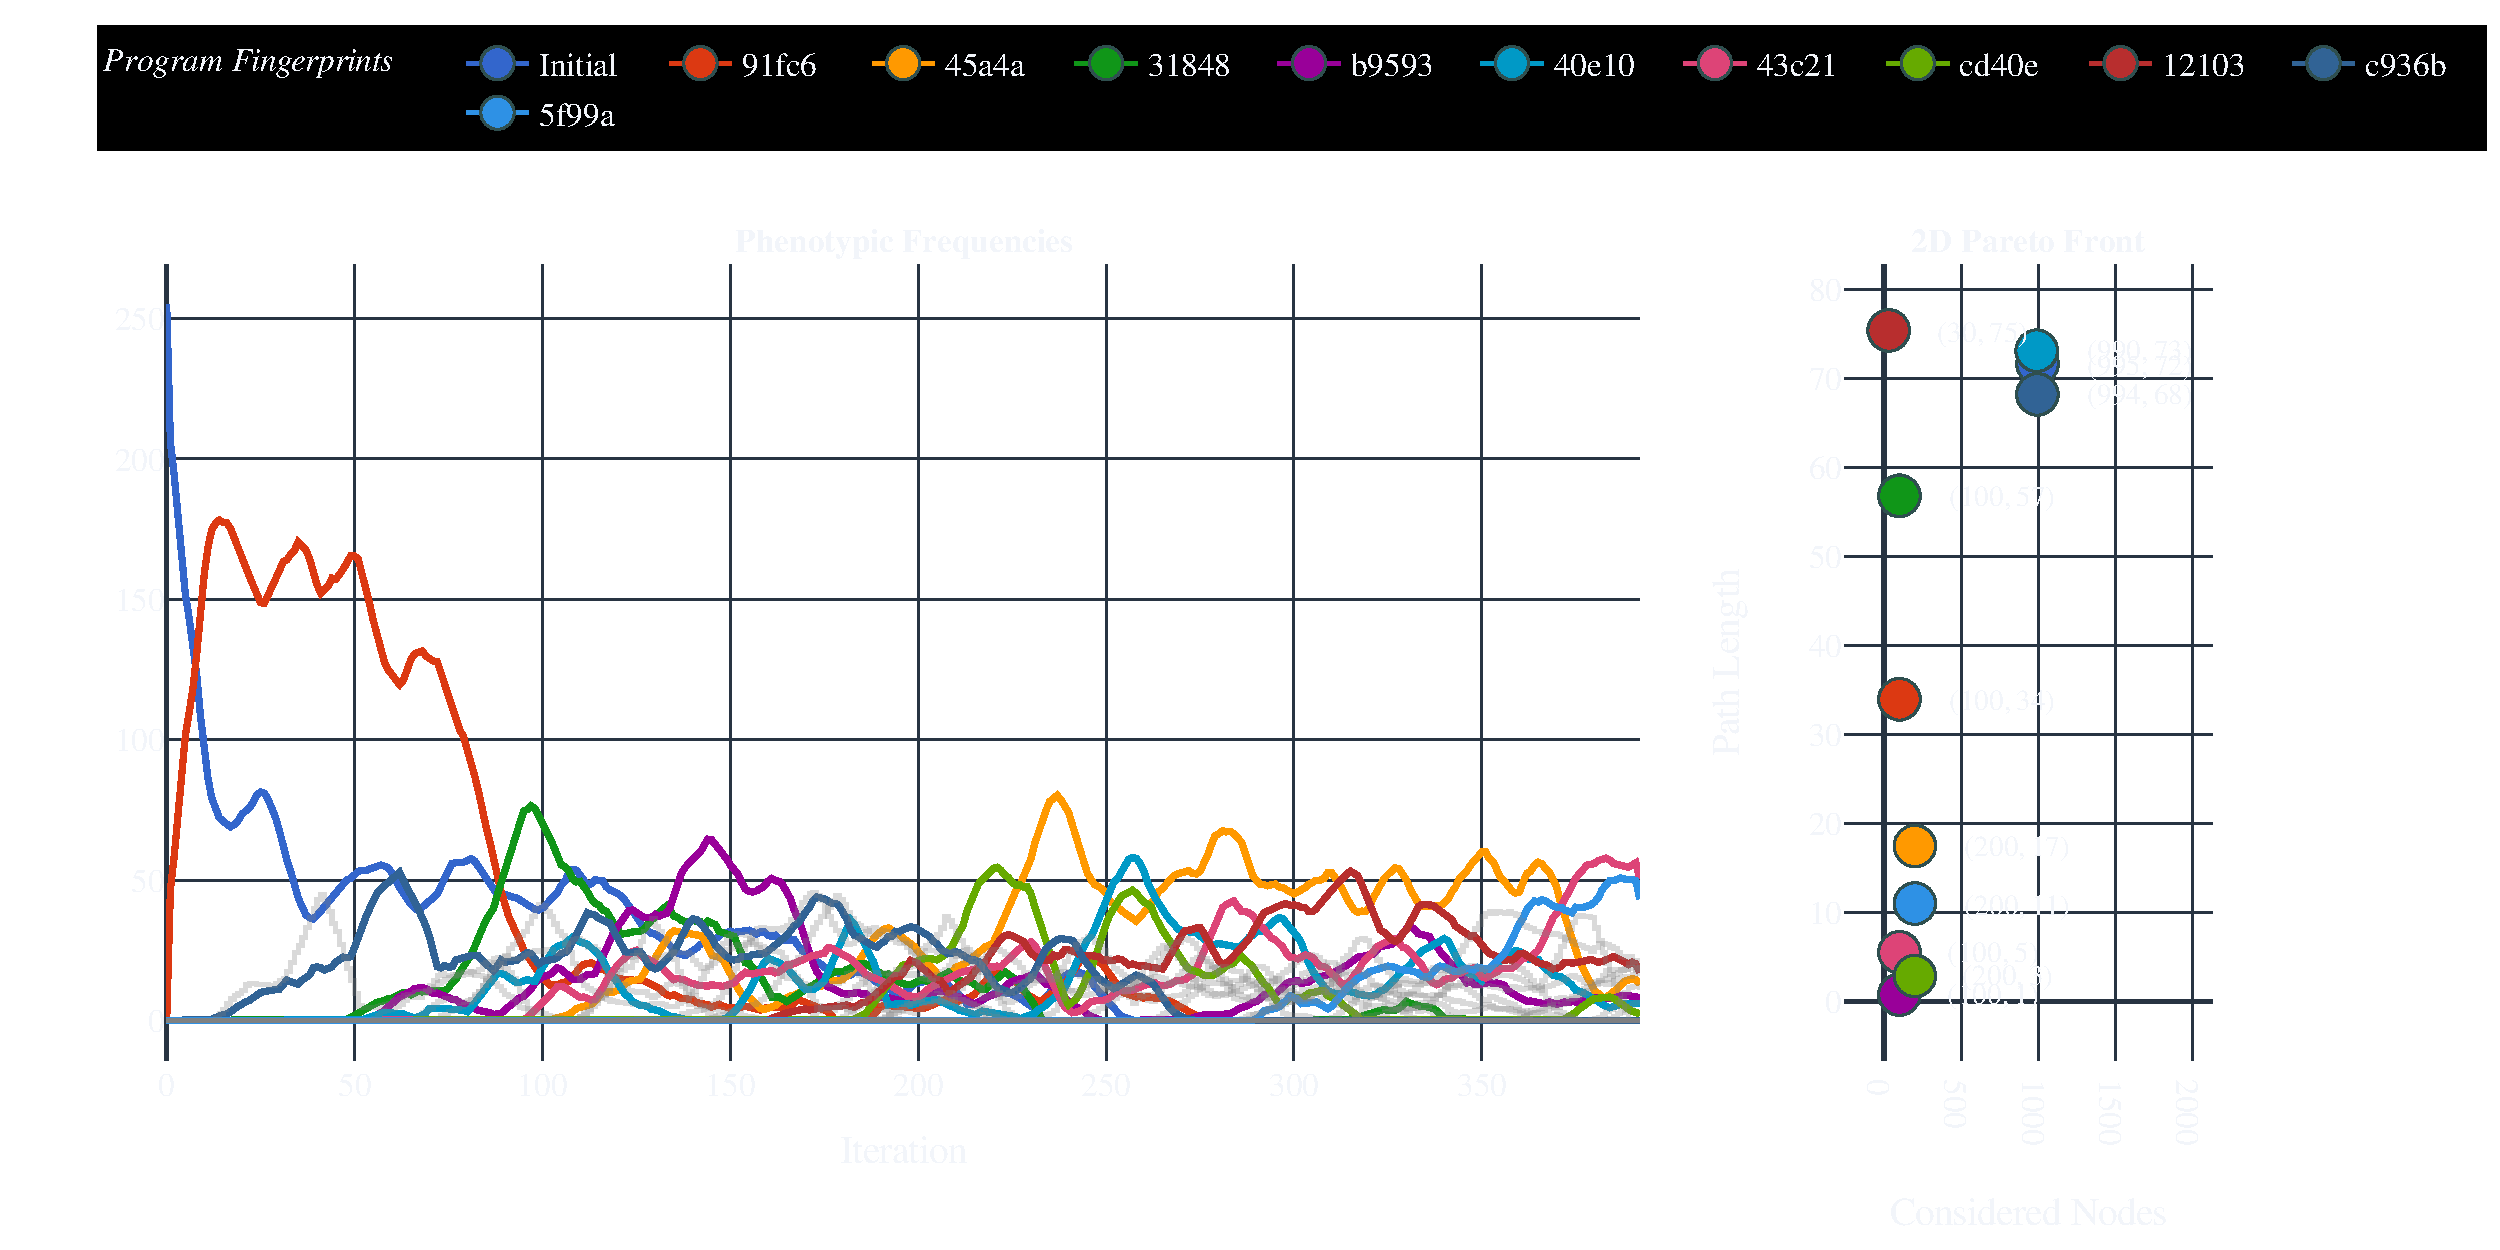
\includegraphics[width=1.0\linewidth, keepaspectratio]{figures/baldurs_pheno_50.pdf}
\end{frame}

\begin{frame}{Milan overview}
    \centering
    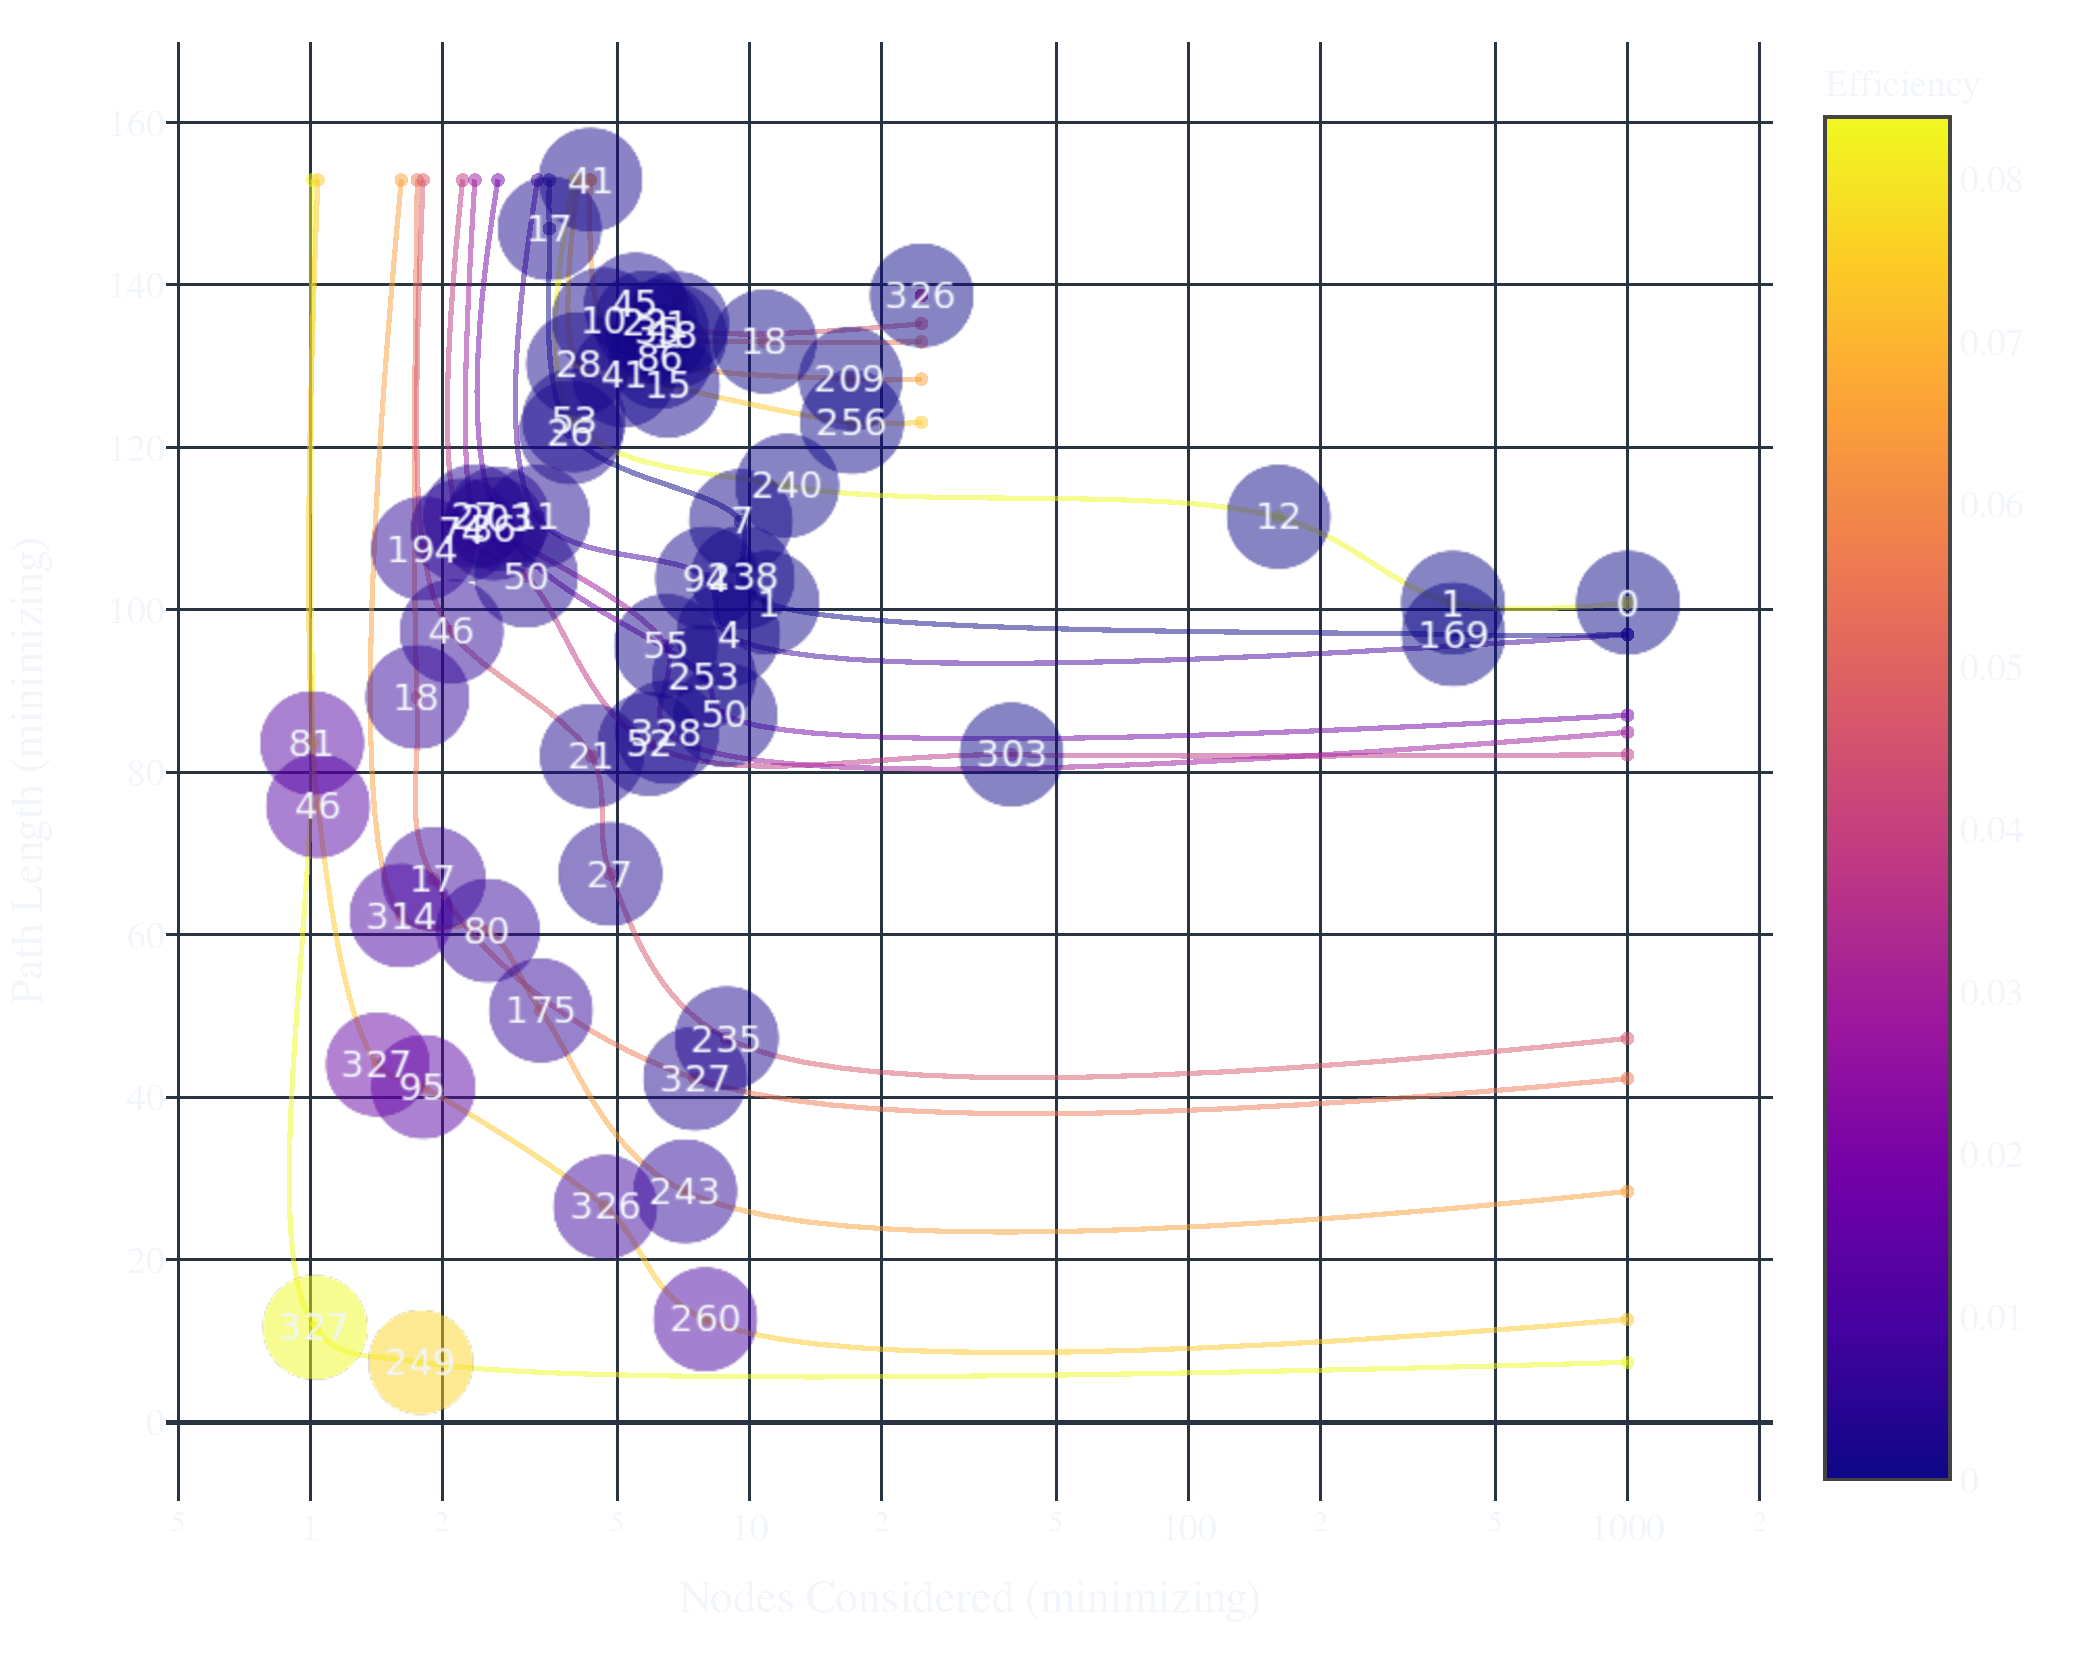
\includegraphics[width=0.5\linewidth, keepaspectratio]{figures/milan_total_pareto_overview.pdf}
\end{frame}

\begin{frame}[plain, noframenumbering]{Test}
\begin{overpic}[width=1.0\textwidth,grid,tics=10]{figures/perseverance.jpg}
 \put (20,85) {\color{black}\huge$\displaystyle\gamma$}
\end{overpic}
\end{frame}

\begin{frame}[plain]{Thesis}
    \begin{vfilleditems}
      \item {\Huge Evolution is powerful}
        \begin{itemize}
          \item {\Medium Responsible for Earth's diverse, adaptive life}
          \item {\Medium \color{pureminimalistic@text@red} Evolved intelligence}
        \end{itemize}
      \item {\Huge Learned representation matters}
    \end{vfilleditems}
\end{frame}

\begin{frame}{Research Questions}
  \begin{vfilleditems}
    \item {\Huge Is Genetic Programming Competitive in 2021? {\color{pureminimalistic@text@red} Yes.}}
    % TODO: Answer each at high level
    {\color{grey}
    \item {\Huge Is crossover necessary?}
    \item {\Huge What is the role of latent code?}
    \item {\Huge How should code be mutated?}
    \item {\Huge How hard is a problem?}
    }
  \end{vfilleditems}
\end{frame}

\begin{frame}{Research Questions}
  \begin{vfilleditems}
    \item {\Huge Role of program representation?}
    \item {\Huge Role of scale and compute efficiency?}
    \item {\Huge How should code be mutated?}
    \item {\Huge How hard is a problem?}
  \end{vfilleditems}
\end{frame}


\end{document}